% !TEX root = main.tex
\documentclass[11pt,a4paper,spanish, oneside]{book}
\usepackage{array}
\usepackage{estilo_unir-1}
\usepackage{apacite}

\usepackage{hyperref}
\numberwithin{equation}{chapter}
%\usepackage{caption}
\numberwithin{figure}{chapter}
\usepackage{longtable, booktabs, ragged2e, multirow, tabularx}
%\usepackage{chngcntr}
%\counterwithin{equation}{chapter}
%\counterwithin{figure}{chapter}
%\counterwithin{table}{chapter}
%\renewcommand\theequation{\thechapter.\arabic{equation}}
%\renewcommand\thefigure{\thechapter.\arabic{figure}}
%\renewcommand\thetable{\thechapter.\arabic{table}}
%\renewcommand\theequation{\thechapter.\arabic{equation}}
%\counterwithin{figure}{chapter}
%\counterwithin{table}{chapter}
%\renewcommand\thefigure{\thechapter.\arabic{figure}}
%\renewcommand\thetable{\thechapter.\arabic{table}}
%\renewcommand\thefigure{\thechapter.\arabic{figure}}
%\makeatletter
%\renewcommand\p@figure{\thechapter..\arabic{figure}}
%\makeatother



%---------------------------
%titulo del trabajo y autor
%---------------------------
\title{Sistema inteligente de apoyo a la decisión para puestos de mando de emergencias}
\titulacion{Máster Universitario en Inteligencia Artificial}
\author{Juan Carlos Albert Fillol, Ancor González Carballo y Brian Mathias Pesci Juliani}
\date{24 de junio de 2026}
\director{Dr. Andrés Soto Villaverde}
\nombreciudad{Madrid, Tenerife y Alicante}

%---------------------------
%marges
%---------------------------
%\usepackage[margin=1.9cm]{geometry}
%---------------------------
%---------------------------
%---------------------------
%---------------------------
\begin{document}
\renewcommand{\listfigurename}{Indice de Ilustraciones}
\renewcommand{\listtablename}{Indice de Tablas}
\renewcommand{\contentsname}{Indice de Contenidos}
\renewcommand{\figurename}{Figura}
\renewcommand{\tablename}{Tabla} 

% Portada inlined para que pandoc/docx procese el logo
\makeatletter
\begingroup
\thispagestyle{empty}

\includegraphics[width=0.8\textwidth]{figures/logo_unir}

\vspace{1cm}
\centering{
\begin{tabular}{!{\color{azulunir}\vrule width 2pt}p{12cm}}
{\Large {\bf Universidad Internacional de la Rioja (UNIR)}} \\ \vspace{0.1cm}
{ \huge {\bf Escuela Superior de Ingeniería y Tecnología}} \\ \vspace{0.1cm}
{ \Large {\bf \@titulacion}}\\ \vspace{1cm}
{\Huge {\bf {\color{azulunir}{\thetitle} }  }  }
\end{tabular}
}
\vfill

\noindent
\flushleft{
{\bf Trabajo Fin de Estudios}\\  \vspace{0.3cm}
{\bf Presentado por:} \theauthor\\  \vspace{0.3cm}
{\bf Dirigido por:} \@director
}
\vspace{3cm}

{\color{azulunir}{Ciudad:}}\@nombreciudad\\
{\color{azulunir}{Fecha:}} \thedate
\newpage
\thispagestyle{empty}
\endgroup
\makeatother

\frontmatter
\tableofcontents
\listoffigures
\listoftables

\chapter*{Resumen}
\addcontentsline{toc}{chapter}{Resumen}

La gestión de emergencias civiles exige decisiones rápidas y fundamentadas bajo entornos de alta presión temporal e incertidumbre. Este trabajo diseña, implementa y evalúa un prototipo neuro-simbólico modular de apoyo a la decisión para la priorización explicable de incidentes 112 en Castilla y León. El sistema utiliza el Registro de Emergencias (2008--2022) para definir una escala académica de prioridad P1--P4 mediante supervisión débil. La arquitectura consta de tres capas: Capa 1 (procesamiento de lenguaje natural en español e ingesta experimental de llamadas de voz mediante ASR local con Whisper), Capa 2 (núcleo decisor interpretable con RuleFit-lite respaldado por salvaguardas deterministas) y Capa 3 (generación de explicaciones normativas mediante LLM local, RAG y Model Context Protocol). Evaluamos cuantitativamente la propuesta frente a un baseline experto de 19 reglas y una variante diagnóstica con \texttt{imodels} usando validación estratificada y temporal, control anti-\textit{leakage} y análisis de sesgos. Además, se analizan la fidelidad de las explicaciones y la usabilidad percibida mediante un estudio piloto con 9 participantes. Los resultados confirman que RuleFit-lite alcanza una macro-F1 de 0,905 y una sensibilidad P1 del 0,910, mejorando significativamente a la línea base y manteniendo la latencia y trazabilidad requeridas en salas de control. El prototipo se valida como una base académica reproducible para el diseño de sistemas interactivos (Human-in-the-loop) alineados con la normativa de IA europea.

\medskip
\textbf{Palabras clave:} emergencias 112, sistemas de apoyo a la decisión (DSS), inteligencia artificial explicable (XAI), arquitectura neuro-simbólica, supervisión débil, RuleFit, reconocimiento del habla (ASR).

\chapter*{Abstract}
\addcontentsline{toc}{chapter}{Abstract}

Civil emergency management requires rapid, evidence-based decisions under high time pressure and uncertainty. This thesis designs, implements, and evaluates a modular neuro-symbolic decision-support prototype for explainable 112 incident prioritization in Castilla y Leon. The system leverages the 2008--2022 Emergency Registry to build an academic P1--P4 priority scale using weak supervision. The architecture is organized in three layers: Layer 1 (Spanish NLP processing and experimental voice call ingestion via local ASR with Whisper), Layer 2 (interpretable decision core using RuleFit-lite backed by deterministic safeguards), and Layer 3 (normative explanation generation through a local LLM, RAG, and Model Context Protocol). The proposal is quantitatively evaluated against a 19-rule expert baseline and a diagnostic \texttt{imodels} variant using stratified and temporal splits, anti-leakage controls, and bias checks. In addition, explanation fidelity and perceived usability are assessed via a pilot study with 9 participants. Results show that RuleFit-lite achieves a macro-F1 of 0.905 and a P1 recall of 0.910, significantly outperforming the baseline while preserving the latency and traceability required in control rooms. The prototype validates a reproducible academic basis for human-in-the-loop systems aligned with European AI regulations.

\medskip
\textbf{Keywords:} 112 emergencies, decision support systems (DSS), explainable artificial intelligence (XAI), neuro-symbolic architecture, weak supervision, RuleFit, automatic speech recognition (ASR).




\mainmatter
\chapter*{Organización del trabajo en grupo}
\addcontentsline{toc}{chapter}{Organización del trabajo en grupo}
\setcounter{secnumdepth}{-1}

\section{Introducción al trabajo grupal}

El presente Trabajo Fin de Máster (TFM) se ha desarrollado en modalidad grupal, de conformidad con el procedimiento establecido por la Universidad Internacional de La Rioja (UNIR). Esta modalidad resulta coherente con la naturaleza del proyecto: se diseña, implementa y evalúa un sistema inteligente de apoyo a la decisión para la priorización temprana de incidentes 112 en Castilla y León, combinando procesamiento del lenguaje natural, aprendizaje interpretable, explicación normativa y desarrollo de software.

La organización del equipo se articula en tres capas funcionales y una función transversal de integración. La Capa 1 estructura el texto operativo en variables y señales predecisionales. La Capa 2, desarrollada como bloque metodológico central, transforma esas señales en una recomendación P1--P4 interpretable y evaluable. La Capa 3 convierte la recomendación en una explicación operativa mediante un modelo de lenguaje de gran tamaño (\textit{Large Language Model}, LLM) local, generación aumentada por recuperación (\textit{Retrieval-Augmented Generation}, RAG) y herramientas basadas en \textit{Model Context Protocol} (MCP).

El reparto no se limita a distribuir tareas de programación. Cada integrante asume una contribución diferenciada al componente inteligente del sistema, de modo que el resultado conjunto pueda defenderse como una solución integrada y no como una suma de piezas independientes.

\section{Integrantes del equipo y roles asignados}

El equipo está formado por tres estudiantes del Máster Universitario en Inteligencia Artificial de la UNIR, bajo la dirección del Dr. Andrés Soto Villaverde. Cada integrante aporta un perfil complementario y una responsabilidad principal dentro de la arquitectura.

\subsection{Capa 1: extracción de variables operativas}
\textbf{Responsable principal:} Ancor González Carballo.

Su bloque de trabajo se orienta a la transformación del texto libre del incidente en una representación estructurada compatible con la priorización posterior. Esta capa combina procesamiento del lenguaje natural auditable, detección de señales operativas, tratamiento de negaciones y normalización de variables V01--V15. En la versión evaluada se presenta como un extractor determinista y reproducible; la incorporación de clasificadores aprendidos queda como evolución futura sujeta a una validación específica. Esta contribución es importante porque la calidad de la priorización depende de que el sistema represente correctamente el incidente antes de aplicar reglas o modelos.

\subsection{Capa 2: supervisión débil, RuleFit y evaluación}
\textbf{Responsable principal:} Juan Carlos Albert Fillol.

Su bloque de trabajo se centra en convertir datos reales e incompletos del Registro 112 Castilla y León en una recomendación de prioridad interpretable, evaluable y trazable. Para ello formaliza la escala académica P1--P4, audita el conjunto de datos, construye etiquetas mediante supervisión débil, define una línea base heurística, selecciona RuleFit-lite como motor interpretable y evalúa el comportamiento del sistema mediante macro-F1, sensibilidad de P1, estabilidad temporal, análisis por subgrupos y errores críticos.

Juan Carlos asume, además, la coordinación metodológica y el cierre del bloque de datos, supervisión débil, línea base heurística, priorización interpretable, evaluación, revisión interna y trazabilidad de Capa 2. Su aportación conecta la salida de Capa 1 con la explicación de Capa 3, sin asumir la autoría de las capas desarrolladas por los demás integrantes.

\subsection{Capa 3: explicación generativa y recuperación normativa}
\textbf{Responsable principal:} Brian Mathias Pesci Juliani.

Su bloque de trabajo comprende la explicación y la integración conceptual del prototipo. Incluye la recuperación normativa, la explicación generativa local y la trazabilidad de la inferencia. Su contribución consiste en convertir la salida del modelo interpretable en una recomendación comprensible y revisable, sin modificar la prioridad calculada por Capa 2 y manteniendo la ejecución local de los datos sensibles.

\section{Distribución de capítulos y anexos}

La Tabla~\ref{tab:tab1secCTF} recoge la distribución de responsabilidades sobre la memoria. El reparto final se ha definido con un único responsable por archivo para evitar duplicidades, solapamientos y conflictos de integración. De esta forma, cada integrante revisa su parte, identifica los cambios necesarios y aporta texto, evidencias, capturas o referencias para la unificación final.

\begin{table}[htbp]
\centering
\scriptsize
\setlength{\tabcolsep}{4pt}
\begin{tabular}{|p{4.2cm}|p{4.2cm}|p{4.6cm}|}
\hline
\textbf{Apartado / capítulo} & \textbf{Responsables} & \textbf{Tipo de contribución} \\ \hline
\texttt{chap0.tex} & Juan Carlos & Organización del trabajo y reparto final \\ \hline
\texttt{chap1.tex} & Juan Carlos & Introducción, problema, alcance y contribución IA \\ \hline
\texttt{chap2.tex} & Brian & Contexto, estado del arte y bibliografía APA 7 \\ \hline
\texttt{chap3.tex} & Ancor & Marco operativo, normativo y contexto 112 CyL \\ \hline
\texttt{chap4.tex} & Juan Carlos & Objetivos, preguntas de investigación y metodología \\ \hline
\texttt{chap5.tex} & Ancor & Requisitos y especificación funcional \\ \hline
\texttt{chap6.tex} & Brian & Arquitectura, contratos y diseño del sistema \\ \hline
\texttt{chap7.tex} & Juan Carlos & Datos de Castilla y León, supervisión débil, prevención de fugas y particiones \\ \hline
\texttt{chap8.tex} & Brian & Integración del prototipo y demostración funcional \\ \hline
\texttt{chap9.tex} & Juan Carlos & Evaluación de Capa 2, integración, revisión preparada y análisis por subgrupos \\ \hline
\texttt{chap10.tex} & Ancor & Conclusiones, limitaciones y trabajo futuro \\ \hline
\texttt{anexo\_a.tex}, \texttt{anexo\_b.tex}, \texttt{anexo\_g.tex} & Ancor & Taxonomía, variables y guía de uso \\ \hline
\texttt{anexo\_c.tex}, \texttt{anexo\_d.tex}, \texttt{anexo\_e.tex} & Juan Carlos & Guía P1--P4, protocolo de revisión y línea base heurística \\ \hline
\texttt{anexo\_f.tex}, \texttt{anexo\_h.tex}, \texttt{anexo\_l.tex}; \texttt{bibliografia.bib} & Brian & Correspondencia conceptual-software, transparencia, corpus normativo consolidado, fichas de modelo y bibliografía \\ \hline
\end{tabular}
\caption{Distribución de capítulos, responsables y tipo de contribución.}
\label{tab:tab1secCTF}
\smallskip
{\small\textit{Fuente: elaboración propia.}\par}
\end{table}

\section{Metodología de coordinación del grupo}

La coordinación se ha apoyado en reuniones periódicas, control de versiones y una planificación por tareas trazables. Las decisiones de alcance se documentan de forma común y los contratos de datos permiten que cada capa avance sin romper la integración.

El equipo ha trabajado con una lógica iterativa e incremental. Primero se fijaron los acuerdos de integración y la constitución del proyecto; después se definieron el conjunto de datos, la guía de etiquetado y el corpus normativo; posteriormente se implementaron las capas técnica y explicativa; y finalmente se orienta el trabajo hacia la evaluación, la redacción y la defensa. Esta organización permite mantener alineados el prototipo software, la memoria académica y la evidencia reproducible.

De este modo, la organización del trabajo refleja la idea central del TFM: diseñar, implementar y evaluar un sistema de apoyo a la decisión para incidentes 112 en Castilla y León, con prioridad explicable P1--P4, supervisión humana, soberanía del dato y trazabilidad normativa.

\setcounter{secnumdepth}{2}

\chapter{Introducción}
\label{cap:1}

\section{Contexto general del trabajo}

La gestión de emergencias es uno de los ámbitos de actuación pública donde la rapidez y la calidad de las decisiones tienen consecuencias más directas sobre la vida de las personas. En los primeros minutos de un incidente, el operador del 112 o el responsable de coordinación debe interpretar información incompleta, heterogénea y a menudo cambiante: texto libre de la llamada, categoría preliminar, localización, número de afectados, señales de riesgo, condiciones territoriales y posible necesidad de escalar la respuesta.

El marco español de protección civil, articulado principalmente por la Ley 17/2015 y la Norma Básica de Protección Civil, establece una respuesta basada en coordinación, planificación y actuación graduada ante diferentes riesgos \cite{Ley17_2015,RD524_2023}. En Castilla y León, este marco se concreta mediante la Ley 4/2007, el Plan Territorial de Protección Civil de Castilla y León (PLANCAL) y diversos planes especiales como INFOCAL, INUNCYL o MPCyL \cite{Ley4_2007_CYL,PLANCAL_DEC_4_2019,INFOCAL_DEC_6_2025,INUNCYL,MPCYL_ACUERDO_3_2008}. Este entorno normativo proporciona una base adecuada para construir un sistema de apoyo a la decisión que no se limite a clasificar incidentes, sino que justifique sus recomendaciones con criterios operativos y trazabilidad documental.

El presente TFM se sitúa en la intersección entre gestión de emergencias e inteligencia artificial aplicada. Su objetivo es diseñar, implementar y evaluar un prototipo software modular que priorice incidentes 112 de Castilla y León en una escala académica P1--P4, ofreciendo al operador una recomendación explicable, revisable y respaldada por reglas, evidencias internas y trazabilidad documental. La escala P1--P4 utilizada en el trabajo no corresponde a una prioridad oficial del servicio 112, sino a una construcción académica necesaria para entrenar, evaluar y explicar el prototipo. El sistema no sustituye al operador humano ni moviliza recursos de forma autónoma: actúa como herramienta de apoyo a la primera decisión.

\section{Planteamiento del problema}

La saturación informativa en emergencias aparece cuando el volumen, la velocidad o la heterogeneidad de la información supera la capacidad del operador para procesarla con seguridad. Este fenómeno es crítico en situaciones con múltiples incidentes simultáneos, avisos incompletos o información contradictoria. En esos escenarios, una priorización deficiente puede retrasar la atención a incidentes graves, sobredimensionar sucesos menores o dificultar la justificación posterior de la decisión adoptada.

El problema abordado por este TFM puede formularse así: dado un conjunto de incidentes 112 descritos mediante texto libre y datos operativos parciales, ¿cómo puede un sistema inteligente ayudar a estructurar la información, extraer variables relevantes, recomendar una prioridad P1--P4 y explicar esa recomendación de forma comprensible y auditable?

La respuesta propuesta se apoya en una arquitectura de tres capas. La Capa 1 transforma texto operativo en variables y señales predecisionales mediante procesamiento del lenguaje natural auditable, detección de negaciones y normalización operativa. La Capa 2 recomienda la prioridad mediante RuleFit-lite y se compara con una línea base heurística y una implementación alternativa de la misma familia de modelos. La Capa 3 genera una explicación mediante un modelo de lenguaje de gran tamaño (\textit{Large Language Model}, LLM) local, generación aumentada por recuperación (\textit{Retrieval-Augmented Generation}, RAG) sobre el corpus normativo y herramientas basadas en \textit{Model Context Protocol} (MCP). Esta separación impide que el componente generativo recalcule la prioridad o sustituya el criterio profesional.

\section{Justificación e impacto social}

Desde la perspectiva operativa, cualquier mejora en la primera decisión puede contribuir a orientar antes la atención hacia incidentes con riesgo vital, víctimas graves, atrapamiento, intoxicación, propagación o necesidad de coordinación compleja. El valor del sistema no reside en automatizar la emergencia, sino en reducir carga cognitiva y mejorar la consistencia de la recomendación inicial.

El \textit{Time To First Decision} (TTFD) se utiliza únicamente como motivación del problema. El prototipo no mide ni demuestra una reducción de ese tiempo en una sala 112 real o con operadores profesionales. La evaluación se centra en la trazabilidad, el rendimiento del modelo de priorización, la coherencia funcional del prototipo y la fidelidad de las explicaciones.

Desde la perspectiva tecnológica, las emergencias constituyen un dominio exigente para la IA: información incompleta, alto impacto potencial, necesidad de trazabilidad, supervisión humana obligatoria y prohibición de depender de servicios externos no controlados para datos sensibles. Esta orientación es coherente con los principios de transparencia, supervisión humana, gestión del riesgo y robustez recogidos en el Reglamento Europeo de Inteligencia Artificial \cite{EUAIAct2024}, así como con revisiones recientes sobre IA en gestión de emergencias \cite{SAPEA2025,Ghaffarian2023}.

Desde la perspectiva social, el proyecto se alinea con una visión responsable de la IA: una herramienta que amplifica la capacidad de análisis del operador, pero no desplaza su criterio profesional. En un dominio crítico, la explicabilidad no es decorativa; es una condición para que la recomendación pueda revisarse, discutirse, corregirse y auditarse.

\section{Contribución específica desde la inteligencia artificial}

La contribución principal del TFM no consiste en entrenar un modelo opaco para maximizar una métrica aislada de precisión. El proyecto aborda un problema más delicado: construir un sistema explicable y evaluable cuando no existe una etiqueta oficial P1--P4 en el conjunto de datos abierto. Por ello, la prioridad académica se construye mediante supervisión débil, anclada en PLANCAL y en la guía de etiquetado del proyecto.

La aportación de inteligencia artificial comprende la extracción auditable de variables desde texto, la construcción de etiquetas mediante supervisión débil, la priorización interpretable con RuleFit-lite, su contraste con una línea base heurística y con una alternativa externa de la familia RuleFit, y la generación de explicaciones a partir de la salida estructurada de Capa 2. Estas funciones se integran sin transferir al LLM la recomendación de prioridad ni la decisión final.

Esta combinación permite que cada recomendación pueda vincularse con la información de entrada, las variables extraídas, las reglas activadas, el grado de confianza, la trazabilidad documental y la decisión humana final. Esa trazabilidad constituye la diferencia entre un simple clasificador y un sistema de apoyo a la decisión.

\section{Finalidad y alcance del sistema propuesto}

El objetivo general del TFM es diseñar, implementar y evaluar un prototipo software modular de apoyo a la decisión para priorización temprana de incidentes 112 en Castilla y León. La finalidad es ofrecer una recomendación P1--P4 explicable y auditable, basada en variables operativas, aprendizaje interpretable, corpus normativo y supervisión humana.

\subsection{Alcance funcional}

El sistema abarca la recepción de un incidente, la extracción de variables, la recomendación de prioridad, la generación de una explicación operativa, el registro auditable de la inferencia y la posibilidad de que el operador acepte, modifique o rechace la recomendación. El alcance evaluado prioriza el núcleo científicamente defendible: variables operativas reproducibles, señales textuales, priorización interpretable, explicación normativa local y una interfaz de demostración para revisar el flujo completo. Adicionalmente, el prototipo incorpora una entrada de voz experimental que transcribe audio de prueba y propone campos estructurados para revisión; no se ha validado con llamadas reales.

La salida de Capa 2 incluye prioridad recomendada, probabilidades, reglas activadas y contexto explicativo. Capa 3 utiliza esa información para explicar la recomendación sin recalcularla, y el operador conserva la decisión final: puede aceptarla, modificarla o rechazarla.

No forman parte del alcance el despacho automático de recursos, la integración productiva con sistemas cerrados del 112, el uso de APIs cloud para inferencia con datos sensibles, la certificación regulatoria del sistema ni la validación externa con personal del 112. Estos elementos se documentan como trabajo futuro cuando corresponde.

\subsection{Alcance territorial y empírico}

El alcance territorial se centra en Castilla y León. El Registro de Emergencias del 112 de Castilla y León aporta la base empírica real para trabajar con incidentes, texto operativo, fechas, provincias, localidades y coordenadas \cite{Registro112CyL}. El marco normativo autonómico se apoya en Ley 4/2007, PLANCAL y planes especiales CyL. Esta decisión evita mantener una separación artificial entre marco normativo y conjunto de datos, y refuerza la coherencia del proyecto.

La escala P1--P4 mantiene en todo el trabajo su carácter académico y no equivale jurídicamente a las situaciones operativas oficiales.

\subsection{Limitaciones}

El TFM presenta varias limitaciones explícitas. El prototipo no se ha desplegado en una sala 112 real. El conjunto de datos abierto no contiene prioridad oficial P1--P4, por lo que la etiqueta se construye mediante supervisión débil y requiere análisis de acuerdo. Las variables V08--V11, relacionadas con meteorología, inundabilidad y riesgo tecnológico, quedan diferidas por coste de integración y por el objetivo de mantener reproducible el núcleo evaluado.

Estas limitaciones no invalidan el trabajo; delimitan su alcance. El valor del TFM reside en demostrar una arquitectura explicable, trazable y evaluable sobre datos reales abiertos, con un marco normativo claro y con supervisión humana como principio de diseño.

\section{Enfoque del TFM como desarrollo software}

El trabajo se desarrolla bajo la modalidad de TFM de Tipo 2, orientado al desarrollo de software. En coherencia con esta modalidad, el resultado no es solo una memoria teórica: se entrega un prototipo modular, un corpus normativo, pruebas reproducibles y evidencias de evaluación.

No obstante, la contribución académica no se reduce a programar una aplicación. El centro del trabajo es el diseño de un sistema inteligente responsable: cómo representar incidentes, cómo evitar fugas de información, cómo construir etiquetas académicas, cómo entrenar un modelo interpretable, cómo explicar sus recomendaciones y cómo evaluar si el resultado es defendible.

\section{Estructura de la memoria}

La memoria se organiza en diez capítulos y anexos técnicos. El Capítulo 1 introduce el problema, el alcance y la contribución. El Capítulo 2 revisa el contexto y el estado del arte en IA para emergencias, DSS, NLP, supervisión débil, RuleFit, LLM locales, RAG y MCP. El Capítulo 3 fija el marco operativo y normativo de Castilla y León. El Capítulo 4 formula objetivos, preguntas de investigación y metodología. El Capítulo 5 define requisitos. El Capítulo 6 presenta la arquitectura de tres capas. El Capítulo 7 desarrolla datos, variables, etiquetado y leakage. El Capítulo 8 documenta el prototipo. El Capítulo 9 presenta la evaluación. El Capítulo 10 sintetiza conclusiones y trabajo futuro.

Los anexos recogen la taxonomía, las variables, la guía de etiquetado, el protocolo de revisión, la línea base heurística, los contratos, el corpus RAG, las instrucciones del LLM, las fichas de modelo, las capturas y la trazabilidad extendida.

\chapter{Contexto del problema y estado del arte}
\label{cap:2}

\section{Gestion de emergencias y primera decision}

La gestion de emergencias comprende el conjunto de actividades orientadas a prevenir, preparar, responder y recuperar la normalidad frente a sucesos que pueden comprometer la vida, los bienes, el medio ambiente o servicios esenciales. A diferencia de otros procesos de decision publica, las emergencias se caracterizan por presion temporal, informacion incompleta, incertidumbre, multiplicidad de actores y necesidad de coordinacion inmediata \cite{Quarantelli1988,Comfort2007}.

En este contexto, la primera decision operativa tiene un peso especial. No cierra la gestion del incidente, pero condiciona la atencion inicial, la movilizacion de recursos, el seguimiento y la posible escalada. El operador debe interpretar rapidamente se\~nales parciales, distinguir incidentes leves de incidentes criticos y mantener una trazabilidad minima que permita justificar la decision adoptada.

El concepto de conciencia situacional ayuda a explicar esta necesidad. Endsley \citeyear{Endsley1995} la define como la percepcion de elementos del entorno, la comprension de su significado y la proyeccion de su evolucion. En un centro 112, esa conciencia situacional depende de transformar texto, categorias preliminares, coordenadas y contexto normativo en una representacion operativa util.

\section{Sistemas de apoyo a la decision en emergencias}

Los sistemas de apoyo a la decision (Decision Support Systems, DSS) buscan asistir a personas o equipos en decisiones complejas. En emergencias, pueden organizar informacion, visualizar incidentes, simular escenarios, priorizar recursos o facilitar coordinacion \cite{Turoff2004,Comes2011}. Sin embargo, muchos DSS se centran en cuadros de mando, mapas o gestion de recursos, sin abordar de forma especifica la priorizacion explicable de incidentes individuales en un servicio 112.

El prototipo de este TFM se situa en una franja mas acotada: apoyo a la primera decision mediante una recomendacion P1--P4, trazable y revisable. No pretende sustituir sistemas de despacho, mapas de riesgo o plataformas institucionales. Su aportacion consiste en conectar informacion inicial del incidente, variables operativas, modelo interpretable y explicacion normativa.

\section{Procesamiento del lenguaje natural en emergencias}

El procesamiento del lenguaje natural (NLP) se ha utilizado ampliamente para extraer informacion de mensajes de crisis, partes breves, redes sociales o comunicaciones ciudadanas. Trabajos clasicos de \textit{crisis informatics} mostraron que los textos no estructurados pueden contener localizaciones, peticiones de ayuda, da\~nos, necesidades y se\~nales de riesgo \cite{Vieweg2010,Caragea2011,Imran2015}.

Los modelos recientes basados en transformers han mejorado la representacion semantica de textos de crisis. CrisisTransformers, por ejemplo, propone modelos preentrenados y codificadores especializados para clasificacion, busqueda semantica y agrupacion de textos relacionados con crisis \cite{Lamsal2024}. Para este TFM, esa linea es relevante porque confirma la utilidad del NLP, pero tambien marca una frontera: procesar texto no equivale a decidir prioridad operativa.

En el sistema propuesto, el NLP es la Capa 1. Su funcion es extraer variables V01--V15 y se\~nales textuales como \texttt{signal\_herido\_grave}, \texttt{signal\_atrapado}, \texttt{signal\_intoxicacion}, \texttt{signal\_incendio} o \texttt{signal\_rescate}. La prioridad no la decide el extractor textual, sino la Capa 2 interpretable, lo que reduce el riesgo de convertir un clasificador de texto en una caja negra de decision. En la version v0.1.0 esta extraccion es determinista, pero la linea futura contempla modelos transformer en espa\~nol como MarIA/RoBERTa-bne \cite{GutierrezFandino2022MarIA} para reforzar la deteccion semantica de se\~nales.

\section{Supervision debil y construccion de etiquetas P1--P4}

Una dificultad central del proyecto es que el Registro de Emergencias del 112 de Castilla y Leon no contiene una prioridad oficial P1--P4. Esto impide entrenar directamente un modelo supervisado convencional sobre una verdad institucional. La solucion adoptada es construir una etiqueta academica mediante supervision debil.

La supervision debil permite combinar varias fuentes imperfectas de etiquetado, como reglas heuristicas, anotadores automaticos, clustering, modelos auxiliares o criterios expertos, para generar una etiqueta probabilistica de entrenamiento. Snorkel es una referencia consolidada en esta linea, al formalizar el uso de funciones de etiquetado y modelos generativos para crear datos de entrenamiento a partir de supervision imperfecta \cite{Ratner2020Snorkel}.

En este TFM, la supervision debil no se presenta como sustituto de una validacion experta institucional. Es un mecanismo academico y reproducible para poder entrenar y evaluar el prototipo con datos reales abiertos. Por ello se exige medir acuerdo, documentar la guia de etiquetado, analizar discrepancias y realizar ablaciones que eviten circularidad entre reglas de etiquetado y reglas del modelo.

\section{RuleFit, interpretabilidad y comparacion con modelos opacos}

La Capa 2 del sistema utiliza RuleFit como nucleo interpretable. RuleFit combina reglas derivadas de arboles con terminos lineales y seleccion regularizada, produciendo un conjunto de reglas con pesos que puede inspeccionarse y limitarse \cite{Friedman2008RuleFit}. Esta propiedad es especialmente adecuada para emergencias: el operador y el tribunal no solo necesitan saber que el sistema recomienda P1, sino que deben poder ver que reglas se han activado y por que.

El proyecto mantiene tambien un baseline experto y una ejecucion diagnostica con \texttt{imodels}. El baseline experto permite disponer de una referencia transparente, construida a partir de conocimiento normativo y se\~nales operativas. La comparativa con \texttt{imodels} permite contrastar la familia RuleFit recomendada con una implementacion externa, sin sustituir el nucleo reproducible seleccionado para v0.1.0. Esta separacion evita presentar un modelo opaco o poco controlado como decision operativa en un dominio de alto impacto.

La inclusion de un baseline experto basado en reglas heuristicas tradicionales y de un modelo alternativo tipo One-vs-Rest mediante \texttt{imodels.RuleFitClassifier} permite delimitar la ventaja analitica de la propuesta. El contraste experimental valida que la version optimizada RuleFit-lite seleccionada no solo mejora el rendimiento global, sino que reduce significativamente el coste computacional frente a implementaciones canonicas de la literatura.

La literatura sobre interpretabilidad refuerza esta decision. Rudin \citeyear{Rudin2019} defiende que, en decisiones de alto riesgo, debe preferirse un modelo interpretable desde el dise\~no cuando sea viable, en lugar de explicar a posteriori una caja negra. Esta idea es coherente con la arquitectura del TFM: RuleFit decide la prioridad; el LLM explica y comunica, pero no decide de forma autonoma.

\section{Explicabilidad, LLM local, RAG y MCP}

La explicabilidad en este TFM no se reduce a mostrar una probabilidad. La recomendacion debe acompa\~narse de reglas activadas, confianza, advertencias cuando proceda y citas normativas. Para ello, la Capa 3 utiliza un LLM local cuantizado \cite{Llama3_2024,Qwen25_2024}, recuperacion aumentada sobre un corpus normativo de Castilla y Leon y herramientas MCP.

\begin{figure}[htbp]
\centering
\fbox{%
\begin{minipage}{0.92\textwidth}
\centering
\small
\textbf{Entrada de texto del incidente}
$\rightarrow$
\textbf{Extraccion de se\~nales (Capa 1)}
$\rightarrow$
\textbf{Recomendacion y reglas activas (Capa 2)}
$\rightarrow$
\textbf{Orquestador RAG + prompt (Capa 3)}
$\rightarrow$
\textbf{Explicacion para el operador (HITL)}
\end{minipage}
}
\caption{Flujo conceptual XAI: separacion entre modelo decisor interpretable y capa generativa explicativa.}
\label{fig:flujo-xai-rulefit-rag}
\end{figure}

El uso de un LLM local responde a dos necesidades: generar explicaciones comprensibles para el operador y preservar soberania del dato. La recuperacion aumentada (RAG) \citeA{Lewis2020RAG} evita que la explicacion dependa solo de memoria generativa: el sistema consulta fragmentos del corpus normativo, recuperados mediante embeddings tipo Sentence-BERT \cite{Reimers2019SBERT}, y los utiliza para sustentar citas legales. En el prototipo real se utiliza el codificador de sentencias \texttt{paraphrase-multilingual-MiniLM-L12-v2}, por su equilibrio entre soporte multilingue, cobertura para textos en espa\~nol e ingles y ligereza operativa en ejecucion local. MCP aporta un mecanismo estandar para exponer herramientas como busqueda normativa, detalle de reglas y cita legal de prioridades; \citeA{Anthropic2024MCP} lo presento como un protocolo abierto para conectar asistentes de IA con fuentes de datos y herramientas externas.

El uso de un codificador de sentencias ligero como \texttt{paraphrase-multilingual-MiniLM-L12-v2}, con 384 dimensiones de \textit{embedding}, permite resolver busquedas semanticas sobre el corpus normativo local con baja latencia, mantener el consumo de memoria dentro del perfil de hardware local y asegurar que las explicaciones normativas se nutran de fragmentos legales exactos de forma reproducible.

Esta capa debe entenderse con precision metodologica. El LLM no decide la prioridad, no la recalcula y no debe inventar fundamento juridico. Su funcion es traducir una recomendacion ya calculada por Capa 2 en una explicacion breve, trazable y revisable. La fundamentacion juridica se obtiene de fragmentos recuperados del corpus normativo y de las reglas activadas por el modelo interpretable, de modo que la orquestacion no convierte al LLM en una caja negra decisoria.

El riesgo de alucinacion se mitiga mediante tres salvaguardas implementadas en el prototipo. Primero, la temperatura de inferencia se fija estrictamente en \texttt{0.0}. Segundo, la busqueda RAG queda acotada a fragmentos del corpus BOCYL/BOE incorporado al repositorio. Tercero, si el modelo local no responde o supera el SLA, se activa un modo degradado determinista que genera explicaciones automaticas a partir de plantillas, reglas activadas y metadatos de Capa 2.

\section{Sistemas y referencias relacionadas}

Existen varias familias de trabajos y sistemas relacionados. AIDR demostro la utilidad de combinar aprendizaje automatico y participacion humana para clasificar mensajes de crisis en redes sociales \cite{Imran2014AIDR}. TREC Incident Streams proporciono benchmarks para clasificar mensajes de crisis y estimar criticidad \cite{TRECIS2021}. GDACS integra alertas globales multirriesgo e informacion para coordinacion internacional \citeyear{GDACS2025}. Copernicus Emergency Management Service aporta cartografia rapida y productos geoespaciales para apoyar la respuesta \cite{CopernicusEMS2025}. Las revisiones recientes del JRC y SAPEA subrayan el potencial de la IA en gestion de emergencias, pero tambien la necesidad de control humano, interpretabilidad y robustez \cite{JRC2025AI,SAPEA2025}.

Ninguna de estas referencias resuelve exactamente el problema abordado aqui: priorizar incidentes 112 individuales en Castilla y Leon mediante una escala academica P1--P4, con variables trazables, RuleFit interpretable, explicacion normativa y supervision humana.

\begin{table}[htbp]
\centering
\scriptsize
\setlength{\tabcolsep}{3pt}
\begin{tabular}{|p{2.6cm}|p{3.3cm}|p{3.5cm}|p{3.5cm}|}
\hline
\textbf{Sistema o enfoque} & \textbf{Que aporta} & \textbf{Limitacion frente al TFM} & \textbf{Relacion con la propuesta} \\ \hline
AIDR & Clasificacion colaborativa de mensajes de crisis & Mensajes de redes sociales, no incidentes 112 consolidados & Inspira colaboracion humano-maquina \\ \hline
TREC-IS & Criticidad e informacion util en crisis & Prioriza mensajes, no incidentes con normativa local & Justifica tareas de criticidad y evaluacion \\ \hline
CrisisTransformers & NLP especializado para textos de crisis & No incorpora prioridad P1--P4 ni reglas normativas & Referente para Capa 1 NLP \\ \hline
GDACS & Alerta global multirriesgo & Escala internacional, no sala 112 autonoma & Inspira amenaza, exposicion y vulnerabilidad \\ \hline
Copernicus EMS & Cartografia y productos geoespaciales & No decide prioridad ni explica normativa & Fuente futura de contexto geoespacial \\ \hline
RuleFit & Modelo interpretable basado en reglas ponderadas & Requiere etiquetas y control de sparsity & Nucleo de Capa 2 \\ \hline
LLM + RAG + MCP & Explicacion y acceso a corpus/herramientas & Riesgo de alucinacion si no se acota & Capa 3 explicativa, no decisoria \\ \hline
\end{tabular}
\caption{Comparacion sintetica entre enfoques relacionados y propuesta del TFM.}
\label{tab:comparacion-sistemas-existentes}
\end{table}

\section{Brecha identificada}

A partir de la revision anterior, la brecha del TFM puede formularse asi: falta un prototipo academico, reproducible y explicable que combine incidentes reales 112, etiqueta P1--P4 academica, NLP en espa\~nol, supervision debil, RuleFit interpretable, explicacion normativa con LLM local, herramientas MCP y evaluacion orientada a seguridad del operador.

La propuesta cubre esa brecha con una arquitectura sobria. La Capa 1 estructura el incidente; la Capa 2 recomienda prioridad; la Capa 3 explica; el operador decide; y el sistema registra todo para auditoria. Esta cadena preserva el control humano y evita que la IA aparezca como autoridad autonoma.

\section{Conclusiones del estado del arte}

La revision permite extraer cinco conclusiones. Primera, la gestion de emergencias exige sistemas que ayuden a priorizar bajo incertidumbre, no solo a acumular informacion. Segunda, el NLP es necesario para estructurar texto, pero no suficiente para decidir prioridad. Tercera, la ausencia de etiquetas oficiales P1--P4 obliga a construir una etiqueta academica mediante supervision debil y validacion explicita. Cuarta, RuleFit ofrece un equilibrio adecuado entre aprendizaje y explicabilidad para el nucleo de decision. Quinta, los LLM locales con RAG y MCP pueden mejorar la comunicacion de la recomendacion, siempre que se mantengan subordinados al modelo interpretable y a la supervision humana.

Estas conclusiones preparan el transito al Capitulo 3, donde se desarrolla el marco operativo y normativo de Castilla y Leon que fundamenta las variables, reglas y citas del sistema.

\chapter{Marco operativo y normativo del dominio de emergencias}
\label{cap:3}

En este capítulo se analiza en detalle el entorno regulatorio y operativo que condiciona el diseño del prototipo de priorización. En primer lugar, se expone el marco legal de la protección civil a nivel estatal y autonómico, con especial énfasis en la legislación de Castilla y León. Posteriormente, se describen las variables operativas y las reglas que sustentan la asignación académica de prioridades, justificando su alineación con las normas vigentes. Por último, se examinan los aspectos regulatorios relacionados con la privacidad, la protección de datos personales y la necesidad ineludible de supervisión humana en la toma de decisiones críticas.

\section{Finalidad del capítulo}

El sistema de apoyo a la decisión propuesto en este Trabajo Fin de Máster (TFM) se sitúa en un dominio especialmente regulado: la atención de emergencias, la protección civil y la gestión de información sensible en los primeros minutos de un incidente. Por ello, antes de describir la arquitectura técnica del prototipo resulta necesario fijar el marco operativo y normativo que justifica sus variables, sus reglas de prioridad y sus límites de uso. El cumplimiento de estos principios legales no solo responde a imperativos éticos y de gobernanza, sino que también determina de forma directa la viabilidad de la integración del sistema en centros de coordinación real.

Este capítulo no pretende realizar un estudio jurídico exhaustivo. Su función es más concreta: extraer de la normativa estatal, autonómica y europea los criterios que pueden convertirse en decisiones de diseño. En particular, interesa identificar qué elementos normativos respaldan la detección de riesgo vital, la valoración de víctimas, la vulnerabilidad, la progresión del incidente, la coordinación entre recursos, la trazabilidad de las recomendaciones, la privacidad y la supervisión humana. De este modo, se tiende un puente metodológico sólido entre los principios de la jurisprudencia de emergencias y la ingeniería de características del prototipo.

La línea de trabajo adoptada tras el rediseño del proyecto se centra en Castilla y León. El caso empírico se apoya en el Registro de Emergencias del 112 de Castilla y León, correspondiente al periodo 2008--2022, y el marco autonómico principal queda definido por la Ley 4/2007, de Protección Ciudadana de Castilla y León, el Plan Territorial de Protección Civil de Castilla y León (PLANCAL) y los planes especiales incorporados al corpus normativo del prototipo \cite{Ley4_2007_CYL,PLANCAL_DEC_4_2019,Registro112CyL}. Sobre esta base se construye una escala académica P1--P4, no oficial, orientada a priorizar incidentes de forma explicable y auditable.

\section{Sistema español de protección civil}

La protección civil en España se configura como un sistema público orientado a proteger a las personas, los bienes y el medio ambiente ante situaciones de grave riesgo, catástrofe o calamidad pública \cite{Ley17_2015}. Su organización combina competencias estatales, autonómicas y locales, de modo que la respuesta a una emergencia no depende de una única autoridad ni de un único centro operativo, sino de una red de estructuras de mando, coordinación y apoyo técnico.

Desde la perspectiva del sistema propuesto, esta configuración tiene tres consecuencias. En primer lugar, la prioridad de un incidente no puede deducirse solo de su categoría nominal: un accidente de tráfico, un incendio o una incidencia sanitaria pueden exigir tratamientos muy distintos según víctimas, localización, propagación, vulnerabilidad o simultaneidad con otros avisos. En segundo lugar, la respuesta se produce bajo incertidumbre: durante los primeros minutos el operador dispone de texto libre, categoría preliminar, localización aproximada y señales parciales, no de una fotografía completa de la emergencia. En tercer lugar, cualquier recomendación automatizada debe ser subordinada a la decisión humana, porque el sistema no moviliza recursos ni declara situaciones operativas.

La Ley 17/2015 aporta el marco conceptual general: riesgo, emergencia, afectación a personas, protección de bienes, servicios esenciales, deberes de colaboración y coordinación entre administraciones \cite{Ley17_2015}. Estos conceptos justifican que el prototipo no se limite a detectar palabras graves en el texto, sino que estructure la información en variables operativas: riesgo vital, número estimado de víctimas, gravedad de lesiones, población vulnerable, emplazamiento crítico, multirriesgo o accesibilidad de recursos.

La Norma Básica de Protección Civil, aprobada mediante el Real Decreto 524/2023, refuerza esta lógica al ordenar la planificación por riesgos, establecer criterios comunes para los planes y situar la gestión de emergencias dentro de una arquitectura graduada de respuesta \cite{RD524_2023}. Para este TFM, su utilidad no consiste en trasladar mecánicamente las situaciones operativas al modelo, sino en justificar que la prioridad debe entenderse como una gradación: hay incidentes leves, incidentes relevantes, incidentes graves e incidentes críticos, y el sistema debe distinguirlos con criterios reproducibles.

El Plan Estatal General de Emergencias de Protección Civil (PLEGEM) completa el marco estatal al describir la coordinación ante emergencias de interés nacional o de dimensión supraautonómica \cite{PLEGEM}. Aunque el prototipo no pretende activar mecanismos estatales, el PLEGEM resulta útil para modelar señales de complejidad: multirriesgo, avisos simultáneos, insuficiencia potencial de medios ordinarios o necesidad de coordinación ampliada.

\section{Marco autonómico de Castilla y León}

Castilla y León constituye el ámbito territorial de referencia del prototipo por dos razones complementarias. La primera es empírica: existe un registro público de emergencias del 112 que permite trabajar con incidentes reales y evitar una validación basada exclusivamente en ejemplos simulados \cite{Registro112CyL}. La segunda es normativa: la comunidad autónoma dispone de una ley propia de protección ciudadana y de planes territoriales y especiales que permiten anclar la interpretación operativa de las variables del sistema.

\subsection{Ley 4/2007 de Protección Ciudadana de Castilla y León}

La Ley 4/2007, de Protección Ciudadana de Castilla y León, proporciona el marco autonómico general para la organización de la protección civil, la coordinación de emergencias y la actuación de los servicios públicos en la comunidad \cite{Ley4_2007_CYL}. Para el sistema propuesto, su interés principal es que sitúa la atención de emergencias dentro de un esquema institucional donde la rapidez de respuesta, la coordinación y la información al ciudadano son elementos centrales.

Desde el punto de vista del modelado, esta ley respalda variables relacionadas con la inmediatez y la capacidad operativa, especialmente la accesibilidad de recursos (V15), la existencia de emplazamientos críticos (V07) y la necesidad de registrar la actuación para auditoría posterior. También refuerza una idea metodológica importante: el sistema recomienda prioridades, pero la decisión final corresponde siempre a personal humano integrado en la organización competente.

\subsection{PLANCAL como ancla de la escala P1--P4}

El Decreto 4/2019 aprueba el Plan Territorial de Protección Civil de Castilla y León (PLANCAL), pieza central para conectar el marco normativo con la escala académica de prioridad utilizada en este TFM \cite{PLANCAL_DEC_4_2019}. PLANCAL no define una etiqueta P1--P4 para el dataset, ni el proyecto afirma que exista una equivalencia oficial. Su aportación consiste en ofrecer una lógica de fases, situaciones y coordinación que permite construir una guía de etiquetado razonada.

La escala P1--P4 del prototipo debe entenderse como una abstracción funcional. P1 representa incidentes con riesgo vital, víctimas graves, atrapamiento, intoxicación peligrosa, propagación severa o necesidad de atención inmediata. P2 agrupa incidentes relevantes con potencial de deterioro o afectación significativa, pero sin la criticidad inmediata de P1. P3 recoge situaciones que requieren gestión ordinaria o seguimiento, y P4 corresponde a incidentes de baja urgencia operativa o sin afectados. Esta escala se utiliza para entrenamiento, evaluación y explicación, pero no sustituye categorías oficiales de mando.

\subsection{Planes especiales: INFOCAL, INUNCYL y MPCyL}

Los planes especiales de Castilla y León aportan criterios sectoriales que enriquecen la interpretación de incidentes concretos. INFOCAL, aprobado por el Decreto 6/2025, resulta relevante para incendios forestales, propagación, amenaza a núcleos habitados, simultaneidad de focos y condiciones que pueden elevar la prioridad de una incidencia inicialmente limitada \cite{INFOCAL_DEC_6_2025}. En el prototipo, este marco se relaciona con V12 (\texttt{riesgo\_propagacion}) y con señales textuales como \texttt{signal\_incendio}.

INUNCYL, plan de protección civil ante el riesgo de inundaciones en Castilla y León, aporta el marco conceptual para valorar episodios de inundación, avenidas, desbordamientos y afectación territorial \cite{INUNCYL}. En la versión v0.1.0 del proyecto, las variables de enriquecimiento meteorológico e hidrológico asociadas a INUNCYL se difieren a v0.2.0, pero la norma permanece en el marco teórico y en el corpus RAG porque justifica una línea natural de extensión.

MPCyL, plan de protección civil ante el riesgo de transportes de mercancías peligrosas, es relevante para incidentes con sustancias químicas, cisternas, fugas, intoxicaciones o riesgos tecnológicos en transporte \cite{MPCYL_ACUERDO_3_2008}. En v0.1.0 se utiliza principalmente como anclaje normativo de reglas asociadas a \texttt{signal\_intoxicacion} y a escenarios de mercancías peligrosas. La planificación reconoce una limitación práctica: el corpus dispone del decreto de aprobación del plan, pero no del documento técnico completo del MPCyL. Por tanto, esta fuente se documenta como limitación específica del RAG.

Para mitigar parcialmente esta carencia, el prototipo incorpora una inyección sintética controlada de anclajes normativos asociados a mercancías peligrosas. Esta técnica no sustituye al texto técnico completo ni se presenta como fuente jurídica autónoma; su función es mantener trazabilidad mínima entre las reglas de la Capa 2, los riesgos químicos o de transporte y el decreto de aprobación disponible. La incorporación del plan técnico completo queda como tarea prioritaria para una versión posterior del corpus normativo.

\section{Normativa de datos, comunicaciones e inteligencia artificial}

El dominio no solo exige priorizar bien; exige hacerlo de forma trazable, privada y compatible con la supervisión humana. Por este motivo, el marco normativo del proyecto incluye también normas sobre comunicaciones de emergencia, protección de datos e inteligencia artificial.

La Ley 11/2022, General de Telecomunicaciones, resulta relevante por el papel de los servicios de emergencia, la localización de llamadas y el tratamiento de información asociada a comunicaciones \cite{Ley11_2022}. En el prototipo, esta norma no se traduce en una integración técnica con sistemas de telecomunicaciones, sino en una cautela de diseño: la localización se trata como dato operativo sensible y solo se conserva o transforma cuando aporta valor a la priorización y a la trazabilidad.

El Reglamento General de Protección de Datos (RGPD) y la Ley Orgánica 3/2018 (LOPDGDD) imponen principios de minimización, limitación de finalidad, seguridad y responsabilidad proactiva \cite{RGPD,LOPDGDD}. Estos principios justifican el rechazo de variables innecesarias, el uso de hashes en los logs de inferencia, la separación entre datos de entrada y resultados del sistema, y la exclusión de campos que puedan revelar decisiones posteriores o resultados clínicos. Esta restricción conecta directamente con la política anti-\textit{leakage}: el sistema no debe aprender a priorizar usando información que en la realidad solo estaría disponible después de la decisión inicial.

El Reglamento (UE) 2024/1689 de Inteligencia Artificial (UE AI Act) introduce un marco de especial relevancia para sistemas aplicados a servicios esenciales, emergencias y apoyo a decisiones con posible impacto sobre personas \cite{EUAIAct2024}. El TFM no afirma que el prototipo sea un producto certificado ni listo para despliegue. Su posición es más prudente: el diseño se alinea con requisitos de alto nivel como supervisión humana, trazabilidad, transparencia, gestión del riesgo, calidad de datos y robustez. Por ello, la arquitectura se formula como sistema de apoyo a la decisión: recomienda, explica y registra, pero no decide ni moviliza recursos de forma autónoma.

\section{Situaciones operativas y escala académica P1--P4}

Las situaciones operativas de protección civil ordenan el mando, la coordinación y la movilización de recursos ante emergencias. Su finalidad es institucional y organizativa. La prioridad P1--P4 del sistema, en cambio, es una escala académica diseñada para ordenar incidentes por urgencia relativa en el contexto del prototipo.

Esta diferencia debe quedar clara para evitar una confusión metodológica. Una situación operativa puede referirse al estado global de una emergencia en un territorio, mientras que P1--P4 se asigna a un incidente concreto. Un accidente con una persona atrapada puede ser P1 aunque no exista una situación territorial de emergencia elevada. Del mismo modo, un escenario de prealerta territorial puede contener avisos individuales de baja prioridad. La relación entre ambas escalas es, por tanto, inspiracional y funcional, no jurídica ni uno a uno.

La escala P1--P4 se construye con tres objetivos. Primero, permitir que los tres autores generen etiquetas débiles comparables sobre el dataset real. Segundo, entrenar y evaluar un motor interpretable, basado en RuleFit y comparado con un baseline experto. Tercero, generar explicaciones comprensibles para el operador, citando reglas activadas y normas de referencia. Esta formulación mantiene el sistema dentro de la línea de trabajo del proyecto: núcleo explicable, supervisión humana y trazabilidad normativa.

\section{Taxonomía operativa de incidentes}

El motor necesita una taxonomía de incidentes porque la prioridad no se interpreta igual en todos los dominios. Una llamada por incendio forestal requiere evaluar propagación, simultaneidad y amenaza a población o infraestructuras. Un accidente de tráfico exige valorar atrapamiento, heridos, accesibilidad y número de afectados. Una fuga química requiere identificar intoxicación, transporte de mercancías peligrosas y potencial de escalado. Por tanto, la categoría preliminar no es una etiqueta decorativa, sino una entrada que ayuda a activar las reglas correctas.

En v0.1.0, la taxonomía se deriva de dos fuentes: el catálogo de riesgos y categorías operativas recogido en la normativa, y los campos textuales del Registro 112 CyL. El campo estructurado de tipo de incidente resulta útil como orientación inicial, pero el sistema no debe depender exclusivamente de él. La descripción textual y el título del incidente son necesarios para detectar señales como \texttt{herido grave}, \texttt{atrapado}, \texttt{incendio}, \texttt{rescate}, \texttt{intoxicación} o \texttt{varias llamadas}.

La taxonomía cumple tres funciones. Primero, reduce ambigüedad al normalizar incidentes heterogéneos. Segundo, conecta cada incidente con variables operativas V01--V15. Tercero, mejora la explicabilidad, porque permite justificar la prioridad con factores coherentes con la naturaleza del suceso. Esta taxonomía se desarrolla en el Anexo A y se utiliza de forma transversal en los capítulos de diseño, datos y evaluación.

\section{Fuentes de datos y corpus normativo}

El prototipo combina dos tipos de fuentes. Por un lado, el Registro de Emergencias del 112 de Castilla y León aporta incidentes reales, texto operativo, fechas, localización y campos útiles para probar la ingesta, limpieza y extracción de señales \cite{Registro112CyL}. Por otro, el corpus normativo CyL alimenta la capa RAG y las herramientas MCP encargadas de recuperar citas legales, explicar reglas y sostener normativamente las recomendaciones.

La Tabla~\ref{tab:cap3_fuentes} resume el rol de las fuentes principales en el sistema.

\begin{table}[htbp]
\centering
\small
\begin{tabular}{|p{3.4cm}|p{4.1cm}|p{5.5cm}|}
\hline
\textbf{Fuente} & \textbf{Rol en el TFM} & \textbf{Uso principal} \\ \hline
Registro 112 CyL & Fuente empírica real & Ingesta, limpieza, texto libre, coordenadas, señales operativas y validación del pipeline \\ \hline
Ley 17/2015 y RD 524/2023 & Marco estatal & Conceptos de riesgo, emergencia, planificación, catálogo de riesgos y gradación de respuesta \\ \hline
Ley 4/2007 CyL y PLANCAL & Marco autonómico & Coordinación, inmediatez, guía de etiquetado P1--P4 y trazabilidad territorial \\ \hline
INFOCAL, INUNCYL, MPCyL & Riesgos específicos & Incendios forestales, inundaciones y mercancías peligrosas; en MPCyL solo consta el decreto de aprobación y queda pendiente el plan técnico completo \\ \hline
RGPD, LOPDGDD, Ley 11/2022 & Datos y comunicaciones & Minimización, localización, seguridad, logs y exclusión de variables sensibles o no necesarias \\ \hline
Reglamento UE 2024/1689 & IA responsable & Supervisión humana, transparencia, trazabilidad, gestión del riesgo y robustez \\ \hline
\end{tabular}
\caption{Fuentes principales y función dentro del sistema.}
\label{tab:cap3_fuentes}
\end{table}

El uso del Registro 112 CyL requiere una cautela esencial: el dataset no contiene una prioridad oficial P1--P4. Por ello, la etiqueta empleada en el proyecto es académica y se construye mediante supervisión débil a partir de varios anotadores, reglas y criterios derivados de la guía de etiquetado. Esta decisión evita presentar como verdad institucional una prioridad que no existe en la fuente original.

El corpus normativo, por su parte, no se utiliza para entrenar directamente el motor de prioridad. Su función principal es sostener la capa de explicación: buscar fragmentos relevantes, recuperar bases legales, citar normas y mostrar al operador por qué una regla o una prioridad tienen respaldo documental. Esta separación entre datos empíricos, reglas de priorización y fuentes normativas es clave para mantener la trazabilidad del sistema.

\section{Trazabilidad normativa de variables y reglas}

La Tabla~\ref{tab:cap3_trazabilidad} sintetiza la traducción del marco normativo a criterios de modelado. No debe leerse como una equivalencia jurídica exacta, sino como una matriz de trazabilidad: indica qué norma justifica cada grupo de variables o reglas dentro del prototipo. Esta estructura bidireccional facilita la auditoría del sistema por parte de expertos legales y técnicos, garantizando que cada elemento predictivo responda a una base regulatoria.

\begin{table}[htbp]
\centering
\scriptsize
\begin{tabular}{|p{3.1cm}|p{3.2cm}|p{3.5cm}|p{3.2cm}|}
\hline
\textbf{Norma / fuente} & \textbf{Criterio operativo} & \textbf{Variable o señal} & \textbf{Uso en el sistema} \\ \hline
Ley 17/2015 & Protección de la vida, daños personales, vulnerabilidad & V01, V02, V03, V05, \texttt{signal\_herido\_grave}, \texttt{signal\_atrapado} & Reglas duras P1 y aumento de prioridad \\ \hline
RD 524/2023 & Catálogo de riesgos y planificación & V04 & Taxonomía y normalización de tipo de incidente \\ \hline
PLEGEM & Coordinación ampliada y multirriesgo & V13, V14 & Señales de escalado y complejidad \\ \hline
Ley 4/2007 CyL & Coordinación, inmediatez y capacidad de respuesta & V07, V15 & Ajuste por emplazamiento crítico y accesibilidad \\ \hline
PLANCAL & Fases, situaciones y lógica territorial de respuesta & Escala P1--P4 académica & Guía de etiquetado y explicación \\ \hline
INFOCAL & Incendio forestal y propagación & V12, \texttt{signal\_incendio} & Reglas P2/P1 según riesgo de propagación \\ \hline
INUNCYL & Inundación y riesgo territorial & V09, V10, \texttt{signal\_meteo\_inundacion} & Anclaje v0.2.0; contexto RAG en v0.1.0 \\ \hline
MPCyL & Mercancías peligrosas y riesgo químico & \texttt{signal\_intoxicacion} & Regla de alta prioridad para fuga, intoxicación o cisterna; anclaje limitado por ausencia del plan técnico completo \\ \hline
Registro 112 CyL & Incidentes reales y texto operativo & Título, descripción, fecha, provincia, coordenadas & Fuente empírica; no contiene etiqueta P1--P4 \\ \hline
RGPD y LOPDGDD & Minimización y protección de datos & Política de exclusión & Logs, hashes, retención y no reidentificación \\ \hline
Reglamento UE 2024/1689 & Supervisión humana y trazabilidad & Arquitectura HITL, logs, explicaciones & Recomendación no vehemente y auditoría \\ \hline
\end{tabular}
\caption{Trazabilidad normativa entre criterios, variables y uso previsto en el prototipo.}
\label{tab:cap3_trazabilidad}
\end{table}

\section{Alcance v0.1.0 y elementos diferidos}

La excelencia del proyecto depende tanto de lo que se incluye como de lo que se decide diferir. En v0.1.0 se prioriza un núcleo evaluable: variables textuales y operativas centrales, RuleFit como motor interpretable, explicación con LLM local, RAG normativo, backend auditable y supervisión humana. Esta versión activa las variables V01--V07 y V12--V15, junto con las señales textuales necesarias para detectar riesgo vital, heridos, atrapamiento, intoxicación, incendio, rescate, accidente de tráfico, varias llamadas y riesgo meteorológico textual.

Quedan diferidas a v0.2.0 las variables que requieren integraciones contextuales más costosas: avisos AEMET, condición meteorológica adversa, zonas inundables SNCZI y proximidad a instalaciones Seveso. Estas variables mantienen su anclaje normativo en el capítulo y en el modelo de datos, pero no forman parte del núcleo entrenado y evaluado en v0.1.0. Esta decisión es metodológicamente prudente: evita introducir fuentes geoespaciales o históricas que podrían debilitar la reproducibilidad del TFM, sin renunciar a una línea clara de evolución futura.

La exclusión temporal de AEMET, SNCZI y Seveso es también una decisión de diseño orientada a preservar el aislamiento del entrenamiento local del modelo base. Incorporar dichas fuentes exigiría sincronizar servicios externos, resolver coberturas territoriales, transformar coordenadas, versionar capas geográficas y documentar criterios de vigencia temporal. En una primera versión académica, priorizar variables textuales y operativas disponibles en el Registro 112 CyL permite comparar baseline experto, RuleFit-lite e \texttt{imodels} bajo condiciones reproducibles. El principal riesgo de esta decisión es que la priorización automática pueda ser menos sensible ante inundaciones, meteorología adversa o riesgos tecnológicos específicos; por ello, estas integraciones se declaran formalmente como extensión v0.2.0.

\section{Conclusiones del capítulo}

El marco operativo y normativo analizado permite fijar cinco conclusiones clave para el desarrollo del resto de este Trabajo Fin de Máster. Estas deducciones metodológicas sintetizan la relación entre la práctica operacional y las limitaciones predictivas del sistema. Las lecciones extraídas se detallan en los siguientes puntos:

En primer lugar, el sistema debe entenderse como apoyo a la decisión, no como sustituto del operador. Esta conclusión deriva tanto de la naturaleza de la protección civil como del marco europeo de inteligencia artificial. De este modo, la responsabilidad última sobre las acciones operativas permanece siempre bajo la supervisión humana directa.

En segundo lugar, la prioridad operativa no puede reducirse a una única señal. La gravedad actual, la vulnerabilidad, la exposición, la propagación, la simultaneidad, la accesibilidad y la incertidumbre informativa deben combinarse mediante contratos y reglas trazables. Esta integración multifactorial asegura que la clasificación del incidente sea representativa de su complejidad real.

En tercer lugar, la escala P1--P4 es académica y funcional. Se inspira en la lógica de gradación de la normativa, especialmente PLANCAL, pero no equivale a situaciones operativas oficiales ni pretende reemplazarlas. Se trata de una herramienta de simulación científica adecuada para evaluar el comportamiento de los modelos matemáticos propuestos.

En cuarto lugar, el Registro 112 CyL aporta realismo empírico, pero no una verdad supervisada de prioridad. Por eso el proyecto necesita supervisión débil, validación interna y comparación explícita entre baseline experto, RuleFit-lite e \texttt{imodels}. Esta aproximación honesta frente al dataset original garantiza el rigor científico en la posterior medición de resultados.

En quinto lugar, la trazabilidad normativa no es un adorno documental: es parte de la arquitectura. Cada recomendación debe poder conectarse con variables, reglas, citas legales, versión de modelo y decisión humana final. Esta exigencia enlaza directamente con los capítulos siguientes, donde se desarrollan la metodología, la arquitectura de tres capas, el diseño de datos y la evaluación del prototipo.

\chapter{Objetivos y metodología de trabajo}
\label{cap:4}

\section{Introducción al capítulo}

Este capítulo conecta el problema descrito en los capítulos anteriores con la estrategia seguida para resolverlo. El TFM no plantea una herramienta generica de emergencias, sino un prototipo software de apoyo a la decisión para priorización temprana de incidentes 112 en Castilla y León. La línea de trabajo se articula alrededor de datos reales abiertos, una etiqueta académica P1--P4 construida mediante supervisión débil, una Capa 2 interpretable basada en RuleFit-lite y una Capa 3 orientada a explicar la recomendación con trazabilidad normativa.

La finalidad del capítulo es fijar con claridad qué se pretende conseguir, qué preguntas guían el desarrollo, qué aportación de inteligencia artificial realiza el trabajo y cómo se ha organizado el equipo para avanzar de forma incremental sin perder coherencia entre prototipo, evaluación y memoria.

\section{Objetivo general}

El objetivo general de este Trabajo Fin de Máster es:

\textit{Diseñar, implementar y evaluar un prototipo software modular de apoyo a la decisión para la priorización inicial de incidentes 112 en Castilla y León, capaz de transformar texto operativo y datos parciales en una recomendación P1--P4 explicable, trazable y revisable, mediante una arquitectura de tres capas que combine extracción NLP, aprendizaje interpretable con RuleFit-lite, explicación normativa local y supervisión humana obligatoria.}

El objetivo es específico porque delimita dominio, territorio, usuario y salida esperada. Es medible porque la Capa 2 se evalúa mediante métricas reproducibles como macro-F1, sensibilidad P1, matriz de confusión, falsos negativos críticos, estabilidad temporal y análisis por subgrupos. Es alcanzable porque se apoya en datos abiertos del Registro 112 Castilla y León, procedimientos reproducibles y un prototipo académico acotado. Es relevante porque aborda una decisión de alto impacto en emergencias sin sustituir al operador. Y es temporalmente delimitado porque se concreta en una evaluación cerrada dentro del alcance del TFM.

\section{Objetivos específicos}

El objetivo general se descompone en ocho objetivos específicos:

\begin{enumerate}
    \item[OE1.] Analizar el problema de la priorización temprana de incidentes 112, identificando necesidades del operador, restricciones de información y riesgos de automatización en un dominio crítico.
    \item[OE2.] Revisar el marco normativo estatal y autonómico aplicable a Castilla y León, extrayendo criterios de gravedad, coordinación, escalado y trazabilidad que fundamentan el sistema.
    \item[OE3.] Definir la taxonomia operativa, la escala académica P1--P4 y las variables V01--V15, separando variables disponibles en primera decisión de variables contextuales diferidas o potencialmente sujetas a \textit{leakage}.
    \item[OE4.] Auditar el Registro de Emergencias 112 de Castilla y León, construir el conjunto de datos limpio, documentar limitaciones y generar etiquetas académicas P1--P4 mediante supervisión débil.
    \item[OE5.] Diseñar e implementar una Capa 2 interpretable, comparar una línea base heurística con RuleFit-lite y una ejecución diagnóstica de \texttt{imodels}, seleccionar el modelo mediante la partición de validación y reservar la partición de prueba para la estimación final.
    \item[OE6.] Diseñar una Capa 3 de explicación que convierta reglas, probabilidades, evidencias y citas normativas en una justificación comprensible para el operador, sin delegar la decisión en un LLM.
    \item[OE7.] Integrar las capas mediante contratos versionados, servicio web auditable, respuesta alternativa determinista, registros de inferencia y mecanismos de retroalimentación humana.
    \item[OE8.] Evaluar el prototipo con una partición estratificada y otra temporal, control de fugas de información, estudio de errores P1, análisis por subgrupos, revisión interna de una muestra de casos, evaluación automatizada de fidelidad explicativa y evaluación exploratoria con participantes.
\end{enumerate}

En relación con OE5, la Capa 2 queda preparada para su consumo por Capa 3 mediante una salida explicable que incluye prioridad recomendada, reglas activadas, detalles de decisión y contexto estructurado para explicación. Esta salida permite que Capa 3 genere una explicación operativa sin recalcular ni sustituir la prioridad asignada por el modelo interpretable.

En relación con OE8, los tres autores han revisado conjuntamente una muestra de 119 casos, compuesta por 59 falsos negativos P1 y 60 casos equilibrados adicionales. Esta revisión interna es cualitativa y no equivale a tres anotaciones independientes ni a una validación externa con operadores del 112. De forma separada, la fidelidad de las explicaciones se evalúa automáticamente sobre esos mismos casos mediante un juez determinista reproducible. La evaluación se completa con un estudio exploratorio de nueve participantes, cuyos resultados describen utilidad percibida y comprensibilidad sin pretensión de representatividad estadística.

Esta secuencia mantiene una progresión lógica: primero se delimita el dominio, después se construye una base empírica defendible, a continuación se implementa el modelo interpretable y finalmente se evalúa su comportamiento desde una perspectiva técnica, explicativa y humana.

\begin{table}[htbp]
\centering
\scriptsize
\setlength{\tabcolsep}{3pt}
\begin{tabular}{|p{1.1cm}|p{4.4cm}|p{4.9cm}|p{3.2cm}|}
\hline
\textbf{Obj.} & \textbf{Evidencia principal} & \textbf{Soporte documental} & \textbf{Criterio de cumplimiento} \\ \hline
OE1 & Planteamiento del problema, usuario y riesgos de automatización & Capítulos 1 y 4 & Dominio, alcance y supervisión humana delimitados \\ \hline
OE2 & Marco estatal, autonómico y europeo & Capítulo 3; Tabla de fuentes normativas & Normas vinculadas a variables, reglas y límites \\ \hline
OE3 & Taxonomía, variables V01--V15 y política anti-\textit{leakage} & Anexos A y B; Capítulo 7 & Variables disponibles y prohibidas documentadas \\ \hline
OE4 & Conjunto limpio, auditoría, particiones y etiquetas débiles & Capítulo 7; Anexo C & Conjunto reproducible y etiqueta académica trazable \\ \hline
OE5 & Línea base heurística, RuleFit-lite y comparativa con alternativa externa & Capítulo 9; Anexo E & Modelo seleccionado en validación y salida consumible por Capa 3 \\ \hline
OE6 & Explicación con LLM local, RAG, MCP y respuesta alternativa determinista & Capítulos 6 y 8; Anexo L & Capa 3 explica sin recalcular prioridad \\ \hline
OE7 & Integración Capa 1--Capa 2--Capa 3 y prueba de funcionamiento & Capítulos 8 y 9 & 5/5 escenarios integrados y 4/4 casos con LLM local \\ \hline
OE8 & Evaluación final, errores P1, revisión interna, fidelidad automatizada y estudio exploratorio & Capítulo 9; Anexo D & 59 falsos negativos P1, 119 casos revisados y nueve participantes \\ \hline
\end{tabular}
\caption{Relación entre objetivos específicos, evidencias y criterios de cumplimiento.}
\label{tab:objetivos-evidencias-cumplimiento}
\end{table}

\begin{center}
\textit{Fuente: elaboración propia.}
\end{center}

\section{Preguntas de investigación}

Las preguntas de investigación orientan el diseño y la evaluación del sistema:

\begin{enumerate}
    \item[PI1.] ¿Puede construirse una etiqueta académica P1--P4 defendible cuando el conjunto abierto no contiene prioridad oficial?
    \item[PI2.] ¿Qué aporta un modelo interpretable como RuleFit-lite frente a una línea base heurística basada en señales textuales y reglas operativas?
    \item[PI3.] ¿Es posible mantener una sensibilidad P1 suficiente sin convertir el sistema en una herramienta excesivamente conservadora que degrade el rendimiento global?
    \item[PI4.] ¿Hasta qué punto los resultados se mantienen estables en una partición temporal posterior?
    \item[PI5.] ¿Qué errores críticos aparecen, destacando falsos negativos P1, y qué evidencia debe mostrarse para que puedan ser revisados por humanos?
    \item[PI6.] ¿Las explicaciones generadas por Capa 3 son fieles a las reglas, probabilidades y evidencias producidas por Capa 2?
\end{enumerate}

Estas preguntas evitan presentar el TFM como una promesa de automatización total. El foco está en demostrar si una arquitectura responsable puede producir recomendaciones útiles, explicables y auditables dentro de un prototipo académico.

\section{Contribución en inteligencia artificial}

La contribución de IA comprende la transformación de información operativa en
variables estructuradas, la construcción de etiquetas mediante supervisión débil,
la comparación de alternativas interpretables y la separación entre priorización y
explicación. La evaluación se respalda con métricas, evidencias reproducibles, una
muestra revisada internamente y un análisis automatizado de fidelidad.

La selección de RuleFit-lite se justifica por su rendimiento en validación, su sensibilidad ante P1 y la posibilidad de exportar reglas. La implementación canónica alternativa se emplea únicamente como contraste diagnóstico con una muestra de ajuste reducida, por lo que sus costes no permiten establecer una comparación computacional en condiciones equivalentes. La partición de prueba se reserva para estimar el rendimiento final del modelo ya seleccionado.

\section{Enfoque metodológico}

El desarrollo sigue un enfoque iterativo e incremental adaptado a un TFM grupal. El
equipo ha trabajado por bloques trazables: definición del dominio, datos, arquitectura,
Capa 2, Capa 3, integración, evaluación y redacción. Este enfoque permitió
contrastar la línea base heurística con RuleFit-lite y una alternativa externa de la familia RuleFit.

La metodología adopta una lógica incremental: cada fase genera una evidencia verificable, se contrasta con el objetivo correspondiente y se integra en la secuencia experimental. Este enfoque resulta adecuado porque el TFM combina investigación aplicada, desarrollo de un prototipo y redacción académica.

La metodología prioriza la evidencia reproducible frente a afirmaciones operativas no verificadas. Cada decisión relevante se vincula con una evidencia académica: conjunto limpio, guía de etiquetado, particiones, línea base heurística, RuleFit-lite, evaluación final y pruebas integradas. Esta trazabilidad permite defender que los resultados no dependen de una narración posterior, sino de un flujo experimental documentado.

\section{Fases de desarrollo}

El trabajo se ha estructurado en siete fases:

\begin{enumerate}
    \item \textbf{Delimitación del dominio.} Análisis del problema 112, marco normativo estatal y autonómico, alcance territorial CyL y principios de supervisión humana.
    \item \textbf{Datos y variables.} Auditoría del Registro 112 CyL, definición de V01--V15, identificación de columnas prohibidas por \textit{leakage} y construcción del conjunto de datos limpio.
    \item \textbf{Supervisión débil.} Generación de etiquetas académicas P1--P4, medición de acuerdo, ablación anti-circularidad y construcción de particiones estratificada y temporal.
    \item \textbf{Capa 2 interpretable.} Implementación de la línea base heurística, RuleFit-lite y una alternativa externa; extracción de reglas, pesos, probabilidades y métricas por clase.
    \item \textbf{Capa 3 explicativa e integración.} Arquitectura explicativa, trazabilidad, registro auditable e integración del flujo de inferencia.
    \item \textbf{Evaluación y trazabilidad.} Evaluación final, análisis por subgrupos, errores P1, revisión interna conjunta, fidelidad automatizada y síntesis de evidencias.
    \item \textbf{Redacción y coherencia final.} Alineación de capítulos, anexos, métricas, limitaciones y trabajo futuro para que la defensa refleje exactamente el sistema construido.
\end{enumerate}

\section{Consideraciones eticas}

El sistema se diseña para un dominio de alto impacto, por lo que incorpora salvaguardas desde el principio. La primera es la supervisión humana: el prototipo recomienda, pero no moviliza recursos ni activa planes. La segunda es la explicabilidad: toda recomendación debe acompañarse de reglas, probabilidades, evidencias y, cuando proceda, citas normativas. La tercera es el control anti-\textit{leakage}: se excluyen campos posteriores a la decisión para no entrenar un modelo que aprenda consecuencias del operativo. La cuarta es la soberanía del dato: la inferencia se concibe en local y sin dependencia de APIs externas para datos sensibles.

También se documenta el uso de herramientas de IA generativa como apoyo a la elaboración del TFM. Dichas herramientas se han empleado para organización, redacción preliminar y revisión de coherencia, pero las decisiones técnicas, metodológicas y académicas corresponden al equipo y se contrastan con las evidencias reproducibles del proyecto.

\section{Conclusiones del capítulo}

Los objetivos, preguntas y metodología definidos en este capítulo fijan una línea de trabajo coherente con el resto de la memoria: un prototipo académico, territorialmente centrado en Castilla y León, que usa datos reales abiertos, supervisión débil, un modelo interpretable y explicaciones trazables. Esta formulación permite que los capítulos posteriores no dependan de promesas abstractas, sino de evidencias concretas: conjunto limpio, particiones, modelos, métricas, revisión preparada y evaluación final.

\chapter{Identificación de requisitos del sistema}
\label{cap:5}

% \section*{Introducción al capítulo}
% En un TFM de Tipo 2 (Desarrollo de software), la identificación de requisitos no es un trámite previo a la programación, sino el momento en el que se traduce todo el análisis del dominio —el problema operativo, el marco normativo, las fuentes de datos, las restricciones del entorno— en especificaciones concretas que guían el diseño y la implementación del sistema. Sin esta traducción, el riesgo es construir un prototipo técnicamente funcional pero desconectado de las necesidades reales del contexto para el que se concibe.
% Este capítulo define con precisión qué problema resuelve el sistema, para quién lo resuelve, qué debe hacer (requisitos funcionales), cómo debe comportarse (requisitos no funcionales) y dentro de qué límites opera (restricciones y supuestos). Las decisiones recogidas aquí condicionan directamente el diseño del motor de priorización presentado en el Capítulo 6, la arquitectura del prototipo documentada en el Capítulo 8 y los criterios de evaluación aplicados en el Capítulo 9.
% \section{Definición formal del problema operativo}
% El problema que aborda el sistema puede formularse de la siguiente manera: dado un entorno de coordinación de emergencias —un CECOP autonómico, un puesto de mando avanzado o la sala operativa de un servicio 112— en el que confluyen múltiples incidentes simultáneos con información fragmentaria e incierta, el responsable operativo necesita determinar, en el menor tiempo posible, cuáles de esos incidentes requieren atención prioritaria y bajo qué marco de coordinación deben gestionarse.
% La unidad de análisis del sistema es el incidente operativo individual, entendido como un suceso comunicado al centro de coordinación que requiere algún tipo de valoración y, potencialmente, una respuesta. Cada incidente se caracteriza por un conjunto de atributos —tipo, localización, gravedad aparente, contexto meteorológico, presencia de población vulnerable, entre otros— que pueden estar parcialmente informados en el momento de la recepción y que se enriquecen progresivamente a medida que llega nueva información.
% Priorizar, en el contexto de este sistema, no significa clasificar incidentes en categorías estancas ni ordenarlos en un ranking numérico abstracto. Significa asignar a cada incidente una estimación de su urgencia operativa relativa —expresada en la escala P1–P4, una abstracción operativa propia del prototipo inspirada en la lógica de situaciones operativas de la Norma Básica de Protección Civil (Ministerio del Interior, 2023)—, acompañada de un nivel de confianza, una sugerencia de situación operativa y una explicación de los factores que han determinado esa estimación. La prioridad resultante no es una decisión cerrada, sino una recomendación estructurada que el operador puede aceptar, modificar o rechazar.
% Esta distinción es fundamental: el sistema no es un clasificador automático que sustituye el criterio del operador. Es una herramienta de apoyo a la decisión que pretende reducir el tiempo que el responsable necesita para formarse una primera impresión fundamentada sobre la urgencia de cada incidente —lo que hemos definido como Time To First Decision (TTFD)—. La diferencia entre clasificar y apoyar la decisión tiene consecuencias directas sobre el diseño: un clasificador se evalúa por su precisión; un sistema de apoyo a la decisión se evalúa, además, por la utilidad de sus explicaciones, por su capacidad de señalar incertidumbre cuando la información es insuficiente y por la facilidad con la que el operador puede supervisar y corregir sus recomendaciones.
% El problema tiene, además, dos características que lo distinguen de un problema estándar de clasificación supervisada. En primer lugar, la información disponible en el momento de la primera decisión es casi siempre incompleta: el operador puede conocer la localización aproximada y la naturaleza aparente del incidente, pero rara vez dispone de todos los datos que el motor necesitaría para producir una estimación óptima. El sistema debe ser capaz de operar bajo estas condiciones de incertidumbre, produciendo una recomendación razonable con la información disponible y señalando qué datos adicionales mejorarían la fiabilidad de la estimación. En segundo lugar, la prioridad no es estática: un incidente inicialmente clasificado como P3 puede escalar a P1 si se confirman víctimas, si las condiciones meteorológicas empeoran o si se descubre que el punto de impacto está próximo a una instalación sujeta al Real Decreto 840/2015 de control de riesgos por sustancias peligrosas (Ministerio de la Presidencia, 2015). El motor debe poder reevaluar la prioridad cuando se actualiza la información, sin que cada nueva evaluación sea independiente de la anterior.
% \section{Usuario objetivo, rol y contexto de uso}
% El sistema está diseñado para un perfil de usuario específico: el responsable de coordinación o mando en un entorno operativo de emergencias. Este perfil incluye, entre otros, al jefe de sala de un CECOP autonómico, al responsable de un puesto de mando avanzado (PMA), al coordinador de turno de un servicio 112 —cuyas funciones de recepción, identificación, evaluación y movilización están reguladas por la Ley 4/2024 de Protección Civil de Aragón (Cortes de Aragón, 2024)— y, en general, a cualquier persona que, en un momento dado, deba tomar decisiones sobre la asignación de atención y recursos ante múltiples incidentes simultáneos.
% No se trata de un usuario genérico ni de un ciudadano que consulta información sobre emergencias. Es un profesional con experiencia operativa, familiarizado con la terminología del dominio —situaciones operativas, planes de protección civil, grupos de acción, avisos meteorológicos— y acostumbrado a tomar decisiones bajo presión temporal y con información incompleta. Esta experiencia previa es un requisito funcional del sistema, no un supuesto prescindible: la recomendación del motor cobra sentido cuando la recibe alguien capaz de interpretarla, cuestionarla si es necesario y contextualizarla dentro de la situación operativa global que, por definición, el sistema no puede captar en toda su complejidad.
% El contexto de uso es el de un entorno de coordinación operativa en el que el usuario recibe avisos de incidentes procedentes de múltiples canales —llamadas al 112, alertas de organismos oficiales, partes de servicios desplegados— y debe decidir cómo distribuir su atención y qué acciones iniciar en primer lugar. El sistema se presenta como una herramienta que, en paralelo a la recepción de avisos, ofrece al operador una recomendación de prioridad para cada incidente, junto con la explicación de los factores que la sustentan. El operador consulta la recomendación, la valida o la corrige, y el sistema registra esa decisión para garantizar la trazabilidad.
% Conviene aclarar lo que el sistema no pretende ser. No es un sustituto del sistema de gestión de incidentes del 112, ni una interfaz de despacho automático de recursos, ni una plataforma de comunicaciones entre servicios de emergencia. No requiere integración productiva con los sistemas institucionales cerrados del centro de coordinación para funcionar como prototipo de investigación, aunque su diseño modular permitiría esa integración en un desarrollo futuro. En el contexto de este TFM, el sistema opera de forma autónoma sobre los datos que recibe, sin presuponer un acoplamiento con infraestructuras que no están disponibles para el equipo.
% \section{Requisitos funcionales}
% Los requisitos funcionales describen qué debe ser capaz de hacer el sistema para cumplir su propósito. Se presentan a continuación organizados según la secuencia lógica del flujo de procesamiento de un incidente, desde su recepción hasta el registro de la decisión del operador.
% \paragraph{RF1. Recepción y estructuración del incidente}
% El sistema debe ser capaz de recibir la información relativa a un incidente —ya sea mediante entrada manual del operador o mediante importación de datos estructurados— y transformarla en un registro normalizado que contenga, como mínimo, la localización, la descripción del suceso, el tipo aparente de incidente, la fecha y hora de recepción y la fuente del aviso. Cuando la entrada sea textual no estructurada, el sistema debe aplicar técnicas de procesamiento del lenguaje natural para extraer las entidades relevantes.
% \paragraph{RF2. Clasificación inicial del tipo de incidente}
% A partir de la información recibida, el sistema debe asignar el incidente a una categoría de la taxonomía operativa definida en el Capítulo 3 (nivel 1 y, cuando sea posible, nivel 2). Esta clasificación condiciona qué variables contextuales se activan y qué reglas de priorización aplican.
% \paragraph{RF3. Incorporación de contexto oficial}
% El sistema debe enriquecer la información del incidente con datos procedentes de fuentes oficiales externas cuando resulte pertinente, en consonancia con el principio de información sistematizada que establece la Ley 17/2015 del Sistema Nacional de Protección Civil (Jefatura del Estado, 2015). Esto incluye, según el tipo de incidente y la localización, la consulta del nivel de aviso meteorológico vigente (AEMET), la verificación de la peligrosidad por inundación de la zona (SNCZI/MITECO), la comprobación de proximidad a instalaciones sujetas al Real Decreto 840/2015 (Ministerio de la Presidencia, 2015) y la estimación de la densidad de población y vulnerabilidad demográfica de la zona afectada (INE). La incorporación de estos datos debe ser automática o semiautomática, sin requerir que el operador los busque manualmente.
% \paragraph{RF4. Cálculo de la prioridad}
% El sistema debe calcular la prioridad operativa del incidente aplicando la arquitectura del baseline interpretable de tres capas: primero, la capa de reglas duras, que evalúa condiciones deterministas de prioridad máxima (por ejemplo, riesgo vital inmediato confirmado); segundo, la capa de scoring explicable, que pondera las variables de entrada normalizadas para producir una puntuación; y tercero, la capa de confianza, que estima la fiabilidad de la recomendación en función de la completitud de la información disponible. El resultado debe expresarse en la escala P1–P4 definida para el prototipo.
% \paragraph{RF5. Cálculo del nivel de confianza}
% El sistema debe generar, para cada incidente priorizado, un indicador del nivel de confianza de la recomendación. Este indicador debe reflejar la proporción de variables de entrada que el sistema ha podido evaluar efectivamente, distinguiendo entre las recomendaciones apoyadas en información suficiente y aquellas que se basan en datos parciales o ausentes. El operador debe poder identificar de un vistazo si la prioridad recomendada es robusta o si conviene interpretarla con cautela.
% \paragraph{RF6. Sugerencia de situación operativa}
% El sistema debe producir, como salida derivada, una sugerencia de la situación operativa (0–3) —conforme al esquema establecido por la Norma Básica de Protección Civil (Ministerio del Interior, 2023)— que podría corresponder al incidente según los indicadores disponibles. Esta sugerencia no tiene carácter vinculante ni jurídico; se trata de una orientación operativa que el sistema genera como apoyo adicional al operador. Debe presentarse siempre acompañada de la advertencia de que la determinación formal de la situación operativa corresponde a la autoridad competente.
% \paragraph{RF7. Generación de la explicación}
% El sistema debe producir, para cada incidente priorizado, una explicación textual resumida de los factores que han determinado la prioridad asignada. La explicación debe indicar qué variables han tenido mayor peso, qué reglas duras se han activado (si las hay) y qué factores contextuales han modulado la puntuación. El operador debe poder leer esta explicación y comprender por qué el sistema ha producido esa recomendación concreta, sin necesidad de conocer los detalles internos del algoritmo.
% \paragraph{RF8. Validación humana de la recomendación}
% El sistema debe permitir al operador revisar la recomendación y confirmarla, modificarla o rechazarla. La validación humana no es una funcionalidad opcional, sino un requisito esencial derivado de la naturaleza del dominio. La prioridad que finalmente se aplica es la que decide el operador, no la que recomienda el sistema.
% \paragraph{RF9. Almacenamiento de trazabilidad}
% El sistema debe registrar, para cada incidente, la recomendación generada por el motor (prioridad, confianza, explicación), la decisión final adoptada por el operador (si difiere de la recomendación) y la marca temporal de ambas acciones. Este registro cumple una doble función: permite la evaluación posterior del sistema y garantiza la trazabilidad operativa que exige la normativa de protección civil.
% \section{Requisitos no funcionales}
% Los requisitos no funcionales definen cómo debe comportarse el sistema más allá de lo que hace. En un dominio donde las recomendaciones pueden influir en la protección de personas, estos requisitos no son secundarios: condicionan la confianza que el operador deposita en el sistema y, en última instancia, determinan si la herramienta resulta útil o se descarta por opaca, rígida o poco fiable.
% \subsection{Explicabilidad}
% El sistema debe ser capaz de explicar cada una de sus recomendaciones de forma comprensible para el operador. Esto implica que la salida del motor no puede limitarse a un valor numérico o a una etiqueta de prioridad: debe incluir una justificación legible que identifique los factores determinantes y permita al usuario valorar si la recomendación es razonable en el contexto concreto de la situación.
% La explicabilidad no es un complemento estético, sino un requisito funcional derivado de la naturaleza del dominio. En un entorno donde las decisiones afectan a la seguridad de las personas, una recomendación que el operador no puede comprender ni cuestionar es, en la práctica, inútil o, peor aún, peligrosa. La confianza del operador en el sistema depende directamente de su capacidad para entender por qué el sistema dice lo que dice. Este requisito condiciona la elección de la arquitectura del motor: un baseline interpretable basado en reglas y scoring ponderado satisface este requisito de forma más natural que un modelo de caja negra que requiriese técnicas de explicabilidad post-hoc.
% \subsection{Trazabilidad}
% Toda recomendación del sistema debe ser rastreable hasta sus datos de entrada, las reglas aplicadas y las variables que la determinaron. El operador, un auditor posterior o el propio equipo de desarrollo deben poder reconstruir, para cualquier incidente, el camino que siguió el motor desde la información recibida hasta la prioridad recomendada.
% Este requisito responde a una doble exigencia. Por un lado, la normativa de protección civil prevé la existencia de registros de datos sobre emergencias y exige trazabilidad en la gestión de las actuaciones (Jefatura del Estado, 2015). Por otro, la evaluación del sistema requiere poder analizar a posteriori por qué se asignó una prioridad determinada a cada caso del dataset piloto, lo que solo es posible si el motor registra el detalle de su procesamiento interno. La trazabilidad es, además, un requisito previo para la mejora iterativa del sistema: sin saber qué reglas se activaron y qué variables pesaron más, no es posible identificar los puntos de ajuste del baseline.
% \subsection{Modularidad}
% El sistema debe estar diseñado como un conjunto de módulos desacoplados que puedan desarrollarse, probarse y modificarse de forma independiente. Como mínimo, deben ser separables el módulo de entrada y estructuración de incidentes, el motor de priorización, el módulo de consulta de fuentes externas, el backend de servicios y la interfaz de usuario.
% La modularidad no es solo una buena práctica de ingeniería del software; es una necesidad derivada de la organización del equipo —con tres integrantes trabajando en ejes funcionales distintos— y de la propia naturaleza del dominio. Un motor de priorización que esté embebido de forma inseparable en la interfaz de usuario no puede evaluarse de forma independiente, ni puede adaptarse a un contexto territorial diferente sin reescribir todo el sistema. La modularidad garantiza que el motor es una pieza autónoma cuyo diseño analítico puede valorarse con independencia del frontend y del backend que lo rodean.
% \subsection{Supervisión humana obligatoria}
% Ninguna recomendación del sistema debe traducirse automáticamente en una acción operativa sin la intervención explícita del operador. El sistema recomienda, pero el ser humano decide. Este principio, enunciado ya en la introducción del TFM y reforzado en las consideraciones éticas del Capítulo 4, se materializa aquí como un requisito no funcional con implicaciones de diseño concretas.
% En la práctica, significa que el prototipo no incluye ningún mecanismo de activación automática de planes, movilización de recursos ni envío de alertas. La interfaz presenta la recomendación al operador y espera una acción de confirmación, modificación o rechazo antes de registrar la decisión. Este diseño no responde a una limitación técnica, sino a una decisión ética y normativa: en un dominio donde un error puede costar vidas, la responsabilidad de la decisión debe recaer siempre en un profesional con criterio para evaluar si la recomendación del sistema es apropiada en el contexto específico de la emergencia.
% \subsection{Robustez ante información incompleta}
% El sistema debe ser capaz de producir una recomendación razonable incluso cuando parte de la información de entrada no está disponible. Esta situación no es excepcional, sino la norma: en los primeros minutos de una emergencia, el operador rara vez dispone de todos los datos que el motor necesitaría para una evaluación óptima. Puede conocer la localización aproximada y el tipo aparente de incidente, pero no tener confirmación de víctimas, ni datos meteorológicos de detalle, ni información sobre la accesibilidad al punto.
% Un sistema que solo funcionase con información completa sería inútil precisamente cuando más se necesita. La robustez ante información incompleta se implementa en el motor a través de dos mecanismos: el uso de valores por defecto conservadores para las variables no informadas —que evitan infraestimar la urgencia por falta de datos— y el ajuste del nivel de confianza, que desciende proporcionalmente al número de variables que el sistema no ha podido evaluar. De esta forma, el operador recibe una recomendación aunque la información sea parcial, pero sabe que esa recomendación está sujeta a una incertidumbre mayor que si la información fuese completa.
% \section{Restricciones y supuestos del sistema}
% Todo sistema opera dentro de un conjunto de restricciones que delimitan lo que puede y lo que no puede hacer. Identificar estas restricciones de forma explícita es un ejercicio de honestidad metodológica que evita expectativas desajustadas y permite al lector —y al tribunal— interpretar los resultados del TFM en su justa medida.
% La primera restricción es que el sistema se desarrolla como un prototipo de investigación académica, no como un producto preparado para su despliegue operativo en un centro de coordinación real. Esto implica que determinadas funcionalidades que serían imprescindibles en un entorno productivo —como la integración en tiempo real con el sistema de gestión del 112, la conexión directa con las APIs de AEMET o del SAIH, o la gestión de múltiples usuarios concurrentes— se abordan a nivel de diseño pero no se implementan en su versión operativa completa.
% La segunda restricción se refiere al acceso a datos. No se ha dispuesto de acceso garantizado a microdatos operativos reales del servicio 112 de Aragón. El sistema se valida con un dataset piloto de naturaleza híbrida, compuesto por estructura inspirada en datos institucionales, variables contextuales oficiales y casos simulados plausibles. Esta limitación, ya explicada en capítulos anteriores, condiciona el alcance de la evaluación: los resultados permiten valorar la coherencia y la aplicabilidad del enfoque, pero no equivalen a una validación con datos de incidentes reales.
% La tercera restricción es que la evaluación se realiza en escenarios simulados, no en un entorno operativo con usuarios reales gestionando emergencias en curso. La evaluación mide la coherencia del baseline con el etiquetado humano, la distribución de prioridades, la tasa de falsos negativos graves y la explicabilidad de las recomendaciones, pero no puede capturar completamente las dinámicas de presión temporal, estrés cognitivo e interacción multicanal que caracterizan un entorno de coordinación real.
% La cuarta restricción es la simplificación del dominio. El sistema de protección civil español es un entramado complejo de competencias, planes, protocolos y actores que no puede reducirse íntegramente a un conjunto de variables y reglas. La taxonomía, las variables y las reglas del motor son una abstracción operativa que captura los factores más relevantes para la priorización inicial, pero que inevitablemente deja fuera matices, excepciones y situaciones atípicas que en la práctica solo puede resolver el criterio profesional del operador.
% La quinta restricción es que el sistema parte de un baseline interpretable como punto de partida. La decisión de no incorporar directamente modelos complejos de aprendizaje automático es deliberada y está justificada por la ausencia de un dataset de entrenamiento suficiente y por la prioridad que el TFM otorga a la explicabilidad. El baseline no se presenta como la solución definitiva al problema, sino como una primera aproximación bien fundamentada que podría complementarse con modelos más sofisticados si en el futuro se dispusiera de datos y se demostrase que aportan valor real frente a la versión basada en reglas.
% Estas restricciones no debilitan el trabajo: lo delimitan. Un TFM excelente no es el que promete resolver un problema completo, sino el que resuelve bien una parte significativa dentro de un alcance realista, documenta con rigor sus limitaciones y deja abierto un camino claro para la mejora futura.

% % Las referencias de este capítulo se incluyen en la bibliografía global.
% % Cortes de Aragón. (2024). Ley 4/2024, de 28 de junio, del Sistema de Protección Civil y Gestión de Emergencias de Aragón. Boletín Oficial de Aragón, núm. 133, de 9 de julio de 2024. https://www.boa.aragon.es/cgi-bin/EBOA/BRSCGI?CMD=VEROBJ\&MLKOB=1349789043232
% Jefatura del Estado. (2015). Ley 17/2015, de 9 de julio, del Sistema Nacional de Protección Civil. Boletín Oficial del Estado, núm. 164, de 10 de julio de 2015. https://www.boe.es/buscar/act.php?id=BOE-A-2015-7730
% Ministerio de la Presidencia. (2015). Real Decreto 840/2015, de 21 de septiembre, por el que se aprueban medidas de control de los riesgos inherentes a los accidentes graves en los que intervengan sustancias peligrosas. Boletín Oficial del Estado, núm. 251, de 20 de octubre de 2015. https://www.boe.es/buscar/act.php?id=BOE-A-2015-11268
% Ministerio del Interior. (2023). Real Decreto 524/2023, de 20 de junio, por el que se aprueba la Norma Básica de Protección Civil. Boletín Oficial del Estado, núm. 147, de 21 de junio de 2023. https://www.boe.es/buscar/act.php?id=BOE-A-2023-14679


\chapter{Arquitectura y diseño del sistema inteligente}
\label{cap:6}

Este capítulo describe la arquitectura de software y el diseño detallado del sistema inteligente de priorización. En primer lugar, se enuncian los principios de diseño que rigen todo el desarrollo, tales como la explicabilidad y el control humano de la decisión. A continuación, se detalla la organización modular del sistema estructurada en tres capas diferenciadas: extracción textual, modelo predictivo e interpretación normativa. Por último, se describe la especificación de las interfaces y los contratos de datos que garantizan la consistencia del flujo de información a lo largo de toda la canalización.

\section{Finalidad del capítulo}

Este capítulo presenta el diseño técnico y analítico del sistema propuesto. Tras haber fijado el problema, el estado del arte y el marco normativo, aquí se describe cómo se transforma un incidente 112 en una recomendación de prioridad P1--P4 explicable, auditable y revisable por un operador humano. El modelado en tres capas independientes constituye la respuesta técnica a la necesidad de aislar la toma de decisiones estadísticas de la generación lingüística explicativa.

La versión actual del TFM abandona el diseño inicial basado únicamente en reglas duras y \textit{scoring}. Esta decisión responde a la necesidad de dotar al prototipo de una mayor capacidad de generalización sobre registros reales. En consecuencia, la arquitectura final se organiza en tres capas de inteligencia artificial, coordinadas mediante contratos de datos versionados:

\begin{itemize}
    \item \textbf{Capa 1: NLP operativo}. Extrae variables V01--V15 y señales textuales desde el título, descripción, categoría preliminar y contexto básico del incidente.
    \item \textbf{Capa 2: priorización interpretable}. Produce una recomendación P1--P4 mediante RuleFit-lite, entrenado sobre etiquetas académicas generadas por supervisión débil, y comparado con una línea base experta y una ejecución diagnóstica con \texttt{imodels}.
    \item \textbf{Capa 3: explicación normativa}. Genera una explicación breve para el operador mediante LLM local, recuperación aumentada sobre corpus normativo de Castilla y León y herramientas MCP.
\end{itemize}

El resultado no es un sistema autónomo de despacho, sino un sistema de apoyo a la decisión. La prioridad recomendada no sustituye el criterio profesional; se ofrece como una propuesta estructurada, con reglas activadas, probabilidad, confianza, citas legales y registro auditable. Al delegar la responsabilidad final en el operador, se asegura el alineamiento con las directrices regulatorias europeas sobre el uso ético de algoritmos de decisión.

\section{Principios de diseño}

El diseño se apoya en seis principios que conectan los capítulos previos con la implementación.

\textbf{Primero, supervisión humana.} El operador acepta, modifica o rechaza la recomendación. El sistema nunca moviliza recursos por sí mismo ni declara situaciones operativas oficiales.

\textbf{Segundo, explicabilidad desde el núcleo.} La prioridad se calcula mediante un modelo interpretable, no mediante un LLM generativo. El LLM explica una decisión ya producida por Capa 2; no decide la prioridad.

\textbf{Tercero, contratos antes que integración.} Cada capa intercambia objetos Pydantic versionados. Esto reduce ambigüedad, facilita pruebas y permite que los tres bloques de trabajo avancen en paralelo.

\textbf{Cuarto, soberanía del dato.} La inferencia se plantea en local. No se envían incidentes a APIs externas en producción, y la Capa 3 usa un LLM cuantizado ejecutado en hardware propio.

\textbf{Quinto, trazabilidad normativa.} Las variables, reglas y explicaciones se vinculan con normas del corpus CyL: Ley 17/2015, RD 524/2023, Ley 4/2007 CyL, PLANCAL, INFOCAL, INUNCYL, MPCyL, RGPD, LOPDGDD y Reglamento UE 2024/1689.

\textbf{Sexto, prevención de \textit{leakage}.} El sistema no utiliza columnas posteriores a la decisión, como medios movilizados, pacientes atendidos o cierre del incidente. Estas variables pueden analizarse solo como información ex post de evaluación, nunca como entrada de Capa 1 o Capa 2.

\section{Vista general de la arquitectura}

La arquitectura se representa como una cadena de transformaciones controladas. La entrada inicial es un \texttt{IncidentInput}; la Capa 1 produce \texttt{IncidentFeatures}; la Capa 2 produce \texttt{PriorityRecommendation}; la Capa 3 produce \texttt{OperatorRecommendation}; y la decisión final del operador se registra como \texttt{OperatorDecision}. Todo el proceso queda recogido en un \texttt{InferenceLog}. Esta secuencia evita dependencias circulares entre las fases de inferencia. De forma opcional, la interfaz puede proponer la entrada a partir de audio de prueba mediante reconocimiento automático del habla (ASR) con \texttt{faster-whisper}; el resultado debe revisarse y no se presenta como transcripción validada de llamadas reales.

\begin{figure}[htbp]
\centering
\small
\fbox{%
\begin{tabular}{c}
\texttt{Streamlit UI / cliente API} \\
\(\downarrow\) \\
\texttt{FastAPI + contratos Pydantic + orquestador de pipeline} \\
\(\downarrow\) \\
\texttt{Capa 1: IncidentInput -> IncidentFeatures} \\
\(\downarrow\) \\
\texttt{Capa 2: RuleFit-lite + Safety Gate -> PriorityRecommendation} \\
\(\downarrow\) \\
\texttt{Capa 3: RAG ChromaDB + servidor MCP localhost + Ollama local} \\
\(\downarrow\) \\
\texttt{OperatorRecommendation -> SQLite / InferenceLog / OperatorDecision}
\end{tabular}
}
\caption{Arquitectura integrada de tres capas con contratos versionados y componentes locales.}
\label{fig:flujo-logico-sistema}
\end{figure}

Esta separación evita mezclar responsabilidades. La Capa 1 no decide prioridad; estructura el incidente. La Capa 2 no redacta explicaciones normativas extensas; recomienda prioridad y devuelve reglas activadas. La Capa 3 no recalcula el resultado; explica lo recibido, cita normas y advierte de incertidumbres.

\section{Contratos de datos}

Los contratos son la pieza que convierte la arquitectura en un sistema verificable. Cada contrato define campos, restricciones e invariantes. La Tabla~\ref{tab:contratos-cap6} resume los objetos principales.

\begin{table}[htbp]
\centering
\small
\begin{tabular}{|p{3.4cm}|p{4.1cm}|p{6.2cm}|}
\hline
\textbf{Contrato} & \textbf{Momento de uso} & \textbf{Función principal} \\ \hline
\texttt{IncidentInput} & Entrada inicial & Representa texto, categoría, localización, fecha, provincia y operador antes de cualquier inferencia \\ \hline
\texttt{IncidentFeatures} & Salida Capa 1 & Contiene variables V01--V15, señales textuales, confianza y metadatos de extracción \\ \hline
\begin{tabular}[c]{@{}l@{}}\texttt{Priority}\\\texttt{Recommendation}\end{tabular} & Salida Capa 2 & Contiene prioridad P1--P4, probabilidades, reglas activadas, nivel de confianza y modelo usado \\ \hline
\begin{tabular}[c]{@{}l@{}}\texttt{Operator}\\\texttt{Recommendation}\end{tabular} & Salida Capa 3 & Contiene explicación textual, citas legales, recomendaciones no vinculantes y resumen de reglas \\ \hline
\texttt{OperatorDecision} & Retroalimentación humana & Registra prioridad final asignada por el operador y posible divergencia \\ \hline
\texttt{InferenceLog} & Auditoría & Conserva snapshots, latencias, versiones de modelo, herramientas invocadas y hash de entrada \\ \hline
\end{tabular}
\caption{Contratos principales del flujo de inferencia.}
\label{tab:contratos-cap6}
\end{table}

El uso de contratos tiene una consecuencia metodológica importante: la memoria puede justificar el sistema sin depender de detalles accidentales de implementación. Lo relevante no es solo que exista código, sino que cada capa tenga entradas, salidas e invariantes comprobables. Asimismo, esta formalización facilita la validación cruzada y la auditoría interna de los componentes del software.

\section{Entrada del sistema: IncidentInput}

La entrada representa lo que el operador o un cliente externo proporciona en los primeros minutos del incidente. Incluye título, descripción, categoría preliminar, localización opcional, provincia, fecha y operador. En el caso del dataset de Castilla y León, estos campos se derivan de columnas como \texttt{Titulo}, \texttt{DescripcionBlob}, \texttt{FechaIncidente}, \texttt{Localidad} y coordenadas.

El contrato exige dos invariantes básicos. Primero, si existe latitud debe existir longitud, y viceversa. Segundo, el título o la descripción deben contener información textual mínima. Esta restricción evita ejecutar una cadena de inferencia sobre entradas vacías o inútiles.

La entrada también es el primer punto de defensa contra \textit{leakage}. Si el cliente incluye campos como medios movilizados o pacientes atendidos, el backend debe rechazarlos con error explícito. Esta decisión protege la validez del sistema: un motor de primera decisión no puede aprender de información que solo aparece después de decidir.

\section{Capa 1: extracción NLP de variables operativas}

La Capa 1 transforma texto libre y metadatos básicos en una representación estructurada del incidente. Su salida, \texttt{IncidentFeatures}, contiene las variables operativas V01--V15, las señales textuales y metadatos de inferencia.

\subsection{Variables activas y diferidas}

El alcance evaluado activa V01--V07 y V12--V15. Las variables V08--V11 permanecen en el contrato como extensión futura, pero no se entrenan ni se exigen para la evaluación principal. Esta decisión mantiene el sistema reproducible y evita depender de integraciones geoespaciales o meteorológicas todavía no consolidadas.

\begin{table}[htbp]
\centering
\scriptsize
\begin{tabular}{|p{1.1cm}|p{4.4cm}|p{4.1cm}|p{3.5cm}|}
\hline
\textbf{Var.} & \textbf{Nombre operativo} & \textbf{Función en el sistema} & \textbf{Estado evaluado} \\ \hline
V01 & Riesgo vital & Detectar amenaza directa a la vida & Activa \\ \hline
V02 & Número de víctimas estimado & Aproximar magnitud humana & Activa \\ \hline
V03 & Gravedad de lesiones & Distinguir leve, grave o crítica & Activa \\ \hline
V04 & Tipo de incidente normalizado & Conectar texto con taxonomía & Activa \\ \hline
V05 & Población vulnerable & Elevar sensibilidad por colectivos vulnerables & Activa \\ \hline
V06 & Número de llamadas & Captar confirmación o simultaneidad & Activa \\ \hline
V07 & Emplazamiento crítico & Identificar hospitales, colegios, residencias u otros puntos sensibles & Activa \\ \hline
V08--V11 & AEMET, inundabilidad, Seveso & Enriquecimiento contextual avanzado & Diferidas \\ \hline
V12 & Riesgo de propagación & Captar incendios u otros incidentes expansivos & Activa \\ \hline
V13 & Multirriesgo & Detectar concurrencia de amenazas & Activa \\ \hline
V14 & Avisos simultáneos en zona & Aproximar presión operativa y confirmación externa & Activa \\ \hline
V15 & Accesibilidad de recursos & Modular complejidad de intervención & Activa \\ \hline
\end{tabular}
\caption{Variables operativas del sistema y alcance evaluado.}
\label{tab:variables-cap6}
\end{table}

\subsection{Señales textuales}

Además de variables estructuradas, la Capa 1 extrae señales textuales booleanas con confianza asociada. Las señales críticas representan lesiones graves, atrapamiento, intoxicación, fallecimiento o riesgo vital. Otras aportan contexto sobre incendios, accidentes de tráfico, rescates, avisos simultáneos y fenómenos meteorológicos o inundaciones. La correspondencia con los identificadores de software se documenta en el Anexo~\ref{cap:anexof}.

La Capa 1 se implementa mediante NLP simbólico y auditable. La detección semántica
basada en reglas y diccionarios operativos, los patrones de negación, la normalización
y la estimación de confianza permiten reconocer señales de alto impacto, como
atrapamiento, herido grave, incendio, intoxicación o riesgo vital textual. Esta
decisión reduce dependencias externas,
facilita los tests de contrato y evita presentar como validado un modelo neuronal que
no dispone de checkpoint congelado. El uso de modelos transformer para extracción
contextual queda reservado como línea futura, condicionada a entrenamiento, versionado
y evaluación específica.

\section{Capa 2: priorización interpretable con RuleFit}

La Capa 2 consume \texttt{IncidentFeatures} y produce \texttt{PriorityRecommendation}. Es el núcleo decisorio del sistema. Su responsabilidad es asignar una prioridad P1--P4, generar probabilidades por clase, devolver reglas activadas y comunicar nivel de confianza.

\subsection{Escala P1--P4}

La escala P1--P4 es académica y funcional, no oficial. P1 representa incidentes críticos con riesgo vital, lesiones graves, atrapamiento, intoxicación, fallecimiento, propagación grave o amenaza inmediata. P2 representa alta prioridad, potencial de deterioro o afectación significativa. P3 recoge incidentes que requieren gestión o seguimiento sin criticidad inmediata. P4 se reserva para baja urgencia relativa.

La escala no equivale a situaciones operativas 0--3. Una situación operativa es una categoría institucional de mando y coordinación; P1--P4 ordena incidentes individuales dentro del prototipo. Esta distinción evita confundir una herramienta académica de priorización con una declaración jurídica de emergencia.

\subsection{Supervisión débil}

Como el Registro 112 CyL no contiene prioridad oficial P1--P4, el entrenamiento de Capa 2 requiere construir una etiqueta académica. La estrategia es la supervisión débil: cuatro funciones de etiquetado heurísticas y correlacionadas generan votos que se agregan en una etiqueta final con confianza. Todas comparten una puntuación programática de gravedad, con variaciones en el uso de la categoría y en patrones de intensificación, vulnerabilidad, emplazamiento y negación. En la ejecución evaluada no intervienen un modelo NER entrenado, un algoritmo de agrupamiento semántico ni un LLM anotador.

La etiqueta débil no se presenta como verdad institucional. Es un recurso metodológico que permite entrenar y comparar modelos sobre datos reales abiertos. Por ello debe acompañarse de acuerdo entre fuentes de etiquetado, análisis de discrepancias y una ablación anti-circularidad que compare el resultado sin la fuente de reglas heurísticas.

\subsection{RuleFit como modelo principal}

RuleFit se selecciona porque combina aprendizaje estadístico e interpretabilidad. El modelo genera o utiliza reglas derivadas de árboles y las pondera mediante regularización, produciendo un conjunto de reglas con coeficientes inspeccionables \cite{Friedman2008RuleFit}. En este TFM se impone una restricción de parsimonia: el modelo seleccionado debe mantener como máximo 30 reglas activas con peso distinto de cero.

Esta restricción es académica, no estética. Un modelo con cientos de reglas sería difícil de defender ante un operador o un tribunal. En cambio, un conjunto reducido de reglas permite revisar por qué P1 aumenta, qué variables influyen y qué anclajes normativos sostienen la recomendación.

\subsection{Línea base experta, RuleFit-lite e \texttt{imodels}}

La Capa 2 no se evalúa en aislamiento. Se compara con dos referencias. La línea base experta es un conjunto de reglas transparentes basadas en señales y variables V01--V15, con anclaje normativo. Sirve como referencia mínima: RuleFit debe aportar mejora cuantitativa sin perder explicabilidad.

La segunda referencia es \texttt{imodels.RuleFitClassifier}, utilizada como implementación canónica de RuleFit. Dado que la librería trabaja en clasificación binaria, se adopta un esquema one-vs-rest P1--P4. La versión evaluada del TFM selecciona RuleFit-lite porque mantiene la filosofía RuleFit, respeta el límite de reglas activas y obtiene el mejor rendimiento de validación en la configuración ensayada.

La alternativa externa se conserva como contraste diagnóstico de la familia RuleFit. El modelo RuleFit-lite se ajusta sobre un submuestreo estratificado y reproducible de 3.000 registros de los 6.512 disponibles, mientras que \texttt{imodels} se limita a 50 registros por su coste local. La diferencia de tamaños impide atribuir a RuleFit-lite una superioridad computacional en condiciones equivalentes; la selección se apoya en el rendimiento de validación, la interpretabilidad y la reproducibilidad de la configuración efectivamente evaluada.

\subsection{Probabilidad, confianza e invariantes}

La salida de Capa 2 incluye una distribución de probabilidad sobre P1--P4. El contrato exige que las probabilidades sumen 1, que la prioridad recomendada coincida con el argmax y que los incidentes P1/P2 incluyan al menos una regla activada cuando el modelo usado sea RuleFit o la línea base. Este requerimiento de consistencia matemática y lógica impide la generación de clasificaciones contradictorias. Asimismo, obliga a que toda asignación crítica cuente con un sustento explícito y auditable en forma de predicados lógicos.

El nivel de confianza se deriva estrictamente de la probabilidad máxima del vector contractual: alta si \(p_{max} \geq 0{,}80\), media entre 0,60 y 0,80, baja entre 0,40 y 0,60, y desconocida por debajo de 0,40. Esta confianza no mide la gravedad física del suceso. Un incidente puede ser P1 con confianza baja o media si hay indicios críticos pero información fragmentaria; del mismo modo, un caso P4 puede tener confianza alta si las señales disponibles son claras.

\subsection{Puerta de Seguridad}

Para reforzar la alineación conceptual con PLANCAL y la Ley 17/2015 de Protección Civil, el diseño de la Capa 2 incorpora un posprocesador denominado Puerta de Seguridad (\textit{Safety Gate}). Este componente aplica una salvaguarda determinista y trazable sobre la salida del modelo. Kollipara et al. \citeA{Kollipara2025TrustworthyML} describen el uso de puertas de decisión verificables como mecanismo de control frente a errores graves en sistemas de aprendizaje automático de dominios críticos. En este TFM su aplicación constituye una decisión de diseño conservadora, no una garantía certificada de seguridad operacional.

Técnicamente, la Puerta de Seguridad actúa como un filtro duro sobre el argmax probabilístico generado por RuleFit-lite. Su función no es sustituir el modelo interpretable, sino reducir el riesgo de que determinados patrones predecisionales de alta gravedad queden infrapriorizados por ruido textual, escasez de muestras o ambigüedad. Para ello evalúa condiciones deterministas basadas en los criterios documentados del proyecto. Su efecto se comprueba mediante escenarios funcionales, mientras que las métricas comparativas de RuleFit-lite se calculan sin este posprocesamiento para no mezclar el rendimiento del estimador con la salvaguarda.

Conceptualmente, RuleFit-lite produce la prioridad
\[
\hat{y}=\arg\max_{c \in \{P1,P2,P3,P4\}} p(c).
\]
La Puerta de Seguridad evalúa después un conjunto de predicados deterministas \(S_i(x)\) sobre las variables de entrada. Cuando se activa un predicado crítico, la prioridad se fuerza a \(P1\) o \(P2\), se incorpora una regla de seguridad con peso alto y se adjuntan anclajes normativos para la explicación posterior. El vector de probabilidad se redistribuye de forma determinista:

\[
p'(y_{seguro}) = 0{,}97,\qquad p'(c \neq y_{seguro}) = 0{,}01.
\]

La Puerta de Seguridad fuerza P1 ante riesgo vital, fallecido, riesgo vital textual, multirriesgo en emplazamiento crítico, incendio forestal con propagación, incendio con propagación en emplazamiento crítico, intoxicación grave, rescate complejo con baja accesibilidad o múltiples víctimas estimadas. Fuerza P2 cuando existen señales operativas relevantes como herido grave, atrapamiento, intoxicación, rescate activo o episodio meteorológico/inundación en emplazamiento crítico, siempre que no se cumpla un criterio P1. Esta lógica mantiene el principio de prudencia: ante indicadores predecisionales críticos, el sistema prefiere elevar la prioridad y exigir revisión humana.

La regla inyectada por la Puerta de Seguridad se incorpora a \texttt{activated\_rules} con identificadores como \texttt{SAFE-GATE-P1-RIESGO-VITAL} o \texttt{SAFE-GATE-P2-OPERATIVO}. De este modo, Capa 3 puede explicar que la recomendación no procede solo del argmax estadístico, sino también de una salvaguarda determinista trazable. La salida forzada marca \texttt{requires\_human\_attention=true}, reforzando que el operador conserva la decisión final.

\section{Capa 3: explicación normativa con LLM, RAG y MCP}

La Capa 3 convierte la recomendación de Capa 2 en una salida útil para el operador. Produce \texttt{OperatorRecommendation}, que incluye prioridad, explicación textual, citas legales, resumen de reglas activadas, sugerencias no vinculantes y metadatos del LLM.

\subsection{LLM local}

El LLM local se utiliza para redactar explicaciones breves y consistentes. La inferencia se plantea con temperatura 0 para reducir variabilidad y mejorar reproducibilidad. El modelo no recibe el mandato de decidir prioridad; recibe la prioridad ya calculada, las reglas activadas y el contexto normativo recuperado.

Esta separación es clave para la seguridad del diseño. Un LLM puede redactar bien, pero no debe ser la autoridad decisoria en un dominio crítico. Si el LLM falla, la recomendación P1--P4 de Capa 2 sigue siendo válida y el sistema puede operar en modo degradado.

\subsection{RAG sobre corpus normativo CyL}

La recuperación aumentada conecta la explicación con documentos oficiales. El corpus incluye normativa estatal, autonómica, europea y fuentes de datos: Ley 17/2015, RD 524/2023, PLEGEM, Ley 4/2007 CyL, PLANCAL, INFOCAL, INUNCYL, MPCyL, Ley 11/2022, Registro 112 CyL, RGPD, LOPDGDD y Reglamento UE 2024/1689.

La función del RAG no es entrenar el modelo de prioridad. Su papel es proporcionar fragmentos normativos para que la explicación cite fundamentos relevantes. Esto reduce el riesgo de explicaciones genéricas y refuerza la trazabilidad del sistema.

\subsection{Herramientas MCP}

La Capa 3 expone tres herramientas MCP para la búsqueda normativa, la consulta del detalle de reglas y la construcción controlada de citas. La consulta meteorológica contextual queda diferida como ampliación futura. Estas funciones definen el catálogo básico de operaciones que el asistente puede realizar de forma controlada.

Estas herramientas permiten consultar el corpus, recuperar el detalle de reglas y construir citas legales. El uso de MCP separa la capacidad del LLM de las funciones verificables del sistema: buscar, citar y explicar reglas son operaciones con entradas y salidas controladas. Esta separación facilita la auditoría del proceso de generación de explicaciones a nivel de llamada API.

\subsection{Cache de sesión en Capa 3}

La Capa 3 incorpora una cache de sesión para evitar llamadas redundantes al LLM cuando se procesa el mismo texto operativo con la misma prioridad recomendada. La clave de cache se genera mediante SHA-256 a partir de la concatenación del texto del incidente y la prioridad: \texttt{sha256(texto || prioridad)}. Esta decisión reduce latencia en demostraciones y pruebas repetidas, sin alterar la recomendación de Capa 2 ni los contratos de salida.

El resultado cacheado es un objeto Pydantic \texttt{OperatorRecommendation}. Como ese objeto conserva el \texttt{incident\_id} del primer incidente que generó la explicación, la implementación clona el objeto mediante \texttt{model\_copy(update=\{...\})} cuando el \texttt{incident\_id} de la nueva inferencia es distinto. Esta copia evita colisiones en los logs de auditoría cruzada y mantiene la consistencia contractual: cada \texttt{InferenceLog} conserva hijos con el mismo identificador de incidente.

\section{Orquestador, fallback y latencia}

El backend actúa como orquestador. Recibe la entrada, valida el contrato, ejecuta Capa 1, invoca Capa 2, llama a Capa 3 si procede, registra latencias y devuelve la recomendación al cliente. También gestiona errores, timeouts y modo degradado.

\begin{figure}[htbp]
\centering
\small
\fbox{%
\begin{tabular}{c}
\texttt{IncidentInput} \\
\(\downarrow\) \\
\texttt{IncidentFeatures (Capa 1)} \\
\(\downarrow\) \\
\texttt{PriorityRecommendation = RuleFit-lite + Safety Gate (Capa 2)} \\
\(\downarrow\) \\
\texttt{OperatorRecommendation = RAG + LLM local + MCP / modo degradado (Capa 3)} \\
\(\downarrow\) \\
\texttt{OperatorDecision + InferenceLog}
\end{tabular}
}
\caption{Secuencia de inferencia desde la entrada del incidente hasta la decisión humana.}
\label{fig:secuencia-inferencia-cap6}
\end{figure}

El diseño contempla varios mecanismos de contingencia para mantener una respuesta del prototipo cuando se detectan fallos en componentes individuales. En concreto, el orquestador implementa las siguientes salvaguardas:

\begin{itemize}
    \item Si Capa 1 produce baja confianza, Capa 2 puede apoyarse en la línea base experta o en una respuesta conservadora.
    \item Si RuleFit no está disponible, se puede usar la línea base experta.
    \item Si Capa 3 supera el umbral temporal configurado o el LLM no está disponible, se devuelve una explicación estática basada en reglas activadas.
    \item Si la entrada contiene campos prohibidos, el sistema rechaza la solicitud en lugar de degradar silenciosamente.
\end{itemize}

Los objetivos internos de latencia se fijaron en un p95 igual o inferior a 500 ms para Capa 1 y Capa 2, y por debajo de 2 s p95 para el flujo completo con Capa 3. Son referencias de diseño para orientar la optimización, no un acuerdo de nivel de servicio del 112 ni garantías de despliegue productivo.

La latencia media observada en el entorno experimental con el LLM local es de \(4{,}898\) s por inferencia completa. Esta cifra supera el objetivo interno y muestra la limitación del hardware no dedicado. Como contingencia, si el modelo local no responde o supera el tiempo esperado, Capa 3 genera una explicación determinista basada en reglas activadas, probabilidades y plantillas, con latencia submilisegundo en las pruebas controladas. Así, la recomendación de Capa 2 no queda bloqueada por el componente generativo; este resultado acredita funcionamiento técnico, no cumplimiento de un acuerdo de nivel de servicio operativo.

\section{Trazabilidad y auditoría}

Cada inferencia genera un \texttt{InferenceLog}. El log incluye hash de entrada, snapshots de las salidas por capa, versiones de modelo, latencias, herramientas invocadas, timestamp y decisión del operador si existe. Esta información permite reconstruir por qué el sistema recomendó una prioridad y qué hizo finalmente la persona responsable. La persistencia de \texttt{OperatorDecision} y la conservación de snapshots por capa materializan los principios de supervisión humana y trazabilidad exigibles en sistemas de alto impacto, en coherencia con el Reglamento Europeo de Inteligencia Artificial \cite{EUAIAct2024}.

La trazabilidad sirve para tres fines. Primero, auditoría técnica: comprobar que el sistema usó los modelos y contratos esperados. Segundo, evaluación académica: medir errores, falsos negativos P1, calibración y divergencias operador-sistema. Tercero, alineación responsable del diseño: documentar supervisión humana, registro de decisiones y control de cambios, sin atribuir al prototipo una conformidad regulatoria certificada.

\section{Ejemplo de funcionamiento}

Considérese el incidente:

\begin{quote}
Varón inconsciente tras choque frontal en N-122, herido grave atrapado en el habitáculo. Han llamado varios testigos.
\end{quote}

La Capa 1 detecta atrapamiento, lesión grave, riesgo vital probable, avisos simultáneos y un accidente de tráfico. La Capa 2 recomienda P1 cuando RuleFit activa las reglas asociadas a atrapamiento y lesión grave. La Capa 3 recupera normativa relacionada con la protección de personas y PLANCAL, y redacta una explicación breve:

\begin{quote}
Prioridad P1 por indicios de riesgo vital. La descripción menciona herido grave y persona atrapada tras choque frontal, con varios avisos de testigos. La recomendación se basa en reglas de afectación a personas y requiere supervisión inmediata del operador.
\end{quote}

El operador puede aceptar la prioridad, modificarla o rechazarla. En cualquier caso, la divergencia queda registrada para evaluación posterior. Este registro histórico constituye una valiosa fuente de datos para el reentrenamiento y ajuste del modelo.

\section{Evaluación del diseño}

El Capítulo 9 mide si el diseño cumple sus objetivos. Las métricas principales de Capa 2 son F1 macro, sensibilidad P1, parsimonia del modelo, latencia, rendimiento temporal, análisis por subgrupos y matriz de confusión. El objetivo crítico es una sensibilidad P1 igual o superior a 0,85, porque los falsos negativos graves son el riesgo más importante. La calibración ECE queda identificada como mejora futura, y RuleFit debe respetar el límite de 30 reglas activas.

La Capa 3 se evaluará por validez contractual, latencia, presencia de citas en P1/P2 y fidelidad de explicación respecto a reglas activadas. La validación interna entre autores servirá para comparar etiquetas humanas, etiqueta débil y recomendación del sistema sobre un subconjunto de casos. Ambas líneas de evaluación permiten contrastar la coherencia de la arquitectura antes de planificar un piloto controlado.

\section{Conclusiones}

La arquitectura definida en este capítulo materializa la idea central del TFM: un sistema de apoyo a la decisión para incidentes 112 en Castilla y León que combina datos reales, normativa, aprendizaje interpretable, explicación local y supervisión humana. Esta propuesta busca superar las limitaciones de rigidez de los sistemas basados puramente en heurísticas. Asimismo, el diseño modular adoptado establece las bases técnicas para incorporar variables contextuales complejas en futuras versiones.

El diseño evita dos extremos poco defendibles. Por un lado, no se queda en reglas manuales rígidas: incorpora supervisión débil, RuleFit y evaluación cuantitativa. Por otro lado, no entrega la decisión a una caja negra ni a un LLM generativo: mantiene la prioridad en un núcleo interpretable y reserva el LLM para explicar y citar. Esta posición intermedia es la que permite aspirar a un TFM excelente: una propuesta ambiciosa, pero acotada; técnica, pero auditable; innovadora, pero prudente en un dominio crítico.

El siguiente capítulo desarrolla el diseño de datos, la auditoría del Registro 112 CyL, la construcción de etiquetas académicas y las garantías anti-\textit{leakage} que alimentan la arquitectura aquí descrita. Este análisis empírico es fundamental para comprender cómo se entrenan y validan los componentes predictivos de la Capa 2. Con ello se asegura el rigor científico y la reproducibilidad de todo el proceso experimental del prototipo.

\chapter{Datos, conjunto de datos y supervisión débil}
\label{cap:7}

Este capítulo detalla la preparación del conjunto de datos y la metodología de supervisión débil utilizada para suplir la falta de etiquetas de prioridad históricas. En primer lugar, se expone el origen de los datos procedentes del Registro 112 de Castilla y León y el proceso de depuración aplicado a las variables. A continuación, se describe la lógica de supervisión débil que permite generar etiquetas académicas a partir de múltiples heurísticas operativas y se evalúa el acuerdo inter-etiquetador. Finalmente, se detalla la estrategia de partición de datos y los controles implementados para evitar el filtrado de información y asegurar la solidez de la evaluación.

El capítulo anterior ha definido la arquitectura del sistema. Este capítulo desarrolla la base empírica que permite alimentar, entrenar y evaluar esa arquitectura. En particular, explica el uso del Registro de Emergencias del 112 de Castilla y León, las variables V01--V15, la construcción de la etiqueta académica P1--P4, la supervisión débil, la prevención de fugas de información y las particiones de entrenamiento, validación y prueba.

El proyecto trabaja con registros reales, pero no dispone de una prioridad oficial. Por ello, el conjunto no puede tratarse como una fuente supervisada tradicional. Se adopta un procedimiento metodológico trazable: datos abiertos, limpieza reproducible, variables justificadas, etiqueta académica documentada, modelos interpretables y evaluación prudente.

\section{Estrategia general de datos}

La estrategia de datos del TFM se apoya en el Registro de Emergencias del 112 de Castilla y León como fuente empírica principal \cite{Registro112CyL}. Esta decisión aporta coherencia territorial y normativa: el dataset procede de un servicio autonómico 112 real, y el marco de interpretación se apoya en la normativa estatal y de Castilla y León, especialmente la Ley 4/2007, PLANCAL, INFOCAL, INUNCYL y MPCyL. Asimismo, este enfoque garantiza que los escenarios analizados reflejen la casuística real de los incidentes gestionados en la región. De este modo, se evita el uso de datos puramente sintéticos que podrían distorsionar la evaluación del modelo en condiciones operativas.

El conjunto abierto permite trabajar con texto operativo, fecha, localidad, provincia,
coordenadas aproximadas, identificador y categoría preliminar. Sin embargo, no
contiene una prioridad oficial P1--P4 ni todas las variables estructuradas requeridas.
El objetivo es construir una referencia académica mediante supervisión débil y
dejar preparada su revisión humana.

El procesamiento y acondicionamiento de los datos crudos sigue una secuencia estructurada. Este flujo de trabajo garantiza que cada fase se ejecute bajo estrictas salvaguardas metodológicas. En concreto, el flujo de datos se organiza en seis pasos:

\begin{enumerate}
    \item Ingesta y limpieza del Registro 112 CyL.
    \item Normalización de texto, fechas, coordenadas y categorías.
    \item Extracción de señales textuales y variables V01--V15.
    \item Construcción de etiquetas P1--P4 mediante supervisión débil.
    \item Generación de particiones de entrenamiento, validación y prueba, incluida una partición temporal.
    \item Evaluación de Capa 2 y análisis de sesgos, errores y \textit{leakage}.
\end{enumerate}

\section{Registro de Emergencias del 112 de Castilla y León}

El Registro de Emergencias del 112 de Castilla y León es un conjunto de datos público publicado por la Junta de Castilla y León bajo licencia Creative Commons Reconocimiento 4.0 \cite{Registro112CyL}. En este TFM se utiliza el fichero histórico 2008--2022 como fuente real de incidentes para probar el pipeline de datos y alimentar la construcción de etiquetas académicas. Este marco temporal permite abarcar una amplia variedad estacional y tipológica de sucesos históricos registrados.

Su valor principal es el realismo. Los registros no son ejemplos artificiales creados para el TFM, sino incidentes gestionados por un servicio autonómico 112. Esto permite trabajar con lenguaje operativo, categorías heterogéneas, coordenadas, localidades, duplicidades potenciales, ruido textual y limitaciones propias de datos administrativos reales.

\subsection{Campos de entrada}

La Tabla~\ref{tab:campos-registro-cyl-cap7} resume los campos principales del dataset y su relación con los contratos del sistema. A través de esta estructura, se define qué variables del registro bruto se descartan por razones de seguridad o leakage y cuáles se preservan. Este mapeo sistemático constituye el paso previo fundamental para la definición de la interfaz de entrada del motor tri-capa.

\begin{table}[htbp]
\centering
\small
\begin{tabular}{|p{3.2cm}|p{4.6cm}|p{5.4cm}|}
\hline
\textbf{Campo original} & \textbf{Uso en el sistema} & \textbf{Observación metodológica} \\ \hline
\texttt{Titulo} & \texttt{texto\_titulo} en \texttt{IncidentInput} & Fuente textual breve para señales operativas \\ \hline
\texttt{DescripcionBlob} & \texttt{texto\_descripcion} & Requiere limpieza de HTML y normalización \\ \hline
\texttt{FechaIncidente} & \texttt{fecha\_incidente} & Permite análisis temporal y split por año \\ \hline
\texttt{Localidad} & \texttt{localidad} & Contexto territorial no siempre equivalente a coordenada exacta \\ \hline
\texttt{Localidad.1} & \texttt{latitud}, \texttt{longitud} & Permite disponibilidad de coordenadas cuando el campo es válido \\ \hline
\texttt{TipoIncidente} & \texttt{categoria\_preliminar} & Campo orientativo; no basta para priorizar \\ \hline
\texttt{Identificador} & Trazabilidad interna & No se usa como feature predictiva \\ \hline
\texttt{MediosMov} & Solo evaluación ex post si procede & Variable prohibida como entrada por \textit{leakage} \\ \hline
\texttt{PacientesAten} & Solo evaluación ex post si procede & Resultado posterior, no disponible en primera decisión \\ \hline
\texttt{IncidenteCerrado} & Exclusión & Estado final del incidente \\ \hline
\texttt{ultimaActualizacion} & Exclusión & Información posterior al inicio \\ \hline
\end{tabular}
\caption{Campos principales del Registro 112 CyL y uso previsto en el sistema.}
\label{tab:campos-registro-cyl-cap7}
\end{table}

\subsection{Auditoría inicial}

La auditoría del dataset documenta volumen, duplicados, nulos, cobertura temporal, cobertura geográfica y distribución por provincia y categoría. En la versión v0.1.0 esta tarea queda materializada en \texttt{scripts/audit\_dataset.py} y en los informes de \texttt{resources/dataset/audit}. El dataset final utilizado en v0.1.0 conserva 9.380 registros válidos, 41 columnas, cobertura temporal entre 2008-07-28 y 2022-12-31, ausencia de fechas inválidas, 0 identificadores duplicados y cobertura de coordenadas del 99,24\%. Estos datos constituyen la base reproducible del entrenamiento y evaluación, siempre diferenciando los datos reales del Registro 112 CyL de la etiqueta académica P1--P4 generada mediante supervisión débil.

\begin{table}[htbp]
\centering
\small
\begin{tabular}{|p{4.4cm}|p{8.4cm}|}
\hline
\textbf{Elemento auditado} & \textbf{Finalidad} \\ \hline
Número de registros & Confirmar volumen útil para entrenamiento y evaluación \\ \hline
Rango temporal & Verificar coherencia 2008--2022 y detectar fechas anómalas \\ \hline
Distribución por año & Identificar cambios de registro o sesgos temporales \\ \hline
Distribución por provincia & Evitar que la evaluación quede dominada por una provincia \\ \hline
Distribución por \texttt{TipoIncidente} & Conocer la heterogeneidad operativa del dataset \\ \hline
Nulos por columna & Separar campos explotables de campos incompletos \\ \hline
Duplicados o registros equivalentes & Evitar fuga entre train/test por incidentes repetidos \\ \hline
Cobertura de coordenadas & Medir disponibilidad de localización para variables contextuales \\ \hline
Campos ex post & Identificar columnas prohibidas para evitar \textit{leakage} \\ \hline
\end{tabular}
\caption{Elementos obligatorios de la auditoría del dataset.}
\label{tab:auditoria-dataset-cap7}
\end{table}

La auditoría precede a la presentación de resultados para que las métricas puedan interpretarse a partir de la calidad y las limitaciones de los datos.

\section{Limpieza y normalización}

La limpieza transforma el fichero bruto en una representación apta para contratos. Las operaciones implementadas son: lectura robusta del CSV histórico; eliminación de columnas vacías o irrelevantes; normalización de nombres; limpieza de HTML; unión de título y descripción en un texto operativo; normalización para extracción de patrones; parseo de fechas; separación de coordenadas; derivación de provincia; mapeo de \texttt{TipoIncidente} a categoría preliminar; e identificación de columnas prohibidas.

El resultado debe conservar trazabilidad con el identificador original. Cada transformación relevante debe ser reproducible mediante script y, cuando afecte al entrenamiento, quedar versionada. Este criterio de versionado sistemático es el que garantiza la reproducibilidad de todo el pipeline de preparación de datos.

\section{Variables V01--V15}

El sistema no utiliza directamente todas las columnas del dataset. La Capa 1 transforma la entrada en \texttt{IncidentFeatures}, un contrato que contiene variables V01--V15 y señales textuales. La Tabla~\ref{tab:variables-cap7} resume el origen esperado de cada variable.

\begin{table}[htbp]
\centering
\scriptsize
\begin{tabular}{|p{1.0cm}|p{4.0cm}|p{3.9cm}|p{4.0cm}|}
\hline
\textbf{Var.} & \textbf{Variable} & \textbf{Origen principal} & \textbf{Estado v0.1.0} \\ \hline
V01 & Riesgo vital & Texto + señales + etiquetado & Activa \\ \hline
V02 & Número de víctimas estimado & Texto + etiquetado & Activa \\ \hline
V03 & Gravedad de lesiones & Texto + etiquetado & Activa \\ \hline
V04 & Tipo de incidente normalizado & Título, descripción y categoría preliminar & Activa \\ \hline
V05 & Población vulnerable & Texto + reglas + revisión & Activa \\ \hline
V06 & Número de llamadas & Texto, agrupación o indicios de varios avisos & Activa \\ \hline
V07 & Emplazamiento crítico & Texto/localización + reglas & Activa \\ \hline
V08 & Aviso AEMET & Fuente externa & Diferida v0.2.0 \\ \hline
V09 & Condición meteorológica adversa & Texto/fuente externa & Diferida v0.2.0 \\ \hline
V10 & Zona inundable & Cruce geoespacial & Diferida v0.2.0 \\ \hline
V11 & Proximidad Seveso & Registro externo & Diferida v0.2.0 \\ \hline
V12 & Riesgo de propagación & Texto + INFOCAL & Activa \\ \hline
V13 & Multirriesgo & Texto + concurrencia de señales & Activa \\ \hline
V14 & Avisos simultáneos en zona & Texto/agrupación temporal-geográfica & Activa \\ \hline
V15 & Accesibilidad de recursos & Localización + reglas aproximadas & Activa \\ \hline
\end{tabular}
\caption{Variables V01--V15 y estado dentro del alcance v0.1.0.}
\label{tab:variables-cap7}
\end{table}

Las variables V08--V11 se mantienen en el contrato para preservar la evolución futura del sistema, pero no se emplean como entrada del modelo v0.1.0 ni condicionan sus resultados.

\section{Señales operativas textuales}

Las señales textuales son indicadores derivados del título y la descripción. No son etiquetas oficiales, pero ayudan a alimentar tanto la Capa 1 como los anotadores débiles de la Capa 2. Las principales señales son \texttt{signal\_fallecido}, \texttt{signal\_herido\_grave}, \texttt{signal\_atrapado}, \texttt{signal\_intoxicacion}, \texttt{signal\_varias\_llamadas}, \texttt{signal\_incendio}, \texttt{signal\_accidente\_trafico}, \texttt{signal\_rescate}, \texttt{signal\_meteo\_inundacion} y \texttt{riesgo\_vital\_textual}.

Estas señales deben tratarse como indicios. La palabra ``herido'', por ejemplo, no equivale siempre a P1; la expresión ``herido grave atrapado'' sí tiene un peso operativo mucho mayor. Por eso la extracción textual debe combinar patrones, intensificadores y validación posterior, evitando que una búsqueda literal determine por sí sola la prioridad.

\section{Etiqueta académica P1--P4}

La etiqueta P1--P4 es una construcción académica del TFM. No existe como campo oficial en el Registro 112 CyL y no debe presentarse como prioridad institucional. Su función es permitir entrenamiento, comparación y evaluación del sistema.

La guía de etiquetado define cuatro niveles: P1 crítica, P2 alta, P3 media y P4 baja. La etiqueta se asigna en el momento teórico de la primera decisión. Por tanto, no puede utilizar información posterior como medios movilizados, pacientes atendidos o cierre del incidente. La incertidumbre se refleja en la confianza, no rebajando automáticamente la prioridad.

\section{Supervisión débil}

La supervisión débil permite construir etiquetas de entrenamiento a partir de varias funciones de etiquetado imperfectas. En v0.1.0 se implementan cuatro aproximaciones deterministas:

\begin{enumerate}
    \item \textbf{Reglas heurísticas}: aplica una puntuación de gravedad sobre señales textuales, categoría preliminar y variables permitidas.
    \item \textbf{Señales e intensificadores}: aproxima el reconocimiento de entidades nombradas (\textit{Named Entity Recognition}, NER) mediante patrones de gravedad, cantidad y urgencia, sin ejecutar un modelo NER entrenado.
    \item \textbf{Proxy de agrupación semántica}: reutiliza en esta versión una función determinista de puntuación; no ejecuta un algoritmo de agrupamiento vectorial.
    \item \textbf{Proxy de anotador LLM}: incorpora patrones adicionales de vulnerabilidad, emplazamiento y negación, pero no invoca un LLM durante el etiquetado.
\end{enumerate}

Los votos se agregan mediante votación ponderada. Los pesos son \(0{,}85\) para reglas heurísticas, \(1{,}00\) para señales e intensificadores, \(0{,}90\) para el proxy de agrupación y \(1{,}10\) para el proxy de anotador LLM. Se suman los pesos recibidos por cada prioridad y, si existe empate, se escoge la prioridad más urgente. La salida conserva los votos, la etiqueta final, la confianza derivada del peso ganador y el acuerdo local.

\subsection{Acuerdo y control de calidad}

El objetivo mínimo es Krippendorff \(\alpha \geq 0{,}67\). La ejecución canónica alcanza \(\alpha = 0{,}899902\), por encima del umbral establecido. Este valor aporta evidencia de consistencia entre funciones, pero debe interpretarse con cautela: las fuentes comparten patrones y dos de ellas emplean una puntuación muy similar, por lo que no constituyen anotadores plenamente independientes.

Además, se ha preparado una muestra de revisión interna superior al mínimo previsto. Sus campos de decisión humana no están cumplimentados en v0.1.0, por lo que constituye un instrumento preparado y no una validación humana completada.

\subsection{Ablación anti-circularidad}

La supervisión débil introduce el riesgo de que el modelo reproduzca los patrones empleados para construir la propia etiqueta. La ablación sin la fuente de reglas heurísticas mantiene \(\alpha = 0{,}834155\), lo que demuestra que el acuerdo no desaparece al retirar esa fuente. Sin embargo, no garantiza independencia entre la etiqueta y las variables predictivas, porque las funciones restantes comparten señales y criterios con las entradas de Capa 2. Esta dependencia constituye una limitación metodológica de v0.1.0.

\section{Prevención de leakage}

El \textit{leakage} es uno de los riesgos metodológicos más graves del proyecto. Se produce cuando el modelo utiliza información que no estaría disponible en el momento de la primera decisión. En el Registro 112 CyL existen campos que pueden reflejar actuaciones posteriores o resultados finales. La Tabla~\ref{tab:leakage-cap7} resume las columnas prohibidas.

El sistema excluye de forma explícita variables que no estarían disponibles en el momento de la primera decisión, como recursos movilizados, pacientes atendidos, estado de cierre o información posterior al desarrollo del incidente. Esta decisión evita \textit{leakage} y mantiene la evaluación alineada con el objetivo de apoyo a la primera decisión. Al asegurar que el modelo solo utiliza datos pre-decisionales, se simula fielmente el entorno real de un despachador del 112. Esto garantiza que las métricas de precisión obtenidas sean realistas y extrapolables a la práctica operativa.

\begin{table}[htbp]
\centering
\small
\begin{tabular}{|p{4.2cm}|p{8.2cm}|}
\hline
\textbf{Columna} & \textbf{Razón de exclusión como feature} \\ \hline
\texttt{MediosMov} & Refleja recursos movilizados, es decir, una consecuencia de la decisión operativa \\ \hline
\texttt{medios\_mov\_limpio} & Derivado de \texttt{MediosMov}; mantiene la misma fuga \\ \hline
\texttt{medios\_mov\_uso\_ recomendado} & Codificación auxiliar ex post; no disponible en primera decisión \\ \hline
\texttt{PacientesAten} & Resultado clínico o asistencia posterior \\ \hline
\texttt{pacientes\_aten\_limpio} & Derivado de \texttt{PacientesAten}; conserva información posterior \\ \hline
\texttt{IncidenteCerrado} & Estado final del incidente \\ \hline
\texttt{ultimaActualizacion} & Actualización posterior al registro inicial \\ \hline
\texttt{Enlace al contenido} & Identificador externo; útil para trazabilidad, no como predictor \\ \hline
\texttt{Unnamed: 13} & Columna vacía o no informativa \\ \hline
\end{tabular}
\caption{Columnas prohibidas como entrada del motor por riesgo de \textit{leakage}.}
\label{tab:leakage-cap7}
\end{table}

Estas columnas pueden conservarse en zonas controladas de auditoría o evaluación ex post, siempre separadas del entrenamiento e inferencia. El repositorio incluye un test de leakage que escanea los módulos de la Capa 1 y la Capa 2 para impedir referencias no permitidas. Dicho test actúa como una salvaguarda de integración continua en el ciclo de desarrollo de software. Gracias a esta verificación automática, se garantiza que ningún desarrollador introduzca inadvertidamente variables ex post en los estimadores.

\begin{table}[htbp]
\centering
\scriptsize
\begin{tabular}{|p{3.4cm}|p{4.6cm}|p{5.1cm}|}
\hline
\textbf{Grupo} & \textbf{Columnas o variables} & \textbf{Uso permitido} \\ \hline
Texto inicial & \texttt{Titulo}, \texttt{DescripcionBlob}, texto operativo limpio & Entrada para la Capa 1 y extracción de señales \\ \hline
Contexto predecisional & Fecha, localidad, provincia, coordenadas, \texttt{TipoIncidente} & Normalización, taxonomía, análisis temporal y territorial \\ \hline
Variables derivadas permitidas & V01--V07, V12--V15 y señales textuales & Entrada de la Capa 2 y explicabilidad \\ \hline
Identificadores & \texttt{Identificador} & Trazabilidad, splits y auditoría; no como predictor \\ \hline
Columnas prohibidas & \texttt{MediosMov}, \texttt{PacientesAten}, \texttt{IncidenteCerrado}, \texttt{ultimaActualizacion} y derivados & Solo auditoría o análisis ex post; nunca entrenamiento ni inferencia \\ \hline
\end{tabular}
\caption{Columnas permitidas y prohibidas según disponibilidad en la primera decisión.}
\label{tab:permitidas-prohibidas-leakage-cap7}
\end{table}

\section{Particiones de entrenamiento, validación y prueba}

Para garantizar la validez de los modelos entrenados y medir su capacidad de generalización, se definen particiones rigurosas que impiden la fuga de información entre conjuntos. La división de datos debe impedir que el modelo vea en entrenamiento información demasiado parecida a la de test, controlando sesgos geográficos y temporales. Con este propósito, se plantean dos estrategias de partición complementarias: un split estratificado para la evaluación general y un split temporal para evaluar la robustez frente al cambio de periodo operativo.

\subsection{Partición estratificada}

La partición principal divide el conjunto en 6.512 registros de entrenamiento, 1.415 de validación y 1.453 de prueba, preservando la distribución por prioridad, año y provincia con semilla fija 42. La partición de prueba contiene P1=655, P2=349, P3=375 y P4=74, conforme al reporte canónico \texttt{artifacts/reports/evaluation\_v0.1.0.json}.

\begin{table}[htbp]
\centering
\small
\begin{tabular}{|p{3.2cm}|p{3.0cm}|p{5.4cm}|}
\hline
\textbf{Partición} & \textbf{Filas} & \textbf{Distribución P1--P4} \\ \hline
Entrenamiento estratificado & 6.512 & P1=3.049; P2=1.504; P3=1.701; P4=258 \\ \hline
Validación estratificada & 1.415 & P1=658; P2=329; P3=374; P4=54 \\ \hline
Test estratificado & 1.453 & P1=655; P2=349; P3=375; P4=74 \\ \hline
Test temporal 2022 & 735 & Evaluación de estabilidad fuera del periodo principal \\ \hline
\end{tabular}
\caption{Distribución de las particiones adoptadas en v0.1.0.}
\label{tab:splits-final-cap7}
\end{table}

\subsection{Partición temporal}

La partición temporal evalúa robustez fuera del periodo de entrenamiento. La versión ejecutada entrena con registros hasta 2020, valida con 2021 y reserva 2022 como prueba temporal. Los tamaños son 7.935, 710 y 735 registros, respectivamente.

Ambos splits son necesarios. El estratificado mide rendimiento general controlando distribución; el temporal mide estabilidad ante cambio de periodo. La combinación de ambas perspectivas metodológicas proporciona una imagen completa del comportamiento del sistema. Mientras que el primero valida el acierto en condiciones estándar, el segundo pone a prueba la resiliencia del modelo frente al paso del tiempo.

\section{Uso en entrenamiento y evaluación}

El dataset resultante alimenta tres usos distintos: pruebas de extracción de la Capa 1, entrenamiento y evaluación de la Capa 2, y evaluación transversal de sesgo, falsos negativos P1, calibración y matriz de confusión. La Capa 3 no se entrena con el dataset operativo; utiliza las salidas de la Capa 2 y el corpus normativo para generar explicaciones. Cada uno de estos usos cuenta con sus propios protocolos de verificación y contratos de entrada. De esta forma, se mantiene una separación clara de responsabilidades entre los distintos componentes del sistema.

\section{Limitaciones del dataset}

Las limitaciones deben quedar explicitadas para evitar sobreprometer. La primera es la ausencia de prioridad oficial. Los resultados obtenidos deben interpretarse en el marco de etiquetas débiles: la etiqueta P1--P4 no procede del servicio 112 ni de una prioridad oficial, sino de una construcción académica trazable y reproducible. Cualquier cambio en la guía de etiquetado, en los splits o en el dataset limpio obliga a repetir la evaluación.

La segunda limitación es la granularidad limitada: el dataset contiene registros administrativos, no la secuencia completa de llamadas minuto a minuto. La tercera es que muchas variables deben inferirse del texto. La cuarta es que AEMET, inundabilidad y Seveso quedan fuera del núcleo v0.1.0. La quinta es que la validación externa con personal operativo del 112 queda como trabajo futuro. La sexta es el posible sesgo territorial, temporal o por categoría.

\section{Conclusiones}

El diseño de datos presentado en este capítulo conecta el Registro 112 CyL con la arquitectura de tres capas del sistema. La estrategia evita dos extremos: no inventa un dataset totalmente sintético, pero tampoco finge disponer de una prioridad oficial que no existe. Esta postura pragmática asegura que el desarrollo técnico esté cimentado sobre bases realistas y éticas. Como consecuencia, las conclusiones derivadas del comportamiento del modelo resultan defendibles ante evaluadores y profesionales de emergencias.

La aportación metodológica consiste en convertir datos abiertos reales en un conjunto explotable mediante limpieza, contratos, variables operativas, supervisión débil, control de leakage y splits reproducibles. Esta base es la que permite que la Capa 2 pueda entrenarse y evaluarse de forma defendible. Además, este marco conceptual establece un precedente para la reutilización de otros registros administrativos de la administración pública. Al estructurar metodológicamente datos crudos y ruidosos, se abre la puerta a su aprovechamiento en tareas complejas de toma de decisiones.

El siguiente capítulo documenta la implementación del prototipo software que ejecuta este flujo: backend, orquestador, herramientas MCP, logging, modo degradado e interfaz mínima. Se detallará la arquitectura del código, las dependencias tecnológicas seleccionadas y las decisiones de diseño del backend. De igual manera, se describirán las pruebas de integración que aseguran el correcto intercambio de información entre las tres capas.

\chapter{Prototipo integrado}
\label{cap:8}

Este capítulo presenta de manera detallada el desarrollo e implementación del prototipo software concebido para validar la arquitectura de tres capas. A través de los componentes descritos, se muestra la traducción práctica de los modelos predictivos y las interfaces de datos en una aplicación funcional. De este modo, se demuestra la viabilidad técnica del sistema inteligente en un entorno local y reproducible.

\section{Introducción}

Este capítulo describe cómo se materializa en software la arquitectura definida en el Capítulo~\ref{cap:6}. El objetivo no es repetir el diseño conceptual, sino mostrar que el prototipo ejecuta una cadena completa: recibe o carga incidentes, estructura variables, aplica la Capa 2 de priorización, genera una explicación mediante la Capa 3 y registra trazabilidad para revisión posterior. Para ello, se examina el flujo de control desde que entra un suceso hasta que el operador valida la recomendación. Con esta descripción se busca cerrar la brecha entre los planteamientos conceptuales previos y la realidad del código fuente implementado.

El prototipo tiene alcance académico. No sustituye al sistema institucional del 112, no moviliza recursos, no activa planes y no toma decisiones autónomas. Su valor reside en demostrar que la propuesta puede ejecutarse de forma reproducible sobre datos reales abiertos y que sus salidas pueden auditarse.

\section{Arquitectura software}

El sistema se organiza en cinco bloques principales:

\begin{enumerate}
    \item \textbf{Pipeline de datos y Capa 1.} Limpia el Registro 112 Castilla y León, normaliza campos, construye variables y, en ejecución, extrae señales textuales predecisionales desde el texto operativo del incidente.
    \item \textbf{Capa 2 RuleFit.} Implementa supervisión débil, línea base experta, RuleFit-lite, comparativa con \texttt{imodels}, evaluación e inferencia.
    \item \textbf{Capa 3 explicativa.} Genera explicaciones a partir de la salida de la Capa 2, evidencias disponibles y corpus normativo recuperado mediante RAG/MCP. En la versión integrada se ejecuta localmente mediante Ollama.
    \item \textbf{Backend e interfaz de contratos.} Expone la inferencia y validación del flujo de IA mediante esquemas de validación FastAPI \cite{FastAPI2026} y una interfaz Streamlit \cite{Streamlit2026} de control del operador.
    \item \textbf{Trazabilidad y validación.} Registra salidas, métricas, muestra de revisión humana y artefactos de evaluación.
\end{enumerate}

La separación entre capas evita que el LLM decida la prioridad. La prioridad procede de la Capa 2; la Capa 3 traduce esa salida en una explicación revisable. Al desacoplar la lógica de predicción del procesamiento de lenguaje natural, se minimiza el impacto de posibles alucinaciones. Esta decisión arquitectónica refuerza la robustez del sistema frente a comportamientos no deterministas de la inteligencia artificial generativa.

\section{Componentes de Capa 2}

La parte de priorización se estructura en el módulo del motor de reglas y estimadores interpretables. Su lógica contiene la generación de etiquetas académicas P1--P4, la implementación de las reglas expertas que sirven como referencia y el cálculo comparativo con alternativas.

Esta estructura mantiene separado el modelo RuleFit-lite de la preparación de datos y de la lógica de explicación. También facilita comparar alternativas sin alterar el contrato de salida que recibe la Capa 3 y permite revisar cada componente de forma independiente.

En el prototipo integrado, el modelo seleccionado se empaqueta como un artefacto persistente y se carga durante la inferencia. Esta decisión permite separar el entrenamiento de la ejecución del demostrador y evita reentrenamientos accidentales. Además, el módulo incorpora comprobaciones de compatibilidad para asegurar la carga correcta de los parámetros del modelo, protegiendo la reproducibilidad del prototipo ante diferencias menores en el entorno de ejecución.

\section{Flujo de procesamiento}

El flujo funcional del prototipo es el siguiente:

\begin{enumerate}
    \item Se carga un incidente desde el dataset limpio o desde una entrada controlada.
    \item Se extraen variables operativas y señales textuales permitidas.
    \item Se verifica que no se usen columnas posteriores a la decisión (leakage).
    \item La Capa 2 calcula la prioridad P1--P4, probabilidades y reglas o señales activadas.
    \item La Capa 3 genera una explicación breve, apoyada en evidencias y corpus normativo cuando procede.
    \item El sistema registra la inferencia para auditoría y revisión humana.
\end{enumerate}

El resultado no es una orden operativa, sino una recomendación estructurada. El operador mantiene la capacidad de aceptar, modificar o rechazar la salida. Esta decisión de diseño preserva el principio de control humano en el lazo de decisión. La posible reducción del tiempo de respuesta o de la carga cognitiva deberá medirse en una validación posterior con personal operativo; no se considera demostrada por las pruebas actuales.

\section{Prototipo ejecutable}

El prototipo dispone de una ejecución integrada del flujo completo: texto del incidente, Capa 1 simbólica, Capa 2 RuleFit-lite, Capa 3 con LLM local y registro de la respuesta. El servicio de inferencia expone contratos de datos para comprobar la entrada y la salida, mientras que la interfaz permite introducir incidentes sintéticos por texto o por voz y visualizar la recomendación de Capa 2 junto con la explicación de Capa 3. El Anexo~\ref{cap:anexog} conserva solo las capturas indispensables: entrada manual, entrada de voz experimental, resultado P1 y registro de la decisión humana.

Para facilitar una evaluación exploratoria con participantes externos, el equipo preparó
también un acceso de prueba mediante un cuaderno en Google Colab. Este acceso no se
plantea como despliegue productivo ni como integración con sistemas 112, sino como
entorno reproducible de demostración: permite lanzar el prototipo, ejecutar casos
sintéticos y recoger respuestas mediante un cuestionario estructurado. La finalidad es
obtener valoración preliminar de utilidad, comprensibilidad, confianza, trazabilidad y
claridad de la supervisión humana sin exponer datos reales ni depender de una sala de
operaciones.

La integración generativa se realiza mediante Ollama con un modelo Llama 3.1 de 8.000 millones de parámetros, cuantizado para ejecución local. El LLM no decide la prioridad: recibe la
recomendación ya calculada por RuleFit-lite y la convierte en una explicación
estructurada. Si Ollama no responde, el prototipo conserva el modo degradado
determinista descrito en la sección siguiente.

Como comprobación técnica, se ha ejecutado una prueba funcional P1--P4 contra el
servicio web activo. Los resultados se conservan en los reportes reproducibles de evaluación
integrada del repositorio. La prueba verifica cuatro incidentes representativos, uno por
prioridad, con Capa 2 RuleFit activa y Capa 3 no degradada.

Adicionalmente, tras integrar la Capa 1, se ha regenerado una prueba técnica reproducible
Capa 1--Capa 2--Capa 3. Los informes resultantes se conservan como evidencias de
evaluación en el repositorio. Su finalidad es comprobar que la salida real de Capa 1
alimenta correctamente el motor RuleFit, incluyendo casos P1 con atrapamiento,
inconsciencia, incendio, intoxicación, inundación y una incidencia vial ordinaria con
negaciones explícitas como ``no hay heridos ni vehículos atrapados''.

\subsection{Interfaz de voz e inferencia inteligente}

Como demostración controlada, la interfaz incorpora un módulo experimental de entrada
por voz. El usuario puede grabar audio desde el micrófono o cargar un archivo de audio
de prueba; el reconocimiento automático del habla (ASR) se ejecuta localmente mediante
\texttt{faster-whisper} \cite{FasterWhisper2026}. La transcripción
resultante alimenta un parser estructurado que intenta extraer automáticamente título,
descripción, categoría, localidad y provincia. Cuando Ollama está disponible, el parser
emplea el modelo local \texttt{llama3.1:8b-instruct-q4\_K\_M} con temperatura 0.0; si el
modelo no responde, el sistema utiliza heurísticas locales basadas en palabras clave y
patrones de localidad o provincia.

El resultado de esta etapa no se envía directamente como decisión, sino que inicializa
reactivamente el estado de sesión de Streamlit mediante el patrón \textit{key-only}. El
operador conserva la posibilidad de revisar y corregir los campos antes de lanzar la
predicción. Esta funcionalidad pertenece al bloque de interfaz e integración del
prototipo y refuerza la orientación práctica del demostrador. No se ha evaluado con
llamadas reales, ruido de sala ni un corpus representativo de locutores, por lo que no
se presenta como un sistema de transcripción validado.

\begin{table}[ht]
\centering
\caption{Prueba funcional integrada del prototipo}
\label{tab:8-smoke-prototipo}
\small
\begin{tabular}{|l|c|c|r|c|}
\hline
\textbf{Caso} & \textbf{Esperada} & \textbf{Obtenida} & \textbf{Prob. dominante} & \textbf{LLM} \\ \hline
Incendio con atrapados & P1 & P1 & 97.35\% & Ollama \\ \hline
Fuga de gas sin heridos & P2 & P2 & 92.21\% & Ollama \\ \hline
Árbol en calzada & P3 & P3 & 93.71\% & Ollama \\ \hline
Consulta vecinal sin riesgo & P4 & P4 & 98.54\% & Ollama \\ \hline
\end{tabular}
\end{table}

La prueba supera los cuatro casos esperados y observa una latencia media de
\(4{,}898\) s por inferencia integrada, condicionada por el uso local del LLM. Esta
cifra no se interpreta como rendimiento operativo final, sino como primera evidencia de
integración funcional del prototipo completo. En el contexto de investigación académica
y ejecución sobre hardware doméstico con recursos compartidos, la medida sirve para
caracterizar el flujo completo, pero supera el objetivo interno de diseño. Una evolución
posterior debería estudiar hardware dedicado, una configuración específica del servidor
LLM o el uso de la respuesta alternativa determinista.

La prueba reproducible Capa 1--Capa 2--Capa 3 alcanza 5/5 casos correctos, con
modelo \texttt{RULEFIT} disponible, precisión micro de señales 0.733333, recall micro
1.000000 y F1 micro 0.846154 para Capa 1. Las latencias medias observadas son
4.58844 ms en Capa 1, 52.16898 ms en Capa 2 y 0.30748 ms en la explicación degradada
de Capa 3. Esta comprobación no sustituye a la prueba con el LLM local, pero deja evidencia
automática de que, tras la integración con Ancor, el sistema completo mantiene la
coherencia del flujo de datos.

\section{Contratos y trazabilidad}

El prototipo utiliza contratos versionados para separar responsabilidades entre capas. La salida de Capa 2 debe incluir, como mínimo, identificador del incidente, prioridad recomendada, probabilidades por clase, reglas o señales relevantes, versión del modelo y advertencias asociadas. La Capa 3 consume esa información y debe conservar la correspondencia entre explicación y evidencia.

La trazabilidad se apoya en evidencias reproducibles: conjunto de datos auditado, etiquetas débiles, particiones, modelos entrenados, métricas, errores P1, muestra preparada para revisión interna y síntesis final de evaluación. Este diseño permite reconstruir qué datos se usaron, qué modelo produjo la recomendación y qué explicación se generó.

\section{Modo degradado}

El prototipo contempla un modo degradado para la explicación. Si el LLM local no está disponible o no cumple el tiempo esperado, el sistema puede generar una explicación determinista basada en reglas, probabilidades y evidencias de la Capa 2. Este modo evita que la ausencia del componente generativo bloquee la recomendación o fuerce dependencia de servicios externos.

La respuesta alternativa determinista también ha permitido evaluar fidelidad explicativa de forma controlada sobre la muestra preparada de 119 casos, como se documenta en el Capítulo~\ref{cap:9}. En las pruebas reproducibles Capa 1--Capa 2--Capa 3, este modo ofrece respuestas submilisegundo y actúa como mecanismo de contingencia cuando el LLM local no está disponible o no cumple el tiempo esperado.

\section{Relación con la evaluación}

El prototipo no se evalúa por apariencia visual, sino por su capacidad para producir evidencias verificables. La evaluación experimental utiliza los mismos procedimientos, variables de entrada, particiones y modelos declarados por la arquitectura. Por eso los resultados del Capítulo~\ref{cap:9} pueden enlazarse con el diseño del Capítulo~\ref{cap:6}, los datos del Capítulo~\ref{cap:7} y los anexos de evaluación.

Un índice maestro estructurado actúa como registro de trazabilidad de esta relación entre prototipo, resultados y documentación. En este archivo de control se indexan las huellas de los conjuntos de datos de prueba, los pesos del modelo y las métricas calculadas. Esta estructura facilita la comprobación reproducible de los resultados declarados en la memoria.

\section{Repositorio del código fuente}

El código fuente completo, los scripts de datos, entrenamiento y evaluación, los contratos Pydantic y los artefactos versionados están disponibles en el repositorio público del proyecto junto a un notebook que permite la ejecución del prototipo en Google Colab. La URL de ambos son las siguientes:

\begin{center}
\url{https://github.com/jalbfil/tfe_muia_unir_188}
\end{center}


\begin{center}
\url{https://colab.research.google.com/drive/1XKVhjJCWDXH9bjI0Qsj4JCFUa5cwp7_J?usp=sharing}
\end{center}

\section{Conclusiones del capítulo}

El prototipo software desarrollado materializa la propuesta del TFM en una cadena ejecutable y auditable. Su diseño mantiene separadas la extracción, la priorización, la explicación y la validación humana, evitando cualquier tipo de fuga de información o leakage. Gracias a este enfoque, resulta factible comparar diversos modelos interpretables y dejar evidencias suficientes para defender los resultados de forma reproducible.

Con este prototipo, la evaluación del Capítulo~\ref{cap:9} no se apoya solo en una descripción teórica, sino en una implementación concreta de la arquitectura. Las métricas expuestas proceden de su ejecución sobre la partición de prueba. Los procedimientos y evidencias conservados permiten reproducir esos resultados en el entorno documentado, sin atribuirles validez operativa externa.

\chapter{Evaluación experimental}
\label{cap:9}

Los capítulos anteriores han definido el problema, el marco normativo, la arquitectura
del sistema, el conjunto de datos y el procedimiento de construcción de etiquetas académicas
P1--P4. Este capítulo cierra el ciclo experimental evaluando la Capa 2 de priorización
interpretable sobre un flujo reproducible: conjunto limpio, etiquetas débiles,
particiones, línea base heurística, modelos RuleFit y controles contra fugas de
información.

La evaluación no pretende demostrar validez operativa en producción. El Registro 112
CyL no contiene una prioridad oficial histórica comparable con la recomendación del
sistema. Por tanto, la evaluación mide el comportamiento frente a la etiqueta académica
P1--P4 generada por supervisión débil y documenta sus limitaciones. Esta distinción es
central para no sobredimensionar los resultados.

\section{Objetivos de evaluación}

La evaluación experimental persigue cinco objetivos:

\begin{enumerate}
    \item Verificar que la Capa 2 aprende a reproducir la etiqueta académica P1--P4 con
    mejor rendimiento que una línea base heurística;
    \item Comprobar que la sensibilidad de P1 se mantiene por encima del criterio
    fijado en 0.85;
    \item Preservar la interpretabilidad mediante un límite de 30 reglas activas
    exportadas;
    \item Contrastar RuleFit-lite con una implementación externa de la misma familia en una prueba diagnóstica;
    \item Verificar que no se utilizan columnas posteriores a la decisión.
\end{enumerate}

Las métricas principales son exactitud, macro-F1, precisión, sensibilidad y F1 por clase,
sensibilidad P1, número de reglas activas, tiempo de entrenamiento e inferencia media por
fila. La macro-F1 se emplea como métrica de selección porque evita que el rendimiento
quede dominado por las clases más frecuentes. La sensibilidad P1 se prioriza por el
coste potencial de los falsos negativos en la clase crítica.

\section{Niveles de evaluación}

La evaluación se estructura en tres niveles complementarios. Primero, una evaluación
de Capa 2 sobre las particiones definidas, donde se comparan la línea base heurística,
RuleFit-lite y una implementación diagnóstica. Segundo, una prueba técnica integrada reproducible de
escenarios Capa 1--Capa 2--Capa 3, orientada a comprobar que la cadena completa conserva
coherencia funcional. Tercero, una prueba funcional integrada del prototipo con LLM local,
cuyo objetivo no es medir rendimiento estadístico, sino comprobar la ejecución
extremo a extremo en casos P1--P4.

\begin{figure}[htbp]
\centering
\small
\fbox{%
\begin{tabular}{c}
\textbf{Conjunto de Datos Limpio} (9.380 registros del Registro 112 CyL) \\
\(\downarrow\) \\
\textbf{Supervisión Débil} (4 funciones heurísticas correlacionadas \(\rightarrow\) Krippendorff \(\alpha = 0{,}899\)) \\
\(\downarrow\) \\
\textbf{Etiqueta Académica Proxy} (Clases P1--P4) \\
\(\downarrow\) \\
\textbf{Particiones Estratificadas} \\
(entrenamiento, validación, prueba y robustez temporal) \\
\(\downarrow\) \\
\textbf{Comparativa de Modelos} (línea base, RuleFit-lite e \texttt{imodels}) \\
\(\downarrow\) \\
\textbf{Evaluación Cuantitativa} \\
(métricas por clase, sensibilidad P1 y 59 falsos negativos) \\
\(\downarrow\) \\
\textbf{Fidelidad Explicativa} (seis criterios y 119 casos) \\
\(\downarrow\) \\
\textbf{Evaluación Exploratoria con Usuarios} \\
(nueve participantes; estudio descriptivo no probabilístico)
\end{tabular}
}
\caption{Secuencia metodológica del flujo de evaluación experimental.}
\label{fig:flujo-evaluacion-cap9}
\end{figure}

\section{Datos, etiquetas y particiones}

El experimento usa el conjunto limpio, formado por 9.380 registros del Registro 112 Castilla y León. La etiqueta objetivo P1--P4 se
obtiene mediante supervisión débil con cuatro funciones heurísticas correlacionadas que comparten una puntuación programática de gravedad. No se trata de anotadores independientes ni de modelos NER, agrupamiento semántico o LLM ejecutados durante el etiquetado. La ejecución principal
alcanza Krippendorff \(\alpha = 0{,}899902\), superior al umbral de \(0{,}67\). La
ablación sin reglas heurísticas mantiene \(\alpha = 0{,}834155\). Este resultado
demuestra que el acuerdo no desaparece al retirar una fuente, pero no garantiza
independencia entre las etiquetas y las variables predictivas.

Las particiones se generan de forma estratificada por año, provincia inferida y etiqueta
P1--P4, con semilla fija 42. La Tabla~\ref{tab:9-splits} resume los tamaños y la
distribución de etiquetas.

\begin{table}[ht]
\centering
\caption{Distribución de etiquetas por partición}
\label{tab:9-splits}
\small
\begin{tabular}{|l|r|r|r|r|r|}
\hline
\textbf{Partición} & \textbf{Registros} & \textbf{P1} & \textbf{P2} & \textbf{P3} & \textbf{P4} \\ \hline
Entrenamiento & 6.512 & 3.049 & 1.504 & 1.701 & 258 \\ \hline
Validación & 1.415 & 658 & 329 & 374 & 54 \\ \hline
Prueba & 1.453 & 655 & 349 & 375 & 74 \\ \hline
\end{tabular}
\end{table}

Adicionalmente se ha generado una partición temporal alternativa: entrenamiento hasta 2020,
validación en 2021 y prueba en 2022. Esta partición se utiliza como prueba de robustez
temporal, mientras que el experimento principal usa la partición estratificada por su mayor
equilibrio entre años, provincias y etiquetas.

\section{Política anti-leakage}

La evaluación excluye todas las columnas conocidas después de la decisión operativa o
derivadas de procesos post-hoc. En particular, no se usan campos relativos a medios movilizados, pacientes atendidos, cierre del incidente, actualizaciones posteriores, enlaces externos ni columnas auxiliares sin significado operativo.

Las variables permitidas se limitan a señales textuales previas a la decisión y a
variables categóricas derivadas de la categoría preliminar. La relación completa
se documenta en el Capítulo~\ref{cap:7}. Además, el control reproducible de fugas verifica que el motor de priorización no dependa de columnas prohibidas.

\section{Modelos evaluados}

Se comparan tres aproximaciones:

\begin{description}
    \item[Línea base heurística.] Conjunto de 19 reglas manuales con anclaje normativo,
    descritas en el Anexo~\ref{cap:anexoe}. Su función es actuar como línea base
    interpretable a batir.
    \item[RuleFit-lite.] Modelo seleccionado para Capa 2. Combina reglas de
    árboles poco profundos con una capa logística dispersa. Se ajusta con un submuestreo
    estratificado de 3.000 casos de los 6.512 disponibles y exporta 30 reglas activas.
    \item[RuleFit externo.] Implementación canónica de la familia RuleFit. Como la configuración utilizada trabaja en clasificación binaria,
    se emplea un esquema one-vs-rest P1--P4. Se ajusta con 50 casos y su papel es exclusivamente diagnóstico; no constituye una comparación equilibrada con RuleFit-lite.
\end{description}

\section{Selección del modelo}

La selección se realiza sobre la partición de validación de la configuración
experimental disponible. La Tabla~\ref{tab:9-comparativa} muestra que RuleFit-lite obtiene la
mejor macro-F1 y mantiene la sensibilidad P1 por encima del umbral de \(0{,}85\). No obstante,
los resultados de \texttt{imodels} deben leerse solo como referencia diagnóstica, dado que su
muestra de ajuste es mucho menor.

\begin{table}[ht]
\centering
\caption{Comparativa de modelos de Capa 2 en validación}
\label{tab:9-comparativa}
\small
\begin{tabular}{|l|r|r|r|}
\hline
\textbf{Modelo} & \textbf{Exactitud} & \textbf{Macro-F1} & \textbf{Sensibilidad P1} \\ \hline
Línea base heurística & \(0{,}717314\) & \(0{,}498785\) & \(0{,}995441\) \\ \hline
RuleFit-lite & \(0{,}881188\) & \(0{,}879592\) & \(0{,}934400\) \\ \hline
RuleFit externo & \(0{,}789250\) & \(0{,}584768\) & \(0{,}910400\) \\ \hline
\end{tabular}
\end{table}

La línea base obtiene una sensibilidad P1 muy elevada por su diseño conservador, pero discrimina
peor entre las cuatro clases. RuleFit-lite mejora la macro-F1 de validación y ofrece
30 reglas exportables. La alternativa externa presenta menor rendimiento en la ejecución
reducida disponible, pero la diferencia de tamaños de ajuste impide inferir superioridad
computacional o estadística de RuleFit-lite en condiciones equivalentes.

Por ello, RuleFit-lite se selecciona antes de consultar la evaluación final. La
partición de prueba canónica, regenerada posteriormente y formada por 1.453 casos, se
utiliza una sola vez para estimar el rendimiento del modelo elegido: exactitud
\(0{,}903648\), macro-F1 \(0{,}905604\) y sensibilidad P1 \(0{,}909924\).

Estas métricas corresponden al estimador RuleFit-lite evaluado sin el posprocesamiento
de la Puerta de Seguridad. La salvaguarda se aplica durante la inferencia integrada y se
analiza mediante escenarios funcionales, pero no se mezcla con la comparación estadística
entre modelos.

\section{Métricas por clase del modelo seleccionado}

La Tabla~\ref{tab:9-rulefit-lite-clases} resume las métricas por clase de RuleFit-lite
en la partición de prueba.

\begin{table}[ht]
\centering
\caption{Métricas por clase de RuleFit-lite en la partición de prueba}
\label{tab:9-rulefit-lite-clases}
\small
\begin{tabular}{|l|r|r|r|r|}
\hline
\textbf{Clase} & \textbf{Precisión} & \textbf{Sensibilidad} & \textbf{F1} & \textbf{Soporte} \\ \hline
P1 & 0.941548 & 0.909924 & 0.925466 & 655 \\ \hline
P2 & 0.822888 & 0.865330 & 0.843575 & 349 \\ \hline
P3 & 0.924119 & 0.909333 & 0.916667 & 375 \\ \hline
P4 & 0.880952 & 1.000000 & 0.936709 & 74 \\ \hline
\end{tabular}
\end{table}

El comportamiento por clase muestra un equilibrio razonable. P1 mantiene sensibilidad
y precisión elevadas, un aspecto relevante por el coste potencial de infrapriorizar esta clase. P2 es la
clase más difícil, con F1 inferior al resto, un resultado esperable al tratarse de una
zona frontera entre gravedad crítica y seguimiento ordinario. P4 obtiene sensibilidad total
en la partición de prueba, aunque con menor precisión por su baja frecuencia relativa.

\section{Matriz de confusión del modelo seleccionado}

La Tabla~\ref{tab:9-confusion-rulefit-lite} muestra la matriz de confusión de
RuleFit-lite en la partición de prueba.

\begin{table}[ht]
\centering
\caption{Matriz de confusión de RuleFit-lite en la partición de prueba}
\label{tab:9-confusion-rulefit-lite}
\small
\begin{tabular}{|l|r|r|r|r|}
\hline
\textbf{Referencia / Predicción} & \textbf{P1} & \textbf{P2} & \textbf{P3} & \textbf{P4} \\ \hline
P1 & 596 & 34 & 18 & 7 \\ \hline
P2 & 37 & 302 & 10 & 0 \\ \hline
P3 & 0 & 31 & 341 & 3 \\ \hline
P4 & 0 & 0 & 0 & 74 \\ \hline
\end{tabular}
\end{table}

Los 7 casos P1 clasificados como P4 constituyen el principal riesgo detectado en la
evaluación. Aunque el rendimiento global del modelo es alto, estos errores representan
infrapriorizaciones críticas y deben tratarse como prioridad de revisión humana,
análisis de causas y mejora futura del sistema. El resto de falsos negativos P1 se
distribuye en 34 casos P1--P2 y 18 casos P1--P3. La representación gráfica de esta matriz se conserva como evidencia reproducible de evaluación.

\section{Robustez temporal y sesgo interno}

Para comprobar que el rendimiento no depende exclusivamente de la partición estratificada, se
evalúa el mismo modelo sobre la partición temporal de 2022. En este escenario se obtienen
735 registros, exactitud 0.884354, macro-F1 0.877594 y sensibilidad P1 0.928767. La estabilidad
entre ambos cortes no muestra una degradación temporal relevante en los datos evaluados,
aunque no sustituye a una validación prospectiva con datos nuevos.

El análisis por subgrupos se realiza por provincia, año y categoría operativa. En
el reporte canónico, las provincias con menor macro-F1 son Segovia
\(0{,}887379\), León \(0{,}893354\) y Salamanca \(0{,}894117\). Por
categoría, el grupo sanitario presenta macro-F1 \(0{,}792966\) y sensibilidad P1
\(0{,}404255\); incendio obtiene \(0{,}861823\) y \(0{,}731707\); y tráfico,
\(0{,}935353\) y \(0{,}964727\), respectivamente. Estos resultados no demuestran
sesgo estructural, pero identifican los casos sanitarios y de incendio como focos
prioritarios de revisión. Las gráficas de apoyo se conservan como evidencia complementaria, pero la interpretación principal se recoge en este capítulo.

\section{Interpretabilidad}

RuleFit-lite exporta 30 reglas activas, cumpliendo el requisito de parsimonia. Las
reglas combinan señales legibles, por ejemplo riesgo vital textual, accidente de
tráfico, rescate, incendio o ausencia de señales críticas. Esta salida facilita
su uso por la Capa 3, que puede transformar las reglas activadas en una explicación
operativa.

La línea base heurística queda documentada en el Anexo~\ref{cap:anexoe}; la ficha de modelo de
Capa 2 y la comparativa completa se recogen en el Anexo~\ref{cap:anexol}. La evidencia reproducible de cierre enlaza métricas finales, partición temporal, tablas de análisis por subgrupos, falsos negativos P1, muestra de revisión y fidelidad explicativa.

\section{Revisión interna y trazabilidad}

La evaluación automática se complementa con una revisión interna conjunta realizada
por los tres autores. Su objetivo es examinar cada recomendación con evidencias suficientes,
centrando la atención en los errores críticos y en la trazabilidad de la decisión. Esta
revisión cualitativa no equivale a tres anotaciones independientes ni permite calcular
acuerdo interrevisor.

Cada ficha preparada muestra el texto operativo minimizado, provincia, fecha,
categoría preliminar, etiqueta académica, acuerdo de supervisión débil,
recomendación P1--P4, confianza, probabilidades por clase, reglas activadas,
variables permitidas, columnas excluidas por anti-\textit{leakage} y, cuando la Capa 3 está
disponible, la explicación normativa asociada. Esta ficha permite que el revisor acepte
la recomendación, la modifique o la rechace.

La plantilla permite registrar una futura decisión humana independiente asociada a la inferencia,
incluyendo identificador del caso, prioridad recomendada, prioridad final asignada,
motivo de divergencia, revisor, marca temporal y huella de entrada. En la revisión conjunta de los autores se utilizaron las fichas como instrumento cualitativo, sin emplear esos campos para construir una nueva referencia supervisada. Las divergencias de dos o más niveles se consideran casos de auditoría especial.

La muestra revisada incluye todos los falsos negativos P1 de la
partición de prueba estratificada, junto con casos frontera P1/P2, P1/P3, P1/P4 y P2/P3. En la
ejecución final se detectan 59 falsos negativos P1: 34 P1--P2, 18 P1--P3 y 7 P1--P4.
La muestra contiene 119 casos: los 59 falsos negativos P1 y 60 casos equilibrados, 15 por cada clase P1--P4. La revisión conjunta aporta una auditoría interna centrada en los errores críticos, pero no constituye validación externa con operadores del 112 ni una evaluación independiente entre revisores.

\section{Fidelidad de explicaciones}

Sobre la misma muestra de 119 casos se ejecuta una evaluación automatizada y local
de fidelidad. El objetivo es comprobar que la Capa 3 explica
lo que realmente entrega la Capa 2: prioridad recomendada, reglas o señales activadas,
probabilidades y necesidad de cautela. La evaluación se realiza mediante un juez determinista local y se conserva como evidencia reproducible de fidelidad.

La versión ejecutada utiliza un juez determinista reproducible, no un LLM-as-Judge
externo. La Capa 3 se evalúa como sistema de fidelidad explicativa: la explicación
generada debe ser coherente con la prioridad y reglas producidas por Capa 2. No se
evalúa Capa 3 como modelo alternativo de decisión. La rúbrica verifica seis criterios:
alineación con la prioridad recomendada, trazabilidad de reglas, cobertura de señales,
citas legales en P1/P2, ausencia de contradicciones y presencia de disclaimer de
confianza o respuesta alternativa determinista. Sobre los 119 casos se obtiene una tasa de cumplimiento de
\(1{,}000000\), fidelidad media \(0{,}957367\) y mínima \(0{,}933333\). En los
59 falsos negativos P1, la fidelidad media es \(0{,}952494\).

Estos resultados no prueban calidad lingüística ni aceptación por operadores, pero sí
aportan evidencia de que, en la muestra evaluada y con respuesta alternativa determinista,
las explicaciones no contradicen la salida de Capa 2 y conservan la trazabilidad definida. Una
evaluación futura con LLM-as-Judge independiente, en la línea propuesta por
\citeA{Zheng2023LLMJudge}, puede reutilizar los mismos 119 casos.

\section{Posicionamiento frente a trabajos relacionados}

La Tabla~\ref{tab:9-comparativa-autores} contrasta el enfoque propuesto con los trabajos relacionados del estado del arte, siguiendo la recomendación de presentar resultados propios frente a otros autores.

\begin{table}[htbp]
\centering
\caption{Comparativa del enfoque propuesto frente a trabajos relacionados}
\label{tab:9-comparativa-autores}
\scriptsize
\setlength{\tabcolsep}{3pt}
\begin{tabularx}{\textwidth}{|p{2.5cm}|p{1.7cm}|p{1.7cm}|p{1.4cm}|p{1.3cm}|p{1.4cm}|X|}
\hline
\textbf{Enfoque} & \textbf{Datos reales} & \textbf{Interp.} & \textbf{Expl. norm.} & \textbf{On-prem.} & \textbf{Superv.} & \textbf{Métrica clave} \\ \hline
AIDR~\cite{Imran2014AIDR} & Redes sociales & No (DNN) & No & No & Fuerte & Acc. multi-label \\ \hline
CrisisTransf. \cite{Lamsal2024} & Crisis real & No (transformer) & No & Parcial & Fuerte & F1 clasificación \\ \hline
TREC-IS\\~\cite{TRECIS2021} & Twitter & No (ensemble) & No & No & Fuerte & Benchmarks \\ \hline
Línea base heurística (este TFM) & 112 CyL & Sí (reglas) & Parcial & Sí & Débil & F1 0{,}464; sensibilidad P1 0{,}998 \\ \hline
\textbf{RuleFit-lite + Capa 3} & \textbf{112 CyL} & \textbf{Sí} & \textbf{Sí} & \textbf{Sí} & \textbf{Débil} & \textbf{F1 0{,}906; P1 0{,}910} \\ \hline
\end{tabularx}
\smallskip
{\small\textit{Fuente: elaboración propia a partir de los trabajos citados.}\par}
\end{table}

\smallskip
Las ventajas diferenciales del enfoque son: (1)~datos empíricos reales del 112 CyL frente a redes sociales; (2)~núcleo interpretable con reglas auditables; (3)~explicación normativa local sin APIs externas; y (4)~supervisión débil que evita la dependencia de etiquetado manual masivo. La limitación principal es la etiqueta académica P1--P4, no validada por personal operativo.

\section{Pruebas integradas del prototipo}

Además de la evaluación offline de Capa 2, se han ejecutado dos pruebas integradas del
prototipo. La primera comprueba la cadena reproducible Capa 1--Capa 2--Capa 3 con
respuesta alternativa determinista sobre escenarios curados. La segunda verifica la ejecución completa con
LLM local. Ninguna sustituye a las métricas de la partición de prueba ni a la validación externa, pero
ambas verifican que la cadena software real funciona de extremo a extremo: texto del
incidente, extracción de señales en Capa 1, priorización RuleFit-lite en Capa 2,
explicación en Capa 3 y respuesta consumible por la interfaz.

Tras integrar la Capa 1, el sistema supera 5/5 escenarios curados con RuleFit-lite activo:
incendio urbano con atrapados, accidente de tráfico con inconsciente, fuga química con
intoxicación, inundación sin víctimas e incidencia vial ordinaria. Este último caso
incluye negaciones explícitas (``no hay heridos ni vehículos atrapados'') y confirma
que Capa 1 no activa falsos positivos de atrapamiento tras el saneamiento realizado.

La ejecución confirma la disponibilidad del LLM local. Los cuatro casos representativos P1--P4 se
clasifican conforme a la prioridad esperada, con RuleFit activo y sin recurrir al modo
alternativo determinista de Capa 3. La latencia media observada es \(4{,}90\) s por inferencia
integrada.

\begin{table}[ht]
\centering
\caption{Resultado de la prueba funcional integrada P1--P4 con LLM local}
\label{tab:9-smoke-prototipo}
\small
\begin{tabularx}{\textwidth}{|p{3.6cm}|p{1.7cm}|p{1.7cm}|X|}
\hline
\textbf{Caso} & \textbf{Esperada} & \textbf{Obtenida} & \textbf{Distribución principal} \\ \hline
Incendio con atrapados & P1 & P1 & P1 97.35\%, P2 2.61\% \\ \hline
Fuga de gas sin heridos & P2 & P2 & P2 92.21\%, P3 5.03\% \\ \hline
Árbol en calzada & P3 & P3 & P3 93.71\%, P2 3.79\% \\ \hline
Consulta vecinal sin riesgo & P4 & P4 & P4 98.54\%, P3 1.40\% \\ \hline
\end{tabularx}
\end{table}

Esta evidencia permite separar la evaluación cuantitativa de Capa 2, ya realizada sobre la partición de prueba estratificada y
temporal, de la prueba técnica del prototipo completo, todavía limitada a
escenarios curados y ejecución controlada.

La Tabla~\ref{tab:9-e2e-capa1-capa2} resume la prueba reproducible posterior a la
integración de Capa 1. En ella, las latencias medias son 4.58844 ms para Capa 1,
52.16898 ms para Capa 2 y 0.30748 ms para Capa 3 degradada. Las métricas micro de
señales de Capa 1 son precisión 0.733333, sensibilidad 1.000000 y F1 0.846154. Estas cifras
proceden de cinco escenarios curados y solo acreditan coherencia funcional del flujo.

\begin{table}[ht]
\centering
\caption{Prueba reproducible Capa 1--Capa 2--Capa 3}
\label{tab:9-e2e-capa1-capa2}
\small
\begin{tabularx}{\textwidth}{|p{4.0cm}|p{1.8cm}|p{0.9cm}|X|}
\hline
\textbf{Caso} & \textbf{Prioridad} & \textbf{OK} & \textbf{Señales clave} \\ \hline
Incendio urbano con atrapados & P1 & Sí & atrapado, incendio, varias llamadas, riesgo vital \\ \hline
Accidente de tráfico grave & P1 & Sí & herido grave, atrapado, tráfico \\ \hline
Fuga química en nave industrial & P2 & Sí & intoxicación, riesgo vital textual \\ \hline
Inundación en garajes & P2 & Sí & meteo/inundación \\ \hline
Árbol caído en carretera secundaria & P3 & Sí & tráfico, sin falso atrapamiento \\ \hline
\end{tabularx}
\end{table}

\section{Evaluación exploratoria con participantes}

Como complemento de la evaluación técnica, se realizó un estudio exploratorio breve
para analizar la utilidad percibida y la comprensibilidad del prototipo. Se aplicó un
muestreo no probabilístico e intencional de nueve participantes, con acceso controlado
mediante Google Colab, casos representativos y un cuestionario de respuesta breve. El
instrumento empleó una escala Likert de 1 a 5 para valorar la razonabilidad de la
prioridad, la claridad de la explicación, la confianza aportada por las señales y la
visibilidad de la decisión humana, además de una pregunta abierta.

La muestra se distribuye en tres grupos de tres perfiles. El Grupo A reúne profesionales
vinculados a puestos de mando, comunicaciones críticas y emergencias; el Grupo B,
usuarios técnicos familiarizados con herramientas de IA; y el Grupo C, usuarios no
especializados en IA con distintos niveles de familiaridad operativa. Esta segmentación
permite contrastar perspectivas operativas, técnicas y de comprensibilidad general. El
Grupo A no se presenta como una muestra de operadores del 112: dos de sus perfiles se
especializan principalmente en comunicaciones y sistemas CIS, mientras que uno aporta
experiencia más próxima al despliegue de puestos de mando en emergencias. Los perfiles
funcionales anonimizados A1--C3 se detallan en el Anexo~\ref{cap:anexod}.

La Tabla~\ref{tab:9-evaluacion-exploratoria} presenta las medias observadas. La dimensión
mejor valorada es la claridad de que la decisión final corresponde a una persona, con
una media global de 4,63. La razonabilidad de la prioridad alcanza 4,14,
mientras que la claridad de la explicación y la confianza aportada por las señales
obtienen 4,04. Estos valores indican una percepción favorable del principio de
supervisión humana y una aceptación preliminar de la recomendación y su explicación.

\begin{table}[htbp]
\centering
\caption{Resultados agregados de la evaluación exploratoria con participantes}
\label{tab:9-evaluacion-exploratoria}
\small
\begin{tabularx}{\textwidth}{|X|c|c|c|c|}
\hline
\textbf{Dimensión evaluada} & \textbf{Grupo A} & \textbf{Grupo B} & \textbf{Grupo C} & \textbf{Global} \\ \hline
Prioridad recomendada razonable & 4,47 & 4,13 & 3,83 & 4,14 \\ \hline
Explicación clara & 4,17 & 4,37 & 3,60 & 4,04 \\ \hline
Señales o reglas aumentan la confianza & 4,50 & 4,23 & 3,40 & 4,04 \\ \hline
Decisión humana claramente identificada & 4,93 & 4,43 & 4,53 & 4,63 \\ \hline
\end{tabularx}
\end{table}

El análisis por perfiles aporta matices relevantes. El Grupo A valora especialmente la
supervisión humana (4,93) y la trazabilidad proporcionada por las señales
(4,50); el Grupo B otorga su mayor puntuación a la claridad de la explicación
(4,37); y el Grupo C presenta las valoraciones más bajas en señales o reglas
(3,40) y explicación (3,60). Los comentarios abiertos son coherentes con
este patrón: los perfiles operativos destacan la trazabilidad y la visibilidad de las
señales críticas, los perfiles técnicos solicitan una separación clara entre
priorización y explicación, y los no especializados demandan un lenguaje más directo.

La evaluación constituye evidencia descriptiva de utilidad percibida, no una validación
de aceptación ni una prueba operativa. El tamaño de la muestra, su selección intencional
y la ausencia de operadores del 112 impiden generalizar los resultados o inferir
efectos sobre el desempeño en una sala de emergencias.

\section{Limitaciones}

La evaluación presenta ocho limitaciones principales:

\begin{enumerate}
    \item La referencia P1--P4 es académica y débil, no una etiqueta operativa oficial
    del 112.
    \item El acuerdo de la supervisión débil es alto, pero las cuatro funciones comparten
    una puntuación heurística y no equivalen a anotadores independientes; tampoco sustituyen
    a una validación externa con personal experto del servicio.
    \item RuleFit-lite se ajusta con 3.000 de los 6.512 casos disponibles y la alternativa
    RuleFit externa con 50. Esta diferencia obliga a tratar \texttt{imodels} como prueba
    diagnóstica y no permite comparar eficiencia en condiciones equivalentes.
    \item El error de calibración esperado (\textit{Expected Calibration Error}, ECE)
    con objetivo \(ECE \leq 0{,}10\) queda pendiente de una evaluación específica
    \cite{Guo2017Calibration}.
    \item Las variables externas diferidas (AEMET histórico, SNCZI y Seveso)
    no participan en esta evaluación.
    \item Las pruebas integradas aportan evidencia de funcionamiento técnico P1--P4 y
    compatibilidad Capa 1--Capa 2 sobre 5 escenarios, pero su tamaño sigue siendo pequeño y la
    latencia media con LLM local, \(4{,}90\) s, requiere optimización antes de una
    demostración exigente.
    \item Los 7 errores P1--P4 de la partición de prueba estratificada son el principal foco de riesgo
    del modelo y deben analizarse individualmente antes de cualquier validación
    operativa externa.
    \item La evaluación exploratoria incluye nueve participantes seleccionados de forma
    intencional y no incorpora operadores del 112. Sus resultados describen percepciones
    de la muestra, pero no son estadísticamente generalizables ni acreditan aceptación
    operativa.
\end{enumerate}

Pese a estas limitaciones, la evaluación permite concluir que la Capa 2 seleccionada
obtiene una macro-F1 superior a la línea base heurística en las particiones evaluadas y mantiene la sensibilidad P1 por encima
del umbral fijado y respeta las restricciones de interpretabilidad y anti-leakage. Por
ello, RuleFit-lite se adopta como núcleo interpretable de Capa 2, siempre dentro del alcance académico del TFM. La evaluación se realiza
frente a etiquetas débiles P1--P4 y no frente a prioridades oficiales del 112, por lo
que la validación externa con personal experto sigue siendo necesaria antes de cualquier
uso operativo.

\clearpage
\begin{table}[p]
\centering
\caption{Síntesis final de la evaluación experimental}
\label{tab:9-sintesis-final}
\small
\begin{tabularx}{\textwidth}{|>{\RaggedRight\arraybackslash}p{3.0cm}|>{\RaggedRight\arraybackslash}p{4.2cm}|>{\RaggedRight\arraybackslash}X|}
\hline
\textbf{Elemento} & \textbf{Resultado principal} & \textbf{Interpretación y alcance} \\ \hline
Línea base heurística & 19 reglas; exactitud 0,694425; macro-F1 0,464284; sensibilidad P1 0,998473 & Referencia transparente y conservadora; detecta P1 con alta sensibilidad, pero discrimina peor entre las cuatro clases. \\ \hline
RuleFit-lite & Ajuste con 3.000 de 6.512 registros; exactitud 0,903648; macro-F1 0,905604; sensibilidad P1 0,909924; 30 reglas & Modelo seleccionado por su rendimiento de validación e interpretabilidad. Las métricas corresponden al estimador sin Puerta de Seguridad. \\ \hline
RuleFit externo & Ajuste diagnóstico con 50 registros; exactitud 0,768385; macro-F1 0,568239; sensibilidad P1 0,902778 & Contraste externo reducido. No permite inferir superioridad estadística ni computacional en condiciones equivalentes. \\ \hline
Prueba temporal 2022 & 735 casos; exactitud 0,884354; macro-F1 0,877594; sensibilidad P1 0,928767 & Primera evidencia de estabilidad temporal; no sustituye una validación prospectiva. \\ \hline
Falsos negativos P1 & 59 casos: 34 P1--P2, 18 P1--P3 y 7 P1--P4 & Los siete errores P1--P4 constituyen el principal riesgo y requieren especial atención. \\ \hline
Puerta de Seguridad & Posprocesamiento determinista comprobado en escenarios funcionales integrados & Salvaguarda separada de la evaluación estadística; su efecto no está incluido en las métricas offline de RuleFit-lite. \\ \hline
Evaluación exploratoria & Nueve participantes; medias globales entre 4,04 y 4,63 sobre 5 & Indicios descriptivos favorables, con mayor dificultad de comprensión de señales y reglas entre perfiles no especializados. \\ \hline
Limitaciones principales & Etiquetas académicas; funciones heurísticas correlacionadas; submuestreo de ajuste; contraste externo reducido; revisión interna conjunta & Los resultados son académicos y reproducibles, pero no acreditan validación operativa, acuerdo entre revisores independientes ni uso en un servicio 112 real. \\ \hline
\end{tabularx}
\end{table}
\clearpage

\chapter{Conclusiones y trabajo futuro}
\label{cap:10}

Este capítulo presenta las conclusiones generales derivadas del diseño, la implementación y la evaluación del sistema de apoyo a la decisión para la priorización de incidentes 112 en Castilla y León. En primer lugar, se analiza el grado de consecución de los objetivos generales y específicos propuestos al inicio del trabajo. A continuación, se detallan las principales contribuciones técnicas y metodológicas del proyecto, seguidas de una discusión sobre los resultados obtenidos, las limitaciones detectadas en esta fase de desarrollo y las líneas prioritarias de trabajo futuro para consolidar la arquitectura propuesta.

\section{Respuesta al objetivo del TFM}

El objetivo de este TFM era diseñar, implementar y evaluar un sistema de apoyo a la
decisión para la priorización inicial de incidentes 112 en Castilla y León, manteniendo
explicabilidad, trazabilidad, supervisión humana y prudencia metodológica. La respuesta
obtenida es positiva dentro del alcance de un prototipo académico: el sistema no
sustituye al operador ni pretende certificar prioridad operativa oficial, pero demuestra
que es viable construir una cadena reproducible que transforma registros reales en
recomendaciones P1--P4 revisables. Asimismo, este desarrollo aporta evidencia técnica, dentro de un entorno académico controlado, sobre la integración de modelos interpretables y explicaciones en lenguaje natural.

La aportación central no reside en una única métrica, sino en la coherencia del conjunto:
Registro 112 CyL como fuente empírica, limpieza trazable, variables V01--V15,
supervisión débil, control de fugas de información, Capa 2 interpretable, explicación
normativa local, contratos de datos y registro de la decisión humana.

Esta respuesta cierra los objetivos formulados en el Capítulo~\ref{cap:4}. El trabajo
analiza el dominio 112 y su marco normativo, define variables y prioridad académica,
audita el conjunto de datos de Castilla y León, construye etiquetas débiles, compara alternativas interpretables,
integra una capa explicativa y evalúa el resultado con métricas, errores críticos y
trazabilidad. Por tanto, la defensa del TFM no depende de una promesa de despliegue
operativo, sino de una cadena de evidencia verificable.

Además, el sistema se ha comprobado como prototipo ejecutable de
extremo a extremo: Capa 1 extrae señales desde texto, Capa 2 prioriza con RuleFit-lite,
Capa 3 explica con Ollama local y el backend devuelve una respuesta consumible por la
interfaz. Tras integrar la Capa 1, se ha regenerado además una prueba técnica
reproducible Capa 1--Capa 2--Capa 3 que supera 5/5 escenarios curados y confirma que el
flujo integrado no rompe los resultados de la Capa 2. Este hito aporta evidencia de compatibilidad entre capas dentro de los escenarios ensayados, sin equivaler a una validación operativa.

\section{Trazabilidad de objetivos específicos}

Para evidenciar el grado de consecución del trabajo, la
Tabla~\ref{tab:trazabilidad-oe} enlaza cada objetivo específico definido en el
Capítulo~\ref{cap:4} con su resultado y la evidencia que lo respalda. Todos los
objetivos planteados se consideran alcanzados dentro del alcance académico definido.

\begin{table}[htbp]
\centering
\scriptsize
\setlength{\tabcolsep}{4pt}
\begin{tabular}{|p{1.0cm}|p{1.4cm}|p{6.6cm}|p{3.4cm}|}
\hline
\textbf{OE} & \textbf{Estado} & \textbf{Grado de consecución} & \textbf{Evidencia} \\ \hline
OE1 & Logrado & Se analiza el problema de priorización temprana 112, necesidades del operador, restricciones de información y riesgos de automatización. & Caps.~\ref{cap:1}, \ref{cap:2} \\ \hline
OE2 & Logrado & Se revisa el marco normativo estatal y autonómico CyL y se construye la tabla de trazabilidad norma--criterio--variable--regla. & Cap.~\ref{cap:3} \\ \hline
OE3 & Logrado & Se define la taxonomía operativa, la escala académica P1--P4 y las variables V01--V15 con separación anti-\textit{leakage}. & Anexos~\ref{cap:anexoa}, \ref{cap:anexob}, \ref{cap:anexoc} \\ \hline
OE4 & Logrado & Se audita el Registro 112 CyL (9.380 registros limpios) y se generan etiquetas P1--P4 por supervisión débil con acuerdo Krippendorff \(\alpha = 0{,}899902\). & Cap.~\ref{cap:7}, Anexo~\ref{cap:anexoc} \\ \hline
OE5 & Logrado & Se implementa la Capa 2 interpretable: línea base heurística, RuleFit-lite y alternativa externa; se selecciona RuleFit-lite (macro-F1 0,905604; sensibilidad P1 0,909924). & Cap.~\ref{cap:9}, Anexos~\ref{cap:anexoe}, \ref{cap:anexol} \\ \hline
OE6 & Logrado & Se diseña la Capa 3 de explicación con LLM local, RAG normativo y MCP, sin delegar la decisión de prioridad en el LLM. & Cap.~\ref{cap:8}, Anexo~\ref{cap:anexol} \\ \hline
OE7 & Logrado & Se integran las capas mediante contratos de datos, trazabilidad de la inferencia, respuesta alternativa determinista y registro de la decisión humana. & Cap.~\ref{cap:8} \\ \hline
OE8 & Logrado & Se evalúa con particiones estratificada y temporal, control de fugas, 59 falsos negativos P1, fidelidad explicativa y un estudio exploratorio con nueve participantes. & Cap.~\ref{cap:9}, Anexo~\ref{cap:anexod} \\ \hline
\end{tabular}
\caption{Trazabilidad entre objetivos específicos, grado de consecución y evidencia.}
\label{tab:trazabilidad-oe}
\end{table}

\noindent\textit{Fuente: elaboración propia.}

\section{Principales contribuciones}

A lo largo de su desarrollo, este proyecto ha permitido consolidar una serie de aportes tanto teóricos como prácticos en el campo de los sistemas de soporte a la decisión en emergencias. Estas aportaciones abordan desde la estructuración de datos abiertos hasta la implementación de una arquitectura modular basada en la interpretabilidad y la supervisión humana. En particular, el trabajo realizado aporta siete contribuciones principales que se detallan a continuación.

\begin{enumerate}
    \item \textbf{Arquitectura en tres capas.} Se ha definido una arquitectura formada
    por Capa 1 NLP, Capa 2 RuleFit-lite y Capa 3 LLM+RAG+MCP, separando extracción,
    priorización y explicación normativa.
    \item \textbf{Uso realista de datos abiertos.} El sistema se apoya en 9.380
    registros limpios del Registro 112 de Castilla y León 2008--2022, con auditoría de
    calidad, cobertura temporal y control de campos ex post.
    \item \textbf{Etiqueta académica P1--P4 mediante supervisión débil.} Ante la
    ausencia de prioridad oficial en el conjunto de datos, se construye una etiqueta académica
    con cuatro funciones heurísticas correlacionadas. El acuerdo alcanza Krippendorff
    \(\alpha = 0{,}899902\), y la ablación sin reglas heurísticas mantiene
    \(\alpha = 0{,}834155\).
    \item \textbf{Modelo interpretable seleccionado.} RuleFit-lite supera a la línea base
    heurística en macro-F1, mantiene la sensibilidad P1 por encima del criterio fijado y
    conserva 30 reglas activas exportadas.
    \item \textbf{Evaluación reproducible y anti-leakage.} Los resultados se obtienen
    sobre particiones reproducibles, con prueba estratificada y prueba temporal, evitando columnas
    posteriores a la decisión.
    \item \textbf{Prototipo integrado local.} Se ha comprobado una primera cadena
    ejecutable con API, interfaz, RuleFit-lite y Ollama local
    \texttt{llama3.1:8b-instruct-q4\_K\_M}, sin delegar la prioridad al LLM. También se
    ha comprobado la integración reproducible Capa 1--Capa 2--Capa 3 sobre cinco
    escenarios curados, con RuleFit activo y salida coherente en todos los casos.
    \item \textbf{Trazabilidad y evaluación complementaria.} Se
    documenta una revisión conjunta de los tres autores sobre 119 casos, incluyendo
    los 59 falsos negativos P1 detectados en la prueba estratificada, y se evalúa la
    fidelidad de las explicaciones de Capa 3 sobre esa misma muestra. Además, nueve
    participantes aportan una primera valoración descriptiva de la utilidad y la
    comprensibilidad del prototipo.
\end{enumerate}

\section{Resultados principales}

La evaluación confirma que RuleFit-lite es la alternativa más equilibrada para la Capa
2. En la partición de prueba estratificada alcanza exactitud 0.903648, macro-F1
0.905604 y sensibilidad P1 0.909924. Estos valores superan a la línea base heurística de
19 reglas en macro-F1, que obtiene 0.464284, aunque la línea base conserva una sensibilidad P1
de 0.998473 por su
comportamiento conservador.

RuleFit-lite se ajusta con un submuestreo estratificado y reproducible de 3.000 casos de
los 6.512 disponibles. La ejecución de \texttt{imodels} usa 50 casos y se conserva como
prueba diagnóstica, de modo que no permite concluir que RuleFit-lite sea más eficiente
en condiciones equivalentes.

Estas métricas corresponden a RuleFit-lite sin la Puerta de Seguridad. La salvaguarda
determinista pertenece a la inferencia integrada y se comprueba de forma separada
mediante escenarios funcionales, para no atribuir al estimador los efectos del
posprocesamiento.

La prueba temporal sobre registros de 2022 mantiene resultados estables: exactitud
0.884354, macro-F1 0.877594 y sensibilidad P1 0.928767. Esta estabilidad no demuestra validez
prospectiva en producción, pero reduce el riesgo de que el resultado dependa solo de una
partición estratificada favorable.

El análisis de errores identifica 59 falsos negativos P1: 34 clasificados como P2, 18
como P3 y 7 como P4. La presencia de 7 casos P1 infrapriorizados como P4 representa un riesgo crítico de seguridad que queda documentado para su revisión. Este resultado es importante:
el sistema cumple el criterio de sensibilidad P1, pero los errores P1--P4 constituyen
el principal foco de mejora antes de cualquier validación externa.

La evaluación de fidelidad de explicaciones aporta una comprobación complementaria. Sobre
los 119 casos de la muestra revisada internamente, el juez determinista sin conexión obtiene una tasa de cumplimiento
1.000000, fidelidad media 0.957367 y fidelidad mínima 0.933333. En los 59 falsos
negativos P1, la fidelidad media es 0.952494. Esto no equivale a una evaluación externa
de calidad lingüística, pero aporta evidencia de que las explicaciones deterministas
evaluadas no contradicen la recomendación de Capa 2 y conservan la trazabilidad definida.

El cierre documental de la evaluación se recoge en un reporte maestro de trazabilidad que actúa como
índice de métricas, evidencias, revisión interna, fidelidad
explicativa y capítulos/anexos que sostienen los resultados.

La evaluación exploratoria con nueve participantes aporta una perspectiva complementaria
sobre utilidad percibida y comprensibilidad. Las medias globales son 4,14 para la
razonabilidad de la prioridad, 4,04 para la claridad de la explicación, 4,04
para la confianza aportada por señales o reglas y 4,63 para la claridad de la
decisión humana. El resultado más sólido es, por tanto, la comprensión del control humano;
la principal oportunidad de mejora es simplificar la presentación de probabilidades y
reglas para perfiles no especializados. Por el tamaño y la selección de la muestra, estas
puntuaciones son descriptivas y no acreditan aceptación operativa.

Como comprobación integrada del prototipo, la prueba funcional P1--P4 obtiene 4 aciertos en
4 casos representativos: incendio con atrapados como P1, fuga de gas sin heridos como
P2, árbol en calzada como P3 y consulta vecinal sin riesgo como P4. La prueba confirma
RuleFit activo, el LLM local disponible y explicación generativa. La latencia media
observada en el entorno experimental es \(4{,}898\) s, valor que caracteriza la integración funcional, pero queda
pendiente de optimización si se quisiera una demo más fluida.

La prueba reproducible Capa 1--Capa 2--Capa 3 complementa esta comprobación con 5
casos curados y resultado 5/5. Su valor principal es demostrar que la salida real de
Capa 1 alimenta correctamente a RuleFit-lite, incluyendo un caso ordinario con
negaciones explícitas que antes podía provocar falsos positivos de atrapamiento. Las
latencias medias son 4.58844 ms en Capa 1, 52.16898 ms en Capa 2 y 0.30748 ms en Capa
3 degradada.

\section{Cumplimiento de principios de diseño}

El prototipo respeta la línea de trabajo definida desde los capítulos iniciales. La
prioridad no la decide un LLM generativo, sino una Capa 2 interpretable. El LLM se
reserva para explicar y citar normativa. La inferencia se concibe en local, sin enviar
incidentes a APIs externas. La arquitectura mantiene contratos versionados y registra
la decisión humana mediante \texttt{OperatorDecision} e \texttt{InferenceLog}.

También se cumple el principio anti-\textit{leakage}: se excluyen los campos relativos
a medios movilizados, pacientes atendidos, cierre del incidente y actualizaciones
posteriores. Esta decisión es esencial para que el modelo represente el momento de
primera decisión y no información generada durante el operativo.

La Capa 1 se mantiene deliberadamente acotada. Aplica NLP simbólico mediante detección
semántica basada en reglas y diccionarios operativos, tratamiento de negaciones,
normalización y estimación de confianza para transformar texto libre en señales
auditables. Su evaluación oficial se limita a cinco escenarios curados y, por
tanto, acredita integración funcional, no rendimiento generalizable. Aunque el código
contempla una vía experimental para cargar un clasificador aprendido, no se dispone de
un modelo congelado ni de una evaluación suficiente para presentarlo como componente
validado. Esta delimitación preserva la coherencia entre memoria, código y evidencia.

\section{Limitaciones}

A pesar de los resultados favorables obtenidos en la fase experimental, el prototipo actual presenta restricciones que impiden interpretar sus resultados como evidencia de viabilidad inmediata en producción. Documentar estas limitaciones aporta transparencia y orienta las futuras iteraciones del sistema:

\begin{enumerate}
    \item La etiqueta P1--P4 es académica y débil; no existe una prioridad oficial
    equivalente en el Registro 112 CyL.
    \item La validación técnica es interna. La evaluación exploratoria incorpora nueve
    participantes, pero no un panel externo de operadores o responsables del 112.
    \item RuleFit-lite se ha ajustado con 3.000 de los 6.512 casos disponibles y la
    ejecución \texttt{imodels} con 50. Esta última se limita a una configuración
    diagnóstica y no sustenta una comparación de eficiencia en condiciones equivalentes.
    \item La calibración ECE queda pendiente de una pasada final si el modelo se
    congela para una demostración cerrada.
    \item Las variables V08--V11, asociadas a AEMET histórico, inundabilidad SNCZI y
    proximidad Seveso, permanecen diferidas como ampliación futura.
    \item El prototipo no mide impacto operativo real sobre tiempos de decisión,
    coordinación de recursos o carga cognitiva en sala.
    \item Las pruebas integradas tienen tamaño reducido: cuatro casos con Ollama y
    cinco escenarios reproducibles Capa 1--Capa 2--Capa 3. La evaluación exploratoria
    añade nueve participantes seleccionados intencionalmente, pero no incluye operadores
    del 112 ni equivale a una validación de aceptación operativa.
    \item La muestra de revisión interna contiene 119 casos, incluidos los 59 falsos
    negativos P1, y ha sido examinada conjuntamente por los tres autores. Al no existir
    tres anotaciones independientes, no permite calcular acuerdo interrevisor ni sustituye
    una validación externa.
\end{enumerate}

\section{Trabajo futuro}

La continuación natural del proyecto se organiza en siete líneas.

\begin{enumerate}
    \item \textbf{Validación externa con personal del 112.} Revisar una muestra de
    casos con operadores o responsables expertos, comparando etiqueta académica,
    recomendación del sistema y criterio profesional.
    \item \textbf{Revisión independiente.} Registrar por separado el criterio de cada
    revisor sobre los 119 casos del Anexo~\ref{cap:anexod}, calcular acuerdo entre autores
    y documentar patrones de divergencia.
    \item \textbf{Calibración probabilística.} Evaluar ECE y aplicar calibración si el
    modelo se congela como demostrador estable.
    \item \textbf{Variables contextuales avanzadas.} Incorporar AEMET histórico,
    SNCZI/zonas inundables y Seveso como variables V08--V11, manteniendo el control
    anti-\textit{leakage}.
    \item \textbf{Evaluación de explicaciones con juez independiente.} Desarrollar la
    propuesta de implementar un LLM-as-Judge local independiente para evaluar de forma
    ciega las explicaciones de la Capa 3, usando la muestra de 119 casos
    y comparando sus puntuaciones de fidelidad y calidad lingüística con el juez
    determinista offline.
    \item \textbf{Optimización del prototipo integrado y entrada de voz.} Reducir la latencia del LLM local mediante instrucciones más compactas, respuesta progresiva, cuantización o ejecución acelerada; evaluar experimentalmente el reconocimiento automático del habla con \texttt{faster-whisper} sobre un corpus autorizado y representativo antes de atribuirle validez sobre llamadas reales.
    \item \textbf{Piloto controlado ampliado.} Extender la evaluación del prototipo en
    un entorno de prueba controlado y con una muestra representativa para medir utilidad
    percibida, carga cognitiva, tiempo de revisión y aceptación de recomendaciones.
\end{enumerate}

\section{Cierre}

El TFM alcanza una conclusión equilibrada: es posible construir un sistema inteligente
de apoyo a la priorización 112 que sea técnicamente ambicioso y, al mismo tiempo,
prudente en un dominio crítico. RuleFit-lite aporta rendimiento superior a la línea base
experto sin renunciar a interpretabilidad; la prueba temporal aporta una primera evidencia
de estabilidad; y la revisión interna conjunta abre el camino para contrastar el sistema con
criterio humano.

El prototipo no es un producto operativo, pero constituye una base académica sólida de investigación
aplicada. Su valor está en haber unido datos reales, normativa, aprendizaje
interpretable, explicación local y supervisión humana en una arquitectura reproducible y
auditable. Esa combinación permite defender el proyecto por su rigor metodológico y por
delimitar con claridad hasta dónde puede llegar la IA responsable en una primera
decisión de emergencia.


\bibliographystyle{apacite}
\bibliography{bibliografia}

\appendix
\chapter{Taxonomía completa de incidentes}
\label{cap:anexoa}

\section*{A.1. Finalidad del anexo}

% Este anexo despliega con mayor detalle la taxonomía operativa de incidentes del sistema, cuya presentación resumida se realiza en el apartado~3.4 del Capítulo~3. La taxonomía no es un catálogo administrativo con fines clasificatorios abstractos, sino un mecanismo funcional que permite al motor de priorización decidir qué variables contextuales deben activarse, qué comprobaciones conviene realizar y qué reglas de priorización son potencialmente aplicables a cada incidente.

% El anexo cumple tres finalidades. En primer lugar, documenta la estructura completa de la taxonomía en dos niveles, asignando códigos, descripciones operativas y justificaciones a cada categoría. En segundo lugar, establece la relación explícita entre cada tipo de incidente y la lógica del motor: qué variables contextuales se consultan, qué reglas duras pueden activarse y qué planes o contextos normativos son relevantes. En tercer lugar, proporciona una referencia de implementación para la variable V04 (tipo de incidente) del motor, documentada en el Anexo~B.

% El contenido de este anexo es coherente con los apartados~3.4.1 a 3.4.3 del Capítulo~3, con la variable V04 del Capítulo~6, con la distribución tipológica del dataset piloto (Tabla~7.3 del Capítulo~7) y con los Anexos~B y E. No introduce familias nuevas, no modifica la lógica del motor y no amplía el alcance del sistema.

\section*{A.2. Criterios de construcción de la taxonomía}

% La taxonomía operativa del sistema se ha construido aplicando cuatro criterios complementarios, coherentes con los establecidos en el apartado~3.4 del Capítulo~3:

% \textbf{Alineación con el catálogo de riesgos oficial.} Las familias del Nivel~1 se corresponden con las categorías de riesgo reconocidas en la Norma Básica de Protección Civil (RD~524/2023) y con los planes especiales de Aragón (PROCINFO, PROCINAR, PROCIFEMAR, PROCIMER). El Nivel~2 se inspira en la tipología operativa habitual de los centros 112, utilizando como referencia estructural el dataset abierto del CAT112 y las memorias del 112~Aragón.

% \textbf{Funcionalidad para el motor.} Cada categoría debe activar un perfil de contexto diferenciado. Un incendio forestal y una emergencia sanitaria no comparten las mismas variables contextuales ni las mismas reglas potenciales. La taxonomía garantiza que el motor consulte el contexto pertinente y no aplique indiscriminadamente todas las comprobaciones.

% \textbf{Granularidad operativa viable.} La taxonomía no pretende reproducir la totalidad de la tipificación interna del 112~Aragón (a la que no se tiene acceso detallado), sino establecer un nivel de granularidad suficiente para que el motor discrimine entre tipos de incidente operativamente distintos dentro del alcance del TFM.

% \textbf{Compatibilidad con el dataset piloto.} Las categorías de la taxonomía deben poder instanciarse en casos simulados plausibles conforme a la distribución tipológica orientativa de la Tabla~7.3 del Capítulo~7.

\section*{A.3. Taxonomía completa: Nivel 1 --- Emergencias de protección civil}

% El Nivel~1 agrupa incidentes con potencial de activar lógica de protección civil o de requerir un tratamiento reforzado de coordinación y contexto. Se organiza en cuatro familias, coherentes con el apartado~3.4.1 del Capítulo~3.

% \begin{table}[ht]
% \centering
% \caption{Taxonomía Nivel 1: Emergencias de protección civil}
% \label{tab:a1}
% \small
% \begin{tabularx}{\textwidth}{|l|l|X|X|}
% \hline
% \textbf{Código} & \textbf{Familia} & \textbf{Descripción operativa} & \textbf{Justificación normativa} \\ \hline
% N1.1 & Riesgos naturales & Incidentes de origen natural con potencial de afectación colectiva: inundaciones, fenómenos meteorológicos adversos, incendios forestales y eventos sísmicos o geológicos. & Catálogo de riesgos (RD~524/2023). Planes: PROCINAR, PROCIFEMAR, PROCINFO. \\ \hline
% N1.2 & Riesgos tecnológicos e industriales & Accidentes con mercancías peligrosas, incidentes en instalaciones Seveso e infraestructuras energéticas. & RD~840/2015 (Seveso~III). Planes: PROCIMER, PROCIGO. \\ \hline
% N1.3 & Grandes accidentes y eventos antrópicos & Accidentes con múltiples afectados, derrumbes, incendios urbanos de gran entidad. & PLATEAR; Ley~4/2024. \\ \hline
% N1.4 & Escenarios multirriesgo & Concurrencia simultánea de varias amenazas o complejidad de coordinación superior. & PLEGEM; Ley~17/2015. \\ \hline
% \end{tabularx}
% \end{table}

% \noindent\textit{Fuente: elaboración propia. Coherente con el apartado~3.4.1 del Capítulo~3.}

\subsection*{A.3.1. Subcategorías del Nivel 1}

% \begin{table}[ht]
% \centering
% \caption{Subcategorías operativas del Nivel 1}
% \label{tab:a2}
% \footnotesize
% \begin{tabularx}{\textwidth}{|l|X|X|l|l|l|}
% \hline
% \textbf{Código} & \textbf{Subcategoría} & \textbf{Descripción} & \textbf{Var. ctx.} & \textbf{RD potencial} & \textbf{Plan} \\ \hline
% N1.1.1 & Inundación fluvial o pluvial & Crecida de ríos, desbordamientos. & V08, V09, V10 & RD3, RD7 & PROCINAR \\ \hline
% N1.1.2 & Fenómeno meteorológico adverso & Viento extremo, nieve, heladas, tormentas. & V08, V09 & RD3 & PROCIFEMAR \\ \hline
% N1.1.3 & Incendio forestal & Fuego en masa forestal, incluida IUF. & V08, V09 & RD8 (si IUF) & PROCINFO \\ \hline
% N1.1.4 & Evento sísmico o geológico & Terremoto, deslizamiento. & (específico) & (no aplica) & Plan Sísmico \\ \hline
% N1.2.1 & Accidente MMPP & Transporte de mercancías peligrosas. & V11 & RD4 (si Seveso) & PROCIMER \\ \hline
% N1.2.2 & Incidente industrial Seveso & Accidente en instalación RD~840/2015. & V11 & RD4 & Seveso~III \\ \hline
% N1.2.3 & Infraestructura energética & Fugas en gasoductos u oleoductos. & V11 & (potencial RD4) & PROCIGO \\ \hline
% N1.3.1 & Accidente AMV transporte & Accidentes con múltiples víctimas. & (general) & RD2, RD5 & PLATEAR \\ \hline
% N1.3.2 & Derrumbe o colapso & Hundimiento con posible atrapamiento. & V15 & RD1 & PLATEAR \\ \hline
% N1.3.3 & Incendio urbano gran entidad & Incendio con propagación extensa. & (general) & RD1, RD2 & PLATEAR \\ \hline
% N1.4.1 & Multirriesgo concurrente & Combinación simultánea de amenazas. & V08--V11 & Múltiples & Planes específicos \\ \hline
% \end{tabularx}
% \end{table}

% \noindent\textit{Fuente: elaboración propia. Coherente con los planes especiales de Aragón y con el Anexo~E.}

\section*{A.4. Taxonomía completa: Nivel 2 --- Emergencias operativas ordinarias (112)}

% \begin{table}[ht]
% \centering
% \caption{Taxonomía Nivel 2: Emergencias operativas ordinarias}
% \label{tab:a3}
% \small
% \begin{tabularx}{\textwidth}{|l|l|X|X|}
% \hline
% \textbf{Código} & \textbf{Familia} & \textbf{Descripción operativa} & \textbf{Justificación} \\ \hline
% N2.1 & Emergencias sanitarias & Urgencias médicas sin dimensión de protección civil: paradas cardiacas, traumatismos, urgencias psiquiátricas. & Ley~4/2024; memorias 112~Aragón. \\ \hline
% N2.2 & Tráfico y transporte & Accidentes leves, incidencias viales. & PLATEAR; memorias 112~Aragón. \\ \hline
% N2.3 & Incendios urbanos y vehículos & Incendios en viviendas, locales o vehículos. & Ley~1/2013 de SPEIS de Aragón. \\ \hline
% N2.4 & Rescates y salvamentos & Rescates en montaña, acuático, espacios confinados. & PLATEAR; Ley~4/2024 art.~6.2. \\ \hline
% N2.5 & Seguridad y personas & Incidentes con componente de seguridad. & Ley~4/2024; coordinación FCSE. \\ \hline
% N2.6 & Asistencia técnica y servicios & Cortes de suministro, averías en infraestructura. & Ley~4/2024; PLATEAR. \\ \hline
% \end{tabularx}
% \end{table}

% \noindent\textit{Fuente: elaboración propia. Coherente con el apartado~3.4.2 del Capítulo~3.}

\subsection*{A.4.1. Subcategorías del Nivel 2}

% \begin{table}[ht]
% \centering
% \caption{Subcategorías operativas del Nivel 2}
% \label{tab:a4}
% \footnotesize
% \begin{tabularx}{\textwidth}{|l|X|X|l|l|l|}
% \hline
% \textbf{Código} & \textbf{Subcategoría} & \textbf{Descripción} & \textbf{Var. ctx.} & \textbf{RD potencial} & \textbf{Contexto} \\ \hline
% N2.1.1 & Emergencia vital & Parada cardiaca, hemorragia masiva. & (general) & RD1 & Sanitario \\ \hline
% N2.1.2 & Urgencia sanitaria no vital & Traumatismo moderado, crisis psiquiátrica. & (general) & (no aplica) & Sanitario \\ \hline
% N2.1.3 & AMV sanitario & Múltiples personas afectadas. & (general) & RD2, RD5 & PLATEAR \\ \hline
% N2.2.1 & Tráfico con víctimas & Accidente vial con heridos. & V15 & RD1, RD2 & Emergencia \\ \hline
% N2.2.2 & Incidencia vial sin víctimas & Vehículo averiado, obstáculo en calzada. & V15 & (no aplica) & Tráfico \\ \hline
% N2.3.1 & Incendio vivienda o local & Fuego en edificio residencial o comercial. & (general) & RD1 (si atrap.) & Bomberos \\ \hline
% N2.3.2 & Incendio vehículo/contenedor & Fuego en elemento aislado. & (general) & (no aplica) & Bomberos \\ \hline
% N2.4.1 & Rescate en montaña & Persona accidentada en entorno montaña. & V15 & RD6 (si vuln.) & GREIM \\ \hline
% N2.4.2 & Rescate acuático & Persona en peligro en río o embalse. & (general) & RD1 & Rescate \\ \hline
% N2.4.3 & Búsqueda desaparecido & Búsqueda activa de persona. & (general) & RD6 (si menor) & FCSE; PC \\ \hline
% N2.4.4 & Rescate espacio confinado & Atrapado en ascensor o sótano. & V15 & RD1 & Bomberos \\ \hline
% N2.5.1 & Seguridad con riesgo & Violencia activa, amenaza grave. & (general) & RD1 & FCSE \\ \hline
% N2.5.2 & Seguridad menor & Conflicto vecinal sin riesgo operativo. & (general) & (no aplica) & FCSE \\ \hline
% N2.6.1 & Corte suministro esencial & Interrupción eléctrica, agua o gas. & (general) & (no aplica) & Compañías \\ \hline
% N2.6.2 & Avería infraestructura & Semáforo, alumbrado, incidencia viaria. & (general) & (no aplica) & Municipal \\ \hline
% N2.6.3 & Consulta informativa & Consulta sin incidente activo. & (ninguna) & (no aplica) & 112 \\ \hline
% \end{tabularx}
% \end{table}

% \noindent\textit{Fuente: elaboración propia. Coherente con el apartado~3.4.2 del Capítulo~3 y la Tabla~7.3 del Capítulo~7.}

\section*{A.5. Relación entre taxonomía y activación del motor}

% \begin{table}[ht]
% \centering
% \caption{Matriz de activación: tipo de incidente $\rightarrow$ contexto, reglas y planes}
% \label{tab:a5}
% \footnotesize
% \begin{tabularx}{\textwidth}{|l|l|l|X|X|}
% \hline
% \textbf{Tipo} & \textbf{Var. ctx.} & \textbf{RD potenciales} & \textbf{Plan/contexto} & \textbf{Observaciones} \\ \hline
% N1.1.1 Inundación & V08--V10, V15 & RD3, RD7 & PROCINAR & Cruce obligatorio SNCZI y AEMET. \\ \hline
% N1.1.2 FMA & V08, V09 & RD3 & PROCIFEMAR & Coherencia fenómeno-incidente. \\ \hline
% N1.1.3 Incendio forestal & V08, V09, V15 & RD8 (si IUF) & PROCINFO & IUF vs. forestal puro. \\ \hline
% N1.1.4 Sísmico & V15 & (transversales) & Plan Sísmico & Magnitud y proximidad. \\ \hline
% N1.2.1 MMPP & V11, V15 & RD4 (si afect.) & PROCIMER & Tipo de sustancia. \\ \hline
% N1.2.2 Industrial Seveso & V11 & RD4 & RD~840/2015 & Máxima criticidad si afect. directa. \\ \hline
% N1.2.3 Infraest. energética & V11 & (potencial RD4) & PROCIGO & Gasoductos, alta tensión. \\ \hline
% N1.3.1 AMV transporte & V15 & RD2, RD5 & PLATEAR & Número de víctimas clave. \\ \hline
% N1.3.2 Derrumbe & V15 & RD1 & PLATEAR & Atrapamiento = riesgo vital. \\ \hline
% N1.3.3 Incendio urbano & V15 & RD1, RD2 & PLATEAR & Propagación y población expuesta. \\ \hline
% N1.4.1 Multirriesgo & V08--V11, V15 & Múltiples & Planes específicos & Perfiles múltiples simultáneos. \\ \hline
% N2.1.1 Emerg. vital & (general) & RD1 & Sanitario & Prioridad crítica directa. \\ \hline
% N2.1.3 AMV sanitario & (general) & RD2, RD5 & PLATEAR & Magnitud de víctimas. \\ \hline
% N2.2.1 Tráfico con víctimas & V15 & RD1, RD2 & Emergencia & Atrapamiento y víctimas. \\ \hline
% N2.3.1 Incendio vivienda & (general) & RD1 & Bomberos & Personas en interior. \\ \hline
% N2.4.1 Rescate montaña & V15 & RD6 (si vuln.) & GREIM & Accesibilidad clave. \\ \hline
% N2.4.3 Búsqueda persona & (general) & RD6 (si menor) & FCSE; PC & Vulnerabilidad diferenciadora. \\ \hline
% N2.5.1 Seguridad riesgo & (general) & RD1 & FCSE & Coordinación fuerzas seguridad. \\ \hline
% N2.6.3 Consulta & (ninguna) & (ninguna) & 112 & Sin contexto. P4 típica. \\ \hline
% \end{tabularx}
% \end{table}

% \noindent\textit{Fuente: elaboración propia. Coherente con el apartado~3.4.3 del Capítulo~3 y el Anexo~E. Tabla representativa, no exhaustiva.}

\section*{A.6. Observaciones metodológicas}

% \paragraph{A.6.1. La taxonomía no es un catálogo jurídico.}
% La taxonomía operativa del sistema es una herramienta funcional diseñada para el prototipo. No constituye una clasificación jurídica oficial, no sustituye la tipificación interna del 112~Aragón y no pretende agotar toda la casuística real del dominio de emergencias.

% \paragraph{A.6.2. Frontera entre Nivel~1 y Nivel~2.}
% La frontera entre ambos niveles no es rígida. Un incidente clasificado inicialmente como Nivel~2 puede escalar a Nivel~1 si su evolución lo justifica. El motor gestiona esta transición a través de la variable V12 (tendencia del incidente) y de la actualización de las variables de entrada.

% \paragraph{A.6.3. Coherencia con el dataset piloto.}
% La distribución tipológica orientativa del dataset piloto es coherente con esta taxonomía: riesgos naturales (25--30\,\%), tecnológicos (8--12\,\%), antrópicos y accidentales (25--30\,\%), sanitarios (10--15\,\%), sociales y de seguridad (5--8\,\%) y ordinarios (15--20\,\%).

% \paragraph{A.6.4. Extensibilidad.}
% La taxonomía está diseñada para ser extensible en líneas de trabajo futuro, sin alterar la lógica del baseline, siempre que cada nueva categoría defina su perfil de activación de contexto.

\chapter{Variables V01--V15 de priorización}
\label{cap:anexob}

Este anexo define las quince variables académicas utilizadas para estructurar la información del incidente y conectar la extracción de señales de Capa 1 con la priorización de Capa 2.

\section*{B.1. Finalidad del anexo}

Este anexo especifica las variables V01--V15 utilizadas como marco común entre datos,
etiquetas débiles, Capa 2, explicación y revisión humana. La matriz no debe interpretarse
como un formulario operativo oficial, sino como una representación académica de factores
relevantes para priorizar incidentes 112 en Castilla y León.

El alcance distingue entre variables implementadas de forma reproducible con el
Registro 112 CyL y variables previstas como ampliación futura. Esta distinción es clave para evitar
fuga de información y para no atribuir al modelo datos contextuales que todavía no se
han integrado.

\section*{B.2. Matriz de variables}

\begin{table}[ht]
\centering
\caption{Variables V01--V15 del prototipo}
\label{tab:anexob-variables}
\scriptsize
\begin{tabularx}{\textwidth}{|p{1.0cm}|p{3.0cm}|p{2.1cm}|X|p{2.1cm}|}
\hline
\textbf{ID} & \textbf{Variable} & \textbf{Tipo} & \textbf{Función en el sistema} & \textbf{Estado evaluado} \\ \hline
V01 & Riesgo vital inmediato & Binaria & Captura fallecido, inconsciente, herido grave, atrapado crítico o riesgo vital textual. & Implementada por señales \\ \hline
V02 & Víctimas confirmadas o probables & Ordinal & Aproxima magnitud humana inicial cuando el texto permite inferir afectados. & Parcial por texto \\ \hline
V03 & Tipo de daño principal & Categórica & Diferencia daño a personas, bienes, medioambiente o incidente menor. & Implementada indirecta \\ \hline
V04 & Tipo de incidente & Categórica & Mapea el incidente a la taxonomía del Anexo~\ref{cap:anexoa}. & Implementada \\ \hline
V05 & Población vulnerable & Binaria & Identifica menores, mayores, dependientes o colectivos especialmente expuestos. & Parcial por texto \\ \hline
V06 & Personas en riesgo estimadas & Ordinal & Representa exposición potencial más allá de víctimas confirmadas. & Parcial \\ \hline
V07 & Emplazamiento crítico & Categórica & Hospitales, residencias, centros educativos, infraestructuras o lugares sensibles. & Parcial por texto \\ \hline
V08 & Nivel de aviso AEMET & Ordinal & Contexto meteorológico oficial para elevar riesgo cuando sea pertinente. & Diferida \\ \hline
V09 & Fenómeno meteorológico activo & Categórica & Lluvia, nieve, viento, tormenta, temperatura u otro fenómeno coherente. & Diferida \\ \hline
V10 & Peligrosidad por inundación & Binaria & Cruce territorial con zonas inundables SNCZI. & Diferida \\ \hline
V11 & Proximidad Seveso & Binaria & Identifica instalaciones sujetas a RD 840/2015 o riesgo tecnológico. & Diferida \\ \hline
V12 & Tendencia del incidente & Ordinal & Estable, agravamiento, mejora o desconocida; orienta escalado. & Parcial por texto \\ \hline
V13 & Fiabilidad del informador & Ordinal & Modula confianza, no gravedad. & No disponible directa \\ \hline
V14 & Número de avisos simultáneos & Ordinal & Varias llamadas elevan confianza y posible impacto. & Implementada por señal \\ \hline
V15 & Accesibilidad al punto & Ordinal & Dificultad de acceso, entorno rural, montaña o rescate complejo. & Parcial por texto \\ \hline
\end{tabularx}
\end{table}

\section*{B.3. Variables implementadas en Capa 2}

El modelo RuleFit-lite seleccionado no consume directamente todas las variables V01--V15
como campos completos. Consume un conjunto compacto de señales predecisionales derivadas
del texto y de la categoría preliminar. Estas señales se obtienen mediante NLP
simbólico y auditable en Capa 1: detección semántica basada en reglas, tratamiento de
negaciones, normalización y confianza:

\begin{itemize}
    \item señales de fallecimiento, herido grave, atrapamiento e intoxicación;
    \item llamadas múltiples, incendio, accidente de tráfico, rescate y riesgo
    meteorológico o de inundación;
    \item riesgo vital expresado en el texto;
    \item variables categóricas normalizadas derivadas de la taxonomía.
\end{itemize}

Esta decisión mantiene reproducibilidad y evita introducir variables contextuales
incompletas. Las variables V08--V11 se conservan en el diseño porque son relevantes
para una ampliación futura, pero no se contabilizan como evidencia disponible en la
evaluación actual.

\section*{B.4. Columnas prohibidas por leakage y políticas de privacidad}

El sistema excluye rigurosamente del entrenamiento e inferencia cualquier variable o columna que refleje decisiones ex post o información administrativa y clínica posterior a la primera decisión de despacho. En particular, queda prohibido el uso de:

\begin{itemize}
    \item \texttt{MediosMov} y derivados de recursos reales movilizados.
    \item \texttt{PacientesAten} y registros de atención sanitaria o traslados.
    \item \texttt{IncidenteCerrado} y estado final de resolución del caso.
    \item \texttt{ultimaActualizacion} y marcas de tiempo de modificación del log central.
    \item Enlaces, identificadores de despacho y metadatos ex post.
\end{itemize}

La exclusión de estas columnas ex post posee una justificación metodológica crítica: si el modelo RuleFit tuviera acceso a variables como el número de ambulancias movilizadas o el estado de cierre del incidente, aprendería consecuencias operativas posteriores en lugar de señales tempranas de riesgo. Esto provocaría fuga de la variable objetivo (\textit{target leakage}) e invalidaría la utilidad del sistema en el momento de la primera decisión.

En alineación con los principios de minimización del Reglamento General de Protección de Datos (RGPD) \cite{RGPD} y de la Ley Orgánica 3/2018 (LOPDGDD) \cite{LOPDGDD}, el diseño contempla anonimización y tratamiento restringido de datos. Las coordenadas geográficas exactas del Registro 112 CyL pueden reducirse a precisión municipal para limitar el riesgo de reidentificación. Estas medidas son decisiones de diseño académico y no constituyen una certificación de conformidad regulatoria.

\section*{B.5. Ausencia de datos}

La ausencia de una variable no debe rellenarse con información posterior. Cuando el dato
no está disponible, el sistema debe:

\begin{itemize}
    \item emitir la recomendación con las señales presentes;
    \item reducir o matizar la confianza cuando falten variables relevantes;
    \item mostrar la ausencia en la explicación si afecta a la interpretación;
    \item registrar el caso para revisión si la ausencia coincide con un error crítico.
\end{itemize}

\section*{B.6. Limitaciones y riesgos}

La matriz V01--V15 es más amplia que la implementación evaluada. Esta decisión documenta la evolución futura sin atribuir al modelo información de AEMET, SNCZI o Seveso que todavía no utiliza.

Existe un riesgo crítico de leakage residual si en el futuro se introducen nuevas variables o integraciones del sistema de despacho sin verificar rigurosamente su disponibilidad temporal en la llamada de entrada. Cualquier campo que se incorpore al modelo debe someterse a una auditoría de línea de tiempo para asegurar que se genera en los primeros instantes de la llamada del ciudadano y no durante la posterior coordinación de la emergencia.

\chapter{Guía de etiquetado P1--P4}
\label{cap:anexoc}

\section*{C.1. Finalidad del anexo}

Este anexo documenta la guía empleada para construir mediante supervisión débil
la escala académica P1--P4. El Registro 112 Castilla y León no contiene una
prioridad oficial equivalente; por ello, la guía define un criterio reproducible para
entrenar, comparar y evaluar la Capa 2 sin atribuir validez institucional a la etiqueta.

La guía se apoya en la decisión metodológica de tratar
P1--P4 como escala académica, no jurídica ni institucional.
La muestra revisada internamente por los tres autores se documenta en el
Anexo~\ref{cap:anexod}.

\section*{C.2. Principios generales}

\begin{enumerate}
    \item \textbf{Momento de primera decisión.} La etiqueta debe reflejar la urgencia
    con la información disponible al inicio, no con el desenlace final del incidente.
    \item \textbf{Prioridad como urgencia relativa.} P1--P4 ordena necesidad de
    atención temprana; no equivale a una declaración formal de situación operativa.
    \item \textbf{Precaución razonable.} Ante información incompleta, se evita tanto
    minimizar señales críticas como asumir siempre el peor caso.
    \item \textbf{Trazabilidad.} Toda etiqueta debe poder vincularse a texto,
    categoría, señales, variables o reglas.
    \item \textbf{Independencia anti-\textit{leakage}.} No se usan medios movilizados,
    pacientes atendidos, cierre ni información posterior para etiquetar la primera
    decisión.
\end{enumerate}

\section*{C.3. Definición de niveles}

\begin{table}[ht]
\centering
\caption{Definición académica de prioridades P1--P4}
\label{tab:anexoc-prioridades}
\small
\begin{tabularx}{\textwidth}{|p{1.0cm}|p{2.5cm}|X|X|}
\hline
\textbf{Nivel} & \textbf{Nombre} & \textbf{Criterio operativo} & \textbf{Ejemplos de señales} \\ \hline
P1 & Crítica & Riesgo vital confirmado o altamente probable, fallecido, atrapamiento grave, múltiples víctimas o evolución potencialmente crítica. & fallecido, inconsciente, herido grave, atrapado crítico, intoxicación grave \\ \hline
P2 & Alta & Gravedad relevante o potencial de escalado sin riesgo vital inmediato confirmado. Requiere atención rápida y seguimiento. & herido, atrapado no crítico, incendio en vivienda, rescate, varias llamadas \\ \hline
P3 & Media & Incidente que requiere gestión activa, pero sin señales claras de riesgo vital ni escalado alto. & accidente leve, incendio contenido, incidencia viaria, meteo limitada \\ \hline
P4 & Baja & Consulta, incidencia menor, asistencia diferible o caso sin urgencia operativa aparente. & consulta, información, incidencia técnica menor, sin señales críticas \\ \hline
\end{tabularx}
\end{table}

\section*{C.4. Reglas de etiquetado}

Las reglas siguientes operativizan la asignación académica como funciones de etiquetado
reproducibles. Su finalidad es producir votos débiles, no representar una verdad
institucional del servicio 112:

\begin{table}[ht]
\centering
\caption{Reglas principales para etiquetado débil}
\label{tab:anexoc-reglas}
\scriptsize
\begin{tabularx}{\textwidth}{|p{2.8cm}|p{1.2cm}|X|}
\hline
\textbf{Regla} & \textbf{Nivel mínimo} & \textbf{Criterio} \\ \hline
R-P1-FALLECIDO & P1 & El texto menciona fallecido, muerto, cadáver o equivalente. \\ \hline
R-P1-RIESGO-VITAL & P1 & Riesgo vital textual, inconsciencia, parada, herido muy grave o situación crítica. \\ \hline
R-P1-ATRAPADO-CRITICO & P1 & Atrapamiento con indicios de gravedad, rescate urgente o imposibilidad de salida. \\ \hline
R-P2-HERIDO-GRAVE & P2 & Herido grave sin confirmación suficiente para P1. \\ \hline
R-P2-INTOXICACION & P2 & Intoxicación, humo o exposición a sustancias con posible afectación personal. \\ \hline
R-P2-INCENDIO-HABITADO & P2 & Incendio en vivienda, edificio, local habitado o entorno con personas expuestas. \\ \hline
R-P2-RESCATE & P2 & Rescate o salvamento sin señal P1 confirmada. \\ \hline
R-P3-TRAFICO & P3 & Accidente de tráfico sin señales críticas ni heridos graves. \\ \hline
R-P3-INCENDIO-SIN-VICTIMAS & P3 & Incendio sin víctimas ni atrapados descritos. \\ \hline
R-P4-SIN-URGENCIA & P4 & Consulta, información o incidencia menor sin señales operativas de gravedad. \\ \hline
\end{tabularx}
\end{table}

\section*{C.5. Resolución de conflictos}

Cuando varias señales sugieren prioridades diferentes, se aplica la prioridad más alta
compatible con la información inicial. La incertidumbre no debe rebajar una prioridad:
debe reflejarse como menor confianza o como caso para revisión humana. Si la evidencia
solo permite una lectura ambigua entre dos niveles, se selecciona el nivel superior
cuando existan señales de personas afectadas, vulnerabilidad o posible escalado.

Los conflictos más relevantes son:

\begin{itemize}
    \item \textbf{P1/P2}: se decide por la presencia de riesgo vital, fallecido,
    atrapamiento crítico o gravedad personal extrema.
    \item \textbf{P2/P3}: se decide por potencial de escalado, personas expuestas,
    varias llamadas, incendio habitado o necesidad de rescate.
    \item \textbf{P3/P4}: se decide por existencia de gestión activa frente a consulta
    o incidencia menor.
\end{itemize}

\section*{C.6. Funciones de etiquetado, agregación y acuerdo}

Cuatro funciones de etiquetado heurísticas y correlacionadas forman la etiqueta final.
Todas comparten una puntuación programática de gravedad: dos incorporan la categoría,
otra la excluye y la cuarta añade patrones de vulnerabilidad, emplazamiento y negación.
Algunos nombres internos proceden del diseño experimental inicial, pero en la ejecución
evaluada no se emplean un modelo NER, un agrupamiento vectorial ni un LLM anotador. Se
trata, por tanto, de votos programáticos correlacionados y no de anotaciones humanas
independientes ni de una verdad institucional.

Los votos se agregan mediante suma ponderada. Los pesos son \(0{,}85\), \(1{,}00\),
\(0{,}90\) y \(1{,}10\), respectivamente. Si varias prioridades obtienen el mismo
peso, se selecciona la más urgente. La ejecución canónica alcanza Krippendorff
\(\alpha = 0{,}899902\); la ablación sin reglas heurísticas mantiene
\(\alpha = 0{,}834155\).

Estos valores respaldan la consistencia del procedimiento, pero no demuestran
independencia entre funciones: varias comparten patrones y señales con las variables
que posteriormente utiliza RuleFit-lite. La ablación confirma que el acuerdo no
desaparece al retirar una fuente, no que se haya eliminado por completo la circularidad.

\section*{C.7. Limitaciones}

La guía reduce subjetividad, pero no elimina la necesidad de revisión humana. La
evaluación final identifica 59 falsos negativos P1, incluidos 7 casos P1--P4, que
constituyen la prioridad de la muestra revisada. Estos casos permiten estudiar
límites de la guía, señales insuficientes o decisiones del modelo con riesgo de
infrapriorización. La muestra completa se documenta en el
Anexo~\ref{cap:anexod}.

La validación externa con operadores del 112 queda como trabajo futuro. Hasta entonces,
P1--P4 debe citarse siempre como escala académica del prototipo.

\chapter{Muestra y protocolo de revisi\'on interna}
\label{cap:anexod}

\section*{D.1. Finalidad del anexo}

Este anexo documenta el instrumento preparado para revisar recomendaciones P1--P4
sobre casos reales del Registro 112 Castilla y Le\'on. Su funci\'on es habilitar el
bucle humano: los casos de riesgo y las discrepancias deben poder examinarse,
justificarse y registrarse de forma trazable.

La muestra interna no equivale a una validaci\'on externa completada. Se han
generado los casos y los campos de registro para que puedan revisarse de forma trazable,
pero esta parte no sustituye una validaci\'on formal con operadores del 112.

\section*{D.2. Muestra de revision}

La seleccion de casos combina dos criterios:

\begin{itemize}
    \item inclusion de los 59 falsos negativos P1 detectados en el test estratificado;
    \item inclusion de una muestra equilibrada adicional de 60 casos, con 15 casos por
    clase P1, P2, P3 y P4.
\end{itemize}

El total resultante es de 119 casos revisables. La muestra supera el m\'inimo previsto
y sirve tambi\'en como entrada de la evaluaci\'on automatizada de fidelidad. Esta
segunda evaluaci\'on se ejecuta mediante un juez determinista local sobre
explicaciones de Capa 3 en modo degradado.

\begin{table}[ht]
\centering
\caption{Composici\'on de la muestra preparada para revisi\'on}
\label{tab:anexod-muestra}
\small
\begin{tabular}{|l|r|}
\hline
\textbf{Tipo de caso} & \textbf{Numero de casos} \\ \hline
Falsos negativos P1 & 59 \\ \hline
Muestra equilibrada P1 & 15 \\ \hline
Muestra equilibrada P2 & 15 \\ \hline
Muestra equilibrada P3 & 15 \\ \hline
Muestra equilibrada P4 & 15 \\ \hline
\textbf{Total} & \textbf{119} \\ \hline
\end{tabular}
\end{table}

\section*{D.3. Plantilla de revision humana}

Cada fila del fichero de validacion representa un caso revisable. La plantilla incluye
identificacion, referencia academica, prediccion del sistema, evidencias mostradas y
campos reservados para la decision humana.

\begin{table}[ht]
\centering
\caption{Campos principales de la plantilla de revision}
\label{tab:anexod-plantilla}
\scriptsize
\begin{tabularx}{\textwidth}{|p{3.5cm}|X|}
\hline
\textbf{Campo} & \textbf{Funcion} \\ \hline
Identificador de revision & Codigo interno de caso, con formato REV-NNN \\ \hline
Tipo de muestra & Falso negativo P1 o muestra equilibrada \\ \hline
Identificador del incidente & Referencia trazable del Registro 112 CyL \\ \hline
Texto operativo & Texto minimizado del incidente, usado para revisar la decision \\ \hline
Etiqueta academica & Prioridad P1--P4 generada por supervision debil \\ \hline
Recomendacion del sistema & Prioridad P1--P4 recomendada por RuleFit-lite \\ \hline
Probabilidades & Distribucion normalizada por clase \\ \hline
Acuerdo local & Consistencia entre fuentes debiles \\ \hline
Reglas o se\~nales mostradas & Evidencias principales de la clase predicha \\ \hline
Contexto de explicacion & Prioridad, margen, evidencias y avisos usados por Capa 3 \\ \hline
Decision del revisor & Aceptar, modificar o rechazar la recomendacion \\ \hline
Prioridad final del revisor & Prioridad asignada por el revisor interno \\ \hline
Motivo de divergencia & Justificacion obligatoria si se modifica o rechaza \\ \hline
Auditoria especial & Marca casos que requieren revision prioritaria \\ \hline
\end{tabularx}
\end{table}

\section*{D.4. Casos reales seleccionados}

La Tabla~\ref{tab:anexod-casos} muestra una muestra compacta de casos incluidos en el
CSV. Los casos REV-061--REV-068 son falsos negativos P1 y, por tanto, tienen prioridad
de revision.

\begin{table}[ht]
\centering
\caption{Ejemplos de casos reales seleccionados para validacion}
\label{tab:anexod-casos}
\scriptsize
\begin{tabular}{|l|l|l|l|r|l|l|}
\hline
\textbf{Caso} & \textbf{Tipo} & \textbf{Incidente} & \textbf{Weak label} & \textbf{Sistema} & \textbf{Conf.} & \textbf{Categoria} \\ \hline
REV-001 & Equilibrado P1 & 1228180006005 & P1 & P1 & 0.712510 & trafico \\ \hline
REV-016 & Equilibrado P2 & 1264142203135 & P2 & P2 & 0.673363 & sanitario \\ \hline
REV-031 & Equilibrado P3 & 1284226557820 & P3 & P3 & 0.953758 & sanitario \\ \hline
REV-046 & Equilibrado P4 & 1284154490226 & P4 & P4 & 0.985624 & sanitario \\ \hline
REV-061 & FN P1 & 1244182009991 & P1 & P3 & 0.893565 & incendio \\ \hline
REV-062 & FN P1 & 1248678215637 & P1 & P2 & 0.552789 & incendio \\ \hline
REV-064 & FN P1 critico & 1255644701359 & P1 & P4 & 0.985624 & sanitario \\ \hline
REV-068 & FN P1 critico & 1279887542362 & P1 & P4 & 0.985624 & sanitario \\ \hline
REV-069 & FN P1 critico & 1284166596701 & P1 & P4 & 0.985624 & sanitario \\ \hline
REV-080 & FN P1 critico & 1284268940694 & P1 & P4 & 0.857180 & sanitario \\ \hline
REV-098 & FN P1 critico & 1284746951651 & P1 & P4 & 0.985624 & sanitario \\ \hline
REV-118 & FN P1 critico & 1285206245620 & P1 & P4 & 0.985624 & sanitario \\ \hline
\end{tabular}
\end{table}

\section*{D.5. Procedimiento de revision}

Cada autor deber\'a revisar de forma independiente los casos asignados, consultando el texto
operativo, la etiqueta debil, la recomendacion del sistema, las probabilidades, las
se\~nales activadas y, cuando este disponible, la explicacion normativa de Capa 3. La
decisi\'on se registrar\'a en tres valores posibles:

\begin{itemize}
    \item \textbf{Aceptar}: la recomendacion del sistema se considera adecuada.
    \item \textbf{Modificar}: el revisor asigna otra prioridad P1--P4 y justifica el
    cambio.
    \item \textbf{Rechazar}: el caso revela una recomendacion no util o evidencia
    insuficiente para sostenerla.
\end{itemize}

Las divergencias de dos o m\'as niveles se marcar\'an como auditor\'ia especial. En particular,
los casos P1 clasificados como P3 o P4 deber\'an analizarse antes de una futura validaci\'on externa,
porque representan infraestimaciones relevantes. En la version evaluada aparecen 7
casos P1--P4, que requieren especial atencion por representar infrapriorizaciones
criticas. Su analisis debe comprobar si el error procede de la guia de etiquetado, de
una extraccion incompleta de senales, de la ponderacion del modelo o de una falta de
evidencia explicita en el texto operativo.

\section*{D.6. Evaluaci\'on exploratoria con participantes}

Como complemento a la evaluacion tecnica, se realizo una evaluaci\'on breve del producto m\'inimo viable
(MVP) con nueve participantes. El acceso se facilito mediante un enlace de prueba basado en Google Colab y se
acompa\~no de casos representativos y un cuestionario estructurado sobre
comprensibilidad, utilidad percibida, confianza y claridad de la supervisi\'on humana.

La seleccion se distribuye entre tres perfiles. Para preservar la privacidad,
los participantes se identifican mediante c\'odigos A1--C3 y descripciones
funcionales, sin recoger nombres, unidades concretas ni datos personales. La
Tabla~\ref{tab:anexod-participantes} resume el dise\~no de la muestra.

\begin{table}[ht]
\centering
\caption{Perfiles anonimizados de la evaluaci\'on exploratoria del MVP}
\label{tab:anexod-participantes}
\scriptsize
\begin{tabularx}{\textwidth}{|p{0.9cm}|p{3.2cm}|X|p{3.9cm}|}
\hline
\textbf{Codigo} & \textbf{Grupo} & \textbf{Perfil funcional} & \textbf{Rol en la evaluacion} \\ \hline
A1 & Puesto de mando/CIS/emergencias & Perfil de transmisiones y sistemas de informaci\'on y comunicaciones (CIS), con experiencia en coordinaci\'on de puestos de mando. & Coherencia operativa, flujo de informaci\'on y trazabilidad. \\ \hline
A2 & Puesto de mando/CIS/emergencias & Perfil vinculado al montaje de puestos de mando en emergencias. & Utilidad en contexto de emergencia y claridad de prioridad cr\'itica. \\ \hline
A3 & Puesto de mando/CIS/emergencias & Perfil de inform\'atica y redes en puestos de mando. & Trazabilidad t\'ecnica, continuidad y comprensi\'on del sistema. \\ \hline
B1 & Tecnico IA & Tecnico de telecomunicaciones radio, usuario habitual de IA. & Claridad tecnica y utilidad en comunicaciones radio. \\ \hline
B2 & Tecnico IA & Tecnico de telecomunicaciones satelite, usuario habitual de IA. & Claridad en conectividad y sistemas distribuidos. \\ \hline
B3 & Tecnico IA & Ingeniero informatico y desarrollador, usuario habitual de IA. & Arquitectura, separacion de capas y reproducibilidad. \\ \hline
C1 & No especializado IA & Tecnico de montaje de puestos de mando, sin uso tecnico habitual de IA. & Comprension desde perfil tecnico no IA. \\ \hline
C2 & No especializado IA & Usuario no tecnico, sin uso habitual de IA. & Comprensibilidad general. \\ \hline
C3 & No especializado IA & Perfil de seguridad publica, usuario no tecnico de IA. & Percepcion desde seguridad publica y supervision humana. \\ \hline
\end{tabularx}
\end{table}

El cuestionario utiliza una escala Likert de 1 a 5 y preguntas abiertas. La
Tabla~\ref{tab:anexod-resultados-usuarios} resume los resultados agregados por grupo.

\begin{table}[ht]
\centering
\caption{Resultados agregados de la evaluaci\'on exploratoria}
\label{tab:anexod-resultados-usuarios}
\scriptsize
\begin{tabular}{|p{4.1cm}|r|r|r|r|}
\hline
\textbf{Dimension evaluada} & \textbf{Grupo A} & \textbf{Grupo B} & \textbf{Grupo C} & \textbf{Media global} \\ \hline
Prioridad recomendada razonable & 4.47 & 4.13 & 3.83 & 4.14 \\ \hline
Explicacion clara & 4.17 & 4.37 & 3.60 & 4.04 \\ \hline
Se\~nales/reglas aumentan confianza & 4.50 & 4.23 & 3.40 & 4.04 \\ \hline
Decision humana clara & 4.93 & 4.43 & 4.53 & 4.63 \\ \hline
\end{tabular}
\end{table}

Los comentarios abiertos muestran tres patrones. Los perfiles vinculados a puestos de
mando valoran la trazabilidad y la supervision humana; los usuarios tecnicos piden
mantener clara la separacion entre modelo, reglas y explicacion; y los usuarios no
especializados solicitan explicaciones mas directas de probabilidades y se\~nales. Esta
lectura orienta mejoras de interfaz y comunicacion, pero no debe interpretarse como
validacion operativa.

\section*{D.7. Limitaciones}

La muestra procede de etiquetas academicas generadas por supervision debil. Por tanto,
la revision interna puede detectar incoherencias del sistema o de la propia etiqueta,
pero no certifica validez operativa. La validacion externa con personal del 112 sigue
siendo una linea prioritaria de trabajo futuro.

La evaluaci\'on exploratoria con nueve participantes permite obtener indicios
descriptivos sobre utilidad percibida y comprension, pero no conclusiones
estadisticamente generalizables ni validacion operativa del sistema.

\chapter{Tabla de reglas y pesos del baseline}
\label{cap:anexoe}

\section*{E.1. Finalidad del anexo}

% Este anexo constituye la especificación técnica completa del razonamiento del motor de priorización. Cumple cuatro finalidades: especificar la tabla ampliada de reglas duras, desarrollar los pesos del scoring por grupos funcionales, documentar los umbrales de corte P1--P4 y formalizar las reglas de combinación entre las tres capas del baseline.

% No introduce decisiones nuevas: expande con precisión técnica las decisiones cerradas en los apartados~6.6.2, 6.7.1, 6.7.2, 6.7.3, Tablas~6.3--6.5 del Capítulo~6.

\section*{E.2. Tabla ampliada de reglas duras}

\subsection*{E.2.1. Naturaleza y función de las reglas duras}

% Las reglas duras son condiciones deterministas que fijan o limitan la prioridad sin necesidad de aplicar el scoring. Constituyen la primera línea de evaluación y actúan como red de seguridad ante los escenarios más críticos.

% Existen dos tipos de asignación:
% \begin{itemize}
%     \item \textbf{Prioridad fija.} La prioridad es inamovible. El scoring se calcula para la explicación, pero no altera el nivel (RD1, RD7).
%     \item \textbf{Prioridad mínima.} Establece un suelo que el scoring no puede perforar. El scoring puede igualar o elevar, pero nunca rebajar (RD2--RD6, RD8).
% \end{itemize}

\subsection*{E.2.2. Regla de precedencia entre reglas duras}

% Cuando múltiples reglas duras se activan simultáneamente, prevalece la que asigne la prioridad más alta.

\subsection*{E.2.3. Fichas detalladas de las reglas duras}

% \begin{description}
%     \item[\textbf{RD1. Riesgo vital inmediato confirmado.}] \textit{Condición:} V01 = Sí. \textit{Prioridad:} P1 fija. \textit{Tipo:} fija. \textit{Justificación:} principio de protección de la vida (Ley~17/2015 art.~1; Ley~4/2024 art.~3). Prevalece sobre cualquier otra regla. Regla con mayor impacto del sistema; la no negociabilidad del riesgo vital justifica su carácter fijo, no solo mínimo.
    
%     \item[\textbf{RD2. Víctimas confirmadas $\geq$ 3.}] \textit{Condición:} V02 $\geq$ 3 (rango 3--10 o superior). \textit{Prioridad:} P2 mínima. \textit{Tipo:} mínima. \textit{Justificación:} lógica AMV y criterios de escalado del PLATEAR. Si V02 > 10, también se activa RD5. El umbral de 3 víctimas es una decisión de diseño del prototipo.
    
%     \item[\textbf{RD3. Aviso AEMET rojo con coherencia de incidente.}] \textit{Condición:} V08 = Rojo Y coherencia entre V09 y V04. \textit{Prioridad:} P2 mínima. \textit{Tipo:} mínima. \textit{Justificación:} PROCIFEMAR; Directriz Básica de Inundaciones; PROCINFO. La condición de coherencia evita que un aviso rojo genérico eleve la prioridad de incidentes no relacionados.
    
%     \item[\textbf{RD4. Incidente Seveso con afectación directa confirmada.}] \textit{Condición:} V11 = Sí Y afectación directa confirmada. \textit{Prioridad:} P1 mínima. \textit{Tipo:} mínima. \textit{Justificación:} RD~840/2015 (Seveso~III). La mera proximidad no activa la regla; el scoring añade un incremento moderado por proximidad sin afectación.
    
%     \item[\textbf{RD5. Víctimas confirmadas > 10.}] \textit{Condición:} V02 > 10. \textit{Prioridad:} P1 mínima. \textit{Tipo:} mínima. \textit{Justificación:} escenario AMV de alta entidad; PLATEAR y PLEGEM. Subsume a RD2.
    
%     \item[\textbf{RD6. Búsqueda de persona menor o vulnerable.}] \textit{Condición:} V04 = búsqueda Y (V05 = Sí O persona buscada es menor). \textit{Prioridad:} P2 mínima. \textit{Tipo:} mínima. \textit{Justificación:} Ley~4/2024 art.~6.2. El scoring puede elevar a P1 con factores agravantes. No aplica a búsquedas de adultos sin indicadores de vulnerabilidad.
    
%     \item[\textbf{RD7. Inundación con personas aisladas o atrapadas.}] \textit{Condición:} V04 = inundación Y personas aisladas o atrapadas por agua. \textit{Prioridad:} P1 fija. \textit{Tipo:} fija. \textit{Justificación:} Directriz Básica de Inundaciones; PROCINAR. Vinculada conceptualmente a RD1 pero formulada de forma independiente para garantizar su activación explícita en el contexto hidrológico.
    
%     \item[\textbf{RD8. Incendio IUF con AEMET naranja o rojo.}] \textit{Condición:} V04 = incendio IUF Y V08 $\geq$ Naranja Y fenómeno coherente (viento o temperatura). \textit{Prioridad:} P2 mínima. \textit{Tipo:} mínima. \textit{Justificación:} PROCINFO; PROCIFEMAR. Un incendio forestal puro sin IUF no activa esta regla.
% \end{description}

\subsection*{E.2.4. Tabla resumen de reglas duras}

% \begin{table}[ht]
% \centering
% \caption{Resumen de reglas duras del baseline interpretable}
% \label{tab:e1}
% \small
% \begin{tabularx}{\textwidth}{|l|X|l|l|X|l|}
% \hline
% \textbf{ID} & \textbf{Condición} & \textbf{Prioridad} & \textbf{Tipo} & \textbf{Base normativa} & \textbf{Variables} \\ \hline
% RD1 & V01 = Sí & P1 & Fija & Protección de la vida & V01 \\ \hline
% RD2 & V02 $\geq$ 3 & P2 mín. & Mínima & Lógica AMV & V02 \\ \hline
% RD3 & AEMET rojo + coherencia & P2 mín. & Mínima & PROCIFEMAR & V08, V09, V04 \\ \hline
% RD4 & Seveso + afect. directa & P1 mín. & Mínima & RD~840/2015 & V11, V04 \\ \hline
% RD5 & V02 > 10 & P1 mín. & Mínima & AMV alta entidad & V02 \\ \hline
% RD6 & Búsqueda menor/vulnerable & P2 mín. & Mínima & Colectivos vuln. & V04, V05 \\ \hline
% RD7 & Inundación + aislados & P1 & Fija & Directriz Inundaciones & V04 \\ \hline
% RD8 & Incendio IUF + AEMET $\geq$ naranja & P2 mín. & Mínima & PROCINFO & V04, V08, V09 \\ \hline
% \end{tabularx}
% \end{table}

% \noindent\textit{Fuente: elaboración propia. Ampliación de la Tabla~6.3 del Capítulo~6.}

\section*{E.3. Pesos del scoring por grupos funcionales}

\subsection*{E.3.1. Principios de diseño del scoring}

% Cuatro principios: ponderación por grupos funcionales (no por variables aisladas), jerarquía normativa, carácter orientativo calibrable y exclusión de la calidad de información del scoring (V13 y V14 modulan solo la confianza).

\subsection*{E.3.2. Tabla ampliada de pesos}

% \begin{table}[ht]
% \centering
% \caption{Pesos orientativos del scoring por grupo funcional}
% \label{tab:e2}
% \small
% \begin{tabularx}{\textwidth}{|l|l|l|X|}
% \hline
% \textbf{Grupo} & \textbf{Variables} & \textbf{Peso} & \textbf{Justificación} \\ \hline
% Gravedad inmediata & V01, V02, V03 & 0,30--0,40 & Mayor peso: principio de protección de la vida. V01 con mayor impacto unitario (aunque suele activar RD1). V02 modula por rango. V03 aplica jerarquía Personas > Bienes > Medioambiente > Sin daño. \\ \hline
% Vulnerabilidad y exposición & V05, V06, V07 & 0,15--0,20 & Magnitud potencial y sensibilidad de la población. V06 perspectiva prospectiva. Ley~4/2024 art.~6.2. \\ \hline
% Amenaza contextual & V08, V09, V10, V11 & 0,15--0,20 & Contexto oficial (AEMET, SNCZI, Seveso). V09 condicional: solo cuando coherente con V04. Activación crítica ya canalizada por RD3, RD4, RD8. \\ \hline
% Escalado y evolución & V04, V12 & 0,10--0,15 & V04 no puntúa gravedad: activa contexto. V12 agravamiento recibe incremento significativo; desconocida recibe precaución moderada. \\ \hline
% Contexto operativo & V15 & 0,05--0,10 & Menor peso: accesibilidad no modifica gravedad intrínseca, solo urgencia práctica. \\ \hline
% Calidad de la información & V13, V14 & No pondera & Excluidas del scoring. Modulan solo la capa de confianza. \\ \hline
% \end{tabularx}
% \end{table}

% \noindent\textit{Fuente: elaboración propia. Ampliación de la Tabla~6.4 del Capítulo~6.}

\subsection*{E.3.3. Normalización de variables para el scoring}

% \begin{itemize}
%     \item \textbf{Variables binarias} (V01, V05, V10, V11): codificadas como 0 o 1.
%     \item \textbf{Variables ordinales} (V02, V06, V08, V12, V13, V15): mapeadas a $[0, 1]$ respetando el orden. Ejemplo V02: 0 → 0,0; 1--2 → 0,33; 3--10 → 0,67; >10 → 1,0.
%     \item \textbf{Variables categóricas} (V03, V04, V07, V09): codificadas por asignación ordinal basada en jerarquía operativa. Ejemplo V03: Sin daño → 0,0; Medioambiente → 0,25; Bienes → 0,5; Personas → 1,0.
%     \item \textbf{Variable numérica agrupada} (V14): no participa en el scoring.
% \end{itemize}

\subsection*{E.3.4. Fórmula del scoring}

$$S = w_1 \cdot G + w_2 \cdot V + w_3 \cdot A + w_4 \cdot E + w_5 \cdot C$$

Donde $S$ es la puntuación (rango 0--100), $G$ es la contribución del grupo de gravedad inmediata, $V$ la de vulnerabilidad y exposición, $A$ la de amenaza contextual, $E$ la de escalado y evolución, y $C$ la de contexto operativo.

Los coeficientes se normalizan para que sumen exactamente 1,0 dividiendo cada peso por la suma total (0,92), obteniendo los \textbf{pesos efectivos}: $w_1 = 0{,}380$ (Gravedad), $w_2 = 0{,}196$ (Vulnerabilidad), $w_3 = 0{,}196$ (Amenaza), $w_4 = 0{,}141$ (Escalado), $w_5 = 0{,}087$ (Contexto operativo).

\section*{E.4. Umbrales iniciales de corte P1--P4}

% \begin{table}[ht]
% \centering
% \caption{Umbrales indicativos de corte del scoring}
% \label{tab:e3}
% \small
% \begin{tabularx}{\textwidth}{|l|l|X|X|}
% \hline
% \textbf{Prioridad} & \textbf{Rango} & \textbf{Interpretación} & \textbf{Observaciones} \\ \hline
% P1 & $\geq 75$ & Urgencia crítica. Gravedad extrema o riesgo vital probable. & Muchos P1 vienen de reglas duras (RD1, RD4, RD5, RD7). \\ \hline
% P2 & 50--74 & Urgencia alta. Gravedad significativa o potencial de escalado. & Rango amplio: desde próximos a P1 hasta elevados por contexto. \\ \hline
% P3 & 25--49 & Urgencia media. Gestión activa sin urgencia vital. & Rango esperado para el volumen cotidiano (35--40\,\% P3). \\ \hline
% P4 & $< 25$ & Urgencia baja. Incidente menor o consulta sin urgencia. & Puntuaciones bajas por ausencia de factores significativos. \\ \hline
% \end{tabularx}
% \end{table}

% \noindent\textit{Fuente: elaboración propia. Ampliación de la Tabla~6.5 del Capítulo~6. Umbrales iniciales calibrables en el Capítulo~9.}

% \paragraph{E.4.1. Criterios de calibración.}
% La calibración en la fase de evaluación se guiará por: coherencia con el etiquetado humano, minimización de falsos negativos graves (P1 clasificado como P3/P4) y distribución razonable de prioridades.

\section*{E.5. Reglas de combinación entre reglas duras, scoring y confianza}

\subsection*{E.5.1. Flujo de evaluación del motor}

% \begin{description}
%     \item[\textbf{Paso 1. Evaluación de reglas duras (Capa 1).}] Evaluar secuencialmente RD1--RD8. Registrar todas las activadas. Determinar $P_{RD}$ como la prioridad más alta activada. Si ninguna se activa: sin restricción.
    
%     \item[\textbf{Paso 2. Cálculo del scoring (Capa 2).}] Calcular $S$ según la fórmula del E.3.4 y traducir a $P_S$ mediante la Tabla~E.3. El scoring se calcula siempre, incluso cuando una regla dura fija ha determinado la prioridad.
    
%     \item[\textbf{Paso 3. Combinación (Regla de integración).}] $P_{final}$ se determina así: si $P_{RD}$ es fija → $P_{final} = P_{RD}$; si $P_{RD}$ es mínima → $P_{final} = \max(P_{RD}, P_S)$; si no hay regla activa → $P_{final} = P_S$.
    
%     \item[\textbf{Paso 4. Cálculo de confianza (Capa 3).}] Tres factores: completitud de variables (con mayor peso para V01, V02, V04), fiabilidad del informador (V13) y confirmación por múltiples avisos (V14). Resultado: alto / medio / bajo.
    
%     \item[\textbf{Paso 5. Generación de la explicación.}] Texto que incluye: reglas duras activadas, variables de mayor impacto en el scoring (top 2--3), señales contextuales relevantes e información ausente. Cumple RF7 del Capítulo~5.
% \end{description}

% \begin{table}[ht]
% \centering
% \caption{Umbrales orientativos del nivel de confianza}
% \label{tab:e4}
% \small
% \begin{tabularx}{\textwidth}{|l|X|X|}
% \hline
% \textbf{Nivel} & \textbf{Condición} & \textbf{Interpretación para el operador} \\ \hline
% Alto & Variables críticas informadas, V13 = Alta o Media, V14 $\geq$ 2 & Información suficiente y verificada. Confianza razonable. \\ \hline
% Medio & Alguna variable relevante ausente, V13 = Media, V14 = 1 & Información parcial. Conviene verificar datos ausentes. \\ \hline
% Bajo & Variables críticas ausentes, V13 = Baja, muy fragmentaria & Interpretar con cautela. Priorizar verificación. \\ \hline
% \end{tabularx}
% \end{table}

% \noindent\textit{Fuente: elaboración propia. Coherente con el apartado~6.7.3 y el requisito RF5 del Capítulo~5.}

\subsection*{E.5.2. Tabla resumen del flujo de integración}

% \begin{table}[ht]
% \centering
% \caption{Resumen del flujo de integración de las tres capas del baseline}
% \label{tab:e5}
% \small
% \begin{tabularx}{\textwidth}{|l|l|X|X|}
% \hline
% \textbf{Paso} & \textbf{Capa} & \textbf{Operación} & \textbf{Salida} \\ \hline
% 1 & Reglas duras & Evaluar RD1--RD8. Determinar $P_{RD}$. & $P_{RD}$ o sin restricción; reglas activadas \\ \hline
% 2 & Scoring & Normalizar, calcular $S$, traducir a $P_S$. & $P_S$ (P1--P4); $S$ (0--100) \\ \hline
% 3 & Integración & Aplicar lógica de precedencia. & $P_{final}$ (P1--P4) \\ \hline
% 4 & Confianza & Evaluar completitud, V13, V14. & Confianza (Alto / Medio / Bajo) \\ \hline
% 5 & Explicación & Construir texto con reglas, variables, señales y ausencias. & Texto de explicación \\ \hline
% \end{tabularx}
% \end{table}

% \noindent\textit{Fuente: elaboración propia. Coherente con el apartado~6.7 del Capítulo~6.}

\section*{E.6. Observaciones de calibración futura}

% \paragraph{E.6.1. Calibración de pesos.}
% Mediante contraste entre prioridades del motor y prioridades de referencia del dataset. La jerarquía normativa (gravedad con mayor peso, calidad de información excluida) se mantiene.

% \paragraph{E.6.2. Calibración de umbrales.}
% Optimizando concordancia con etiquetado humano, priorizando sensibilidad en niveles críticos. El ajuste puede mover límites entre rangos pero no altera la escala P1--P4.

% \paragraph{E.6.3. Reglas duras: estabilidad del diseño.}
% Las reglas duras no están sujetas a calibración paramétrica. Su diseño responde a condiciones lógicas deterministas.

% \paragraph{E.6.4. Registro de cambios.}
% Cualquier modificación de pesos o umbrales respecto a los valores iniciales se registrará en el Capítulo~9: valor inicial, valor calibrado, justificación e impacto sobre las métricas.

% \paragraph{E.6.5. Limitaciones del enfoque de calibración.}
% Los pesos y umbrales calibrados sobre el dataset piloto (mayoritariamente sintético) pueden no coincidir con los óptimos para datos operativos reales del 112~Aragón. Esta limitación se reconoce en las conclusiones como línea de trabajo futuro.

\chapter{Esquema de datos y contratos}
\label{cap:anexof}

Este anexo expone la especificación detallada de los esquemas y estructuras que sustentan la comunicación interna del prototipo. Mediante contratos de datos fuertemente tipados, se asegura el flujo consistente de información y se validan las restricciones metodológicas en cada fase. Con esta formalización se persigue dotar al software de una robustez y auditabilidad alineadas con los requisitos de la ingeniería del software y el apoyo a la decisión.

\section*{F.1. Finalidad del anexo}

Este anexo resume el esquema de datos que conecta las tres capas del prototipo. Su función es garantizar que la entrada del incidente, las variables extraídas, la recomendación de la Capa 2, la explicación de la Capa 3 y el feedback humano se intercambien mediante contratos estables y auditables. Gracias a este enfoque, cada transformación del pipeline se valida de forma automática contra tipos de datos estrictos. De esta manera, se minimiza la posibilidad de fallos de integración durante la inferencia en producción.

La especificación técnica completa se concreta en los contratos Pydantic \cite{Pydantic2026} ubicados en \texttt{src/contracts/contracts/} y en los esquemas JSON exportados en \texttt{src/contracts/docs/schemas/}. Estos ficheros de configuración definen el formato exacto de intercambio de información. Con ello se facilita el trabajo en paralelo de los miembros del equipo y se asegura la compatibilidad futura con otros clientes API.

\section*{F.2. Objetos principales}

\begin{table}[ht]
\centering
\caption{Contratos principales del prototipo}
\label{tab:anexof-contratos}
\small
\begin{tabularx}{\textwidth}{|p{3.0cm}|X|p{3.5cm}|}
\hline
\textbf{Contrato} & \textbf{Función} & \textbf{Evidencia} \\ \hline
\texttt{IncidentInput} & Entrada normalizada del incidente: identificador, texto, fecha, provincia, municipio, coordenadas y categoría preliminar. & Esquema JSON \\ \hline
\texttt{IncidentFeatures} & Variables V01--V15 y señales textuales extraídas por la Capa 1 o derivadas del dataset. & Esquema JSON \\ \hline
\texttt{WeakLabel} & Etiqueta académica P1--P4, fuentes débiles, acuerdo y metadatos de trazabilidad. & Esquema JSON \\ \hline
\begin{tabular}[t]{@{}l@{}}\texttt{Priority}\\\texttt{Recommendation}\end{tabular} & Salida de la Capa 2: prioridad recomendada, probabilidades, reglas activadas y versión del modelo. & Esquema JSON \\ \hline
\begin{tabular}[t]{@{}l@{}}\texttt{Operator}\\\texttt{Recommendation}\end{tabular} & Explicación entregada al operador, citas legales, advertencias y modo degradado si aplica. & Esquema JSON \\ \hline
\texttt{OperatorDecision} & Decisión humana: aceptar, modificar o rechazar, prioridad final y justificación. & Esquema JSON \\ \hline
\texttt{InferenceLog} & Registro auditable de entrada, salida, hashes, versiones, tiempos y advertencias. & Esquema JSON \\ \hline
\end{tabularx}
\end{table}

\section*{F.3. Flujo de datos}

El flujo de datos del prototipo sigue una secuencia deliberadamente simple:

\begin{enumerate}
    \item \texttt{IncidentInput} recibe el incidente desde el dataset o una entrada controlada.
    \item \texttt{IncidentFeatures} representa las variables V01--V15 y señales permitidas.
    \item La Capa 2 consume solo features predecisionales y genera
    \texttt{PriorityRecommendation}.
    \item La Capa 3 transforma la recomendación en \texttt{OperatorRecommendation}.
    \item El operador registra, si procede, una \texttt{OperatorDecision}.
    \item \texttt{InferenceLog} conserva la trazabilidad completa de la inferencia.
\end{enumerate}

Esta separación evita que una explicación generativa modifique la prioridad y permite auditar cada paso de forma independiente. Asimismo, garantiza que los fallos en una de las capas no comprometan la disponibilidad del resto del sistema. Esta resiliencia estructural resulta vital para demostrar la seguridad informática del prototipo desarrollado.

\section*{F.3.1. Validadores de integridad}

Los contratos no son meras estructuras de datos; incorporan validadores que actúan como
puertas de integridad entre capas. En \texttt{IncidentInput}, los validadores exigen
fecha con zona horaria, coherencia entre latitud y longitud, y presencia de contenido
textual útil. Con ello se evitan eventos sin referencia temporal clara, coordenadas
definidas a medias y entradas vacías.

En \texttt{PriorityRecommendation}, los validadores comprueban que la distribución de
probabilidades contenga exactamente P1, P2, P3 y P4 y que sume \(1,0 \pm 10^{-6}\).
También fuerzan que la prioridad recomendada coincida con la clase de mayor
probabilidad, limitan RuleFit a un máximo de 30 reglas activas y exigen que toda
recomendación P1 o P2 incluya al menos una regla, manteniendo la trazabilidad exigida
para incidentes de mayor gravedad.

\section*{F.4. Política anti-\textit{leakage}}

Los contratos y el pipeline rechazan columnas posteriores a la primera decisión. En
particular, no se admiten como entrada de la Capa 2 campos como \texttt{MediosMov},
\texttt{PacientesAten}, \texttt{IncidenteCerrado}, \texttt{ultimaActualizacion} ni
derivados directos. Estos campos pueden emplearse, como máximo, en análisis auxiliar o
validación posterior, pero no en entrenamiento ni inferencia.

La política queda documentada en \texttt{src/contracts/contracts/leakage\_columns.py} y se verifica mediante tests de puerta anti-\textit{leakage}. Estas pruebas se ejecutan de manera automática en el entorno de desarrollo y validación. Dicho control proactivo garantiza que ningún componente nuevo vulrene la exclusión de variables ex post.

\section*{F.5. Trazabilidad}

Cada inferencia debe poder reconstruirse con:

\begin{itemize}
    \item versión del dataset y split utilizado;
    \item versión del modelo de la Capa 2;
    \item features permitidas presentes en la entrada;
    \item prioridad, probabilidades y reglas activadas;
    \item explicación generada y citas normativas;
    \item decisión humana, si existe;
    \item hash de entrada y marca temporal.
\end{itemize}

Este esquema sostiene la evaluación de los Capítulos~\ref{cap:7}, \ref{cap:8} y \ref{cap:9}, y permite conectar los resultados con la model card del Anexo~\ref{cap:anexol}. A través de esta interconexión formal de artefactos, se facilita la reproducibilidad completa del estudio académico. De igual modo, se asegura que cualquier auditoría externa disponga de los esquemas y pesos originales para su verificación.

\section*{F.6. Correspondencia entre términos conceptuales y componentes de software}

De acuerdo con las directrices académicas orientadas a priorizar la conceptualización metodológica sobre los detalles puramente de desarrollo de software, la Tabla~\ref{tab:anexof-correspondencia} establece la correspondencia formal entre los términos conceptuales empleados a lo largo del cuerpo principal de la memoria y los componentes técnicos o artefactos del prototipo implementado.

\begin{table}[ht]
\centering
\caption{Correspondencia entre terminología conceptual y componentes de software}
\label{tab:anexof-correspondencia}
\small
\begin{tabularx}{\textwidth}{|p{3.2cm}|p{3.0cm}|X|p{3.2cm}|}
\hline
\textbf{Término Conceptual} & \textbf{Capa o Módulo} & \textbf{Componente de Software / Código} & \textbf{Evidencia o Validación} \\ \hline
Clasificador Multietiqueta Neuro-Simbólico & Capa 1 (NLP) & Clase \texttt{FeatureExtractor} y extractor determinista \texttt{SignalExtractor} & Guardarraíles de seguridad y warnings del extractor \\ \hline
Modelo de Inferencia y priorización RuleFit-lite & Capa 2 (Decisión) & Implementación local \texttt{RuleFitClassifier} con estimación logística lineal y de reglas & Archivo \texttt{rulefit\_lite\_v0.1.0.json} y métricas del modelo \\ \hline
Salvaguarda de Prioridad crítica & Capa 2 (Seguridad) & Módulo \texttt{SafetyGate} y reglas predecisionales de desempate heurístico & Métricas comparadas de la Línea Base \\ \hline
Bucle de Intervención Humana (HITL) & Módulo de Control & Contrato \texttt{OperatorDecision} y punto de acceso API \texttt{/feedback} & Registro de logs en base de datos local SQLite \\ \hline
Generador de Explicaciones Locales y Normativas & Capa 3 (Explicabilidad) & Servidor de protocolo MCP local, consultas a Ollama y almacenamiento ChromaDB & Rúbrica de 6 criterios en \texttt{explanation\_fidelity\_report} \\ \hline
Proxy Académico de Prioridad & Datos de entrada & Algoritmo de supervisión débil en \texttt{scripts/build\_weak\_labels.py} & Reporte de Krippendorff \(\alpha\) y archivos del dataset \\ \hline
Filtro de Exclusión de Fuga (*leakage*) & Puerta de Inferencia & Validadores del contrato e índice prohibido de columnas en \texttt{leakage\_columns.py} & Test reproducible de fuga en la suite de desarrollo \\ \hline
Registro e Historial Auditable de Inferencia & Base de Datos & Contrato de auditoría \texttt{InferenceLog} y almacenamiento relacional persistente & Base de datos SQLite y tabla maestra de trazabilidad \\ \hline
\end{tabularx}
\end{table}


\chapter{Evidencias del prototipo}
\label{cap:anexog}

\section*{G.1. Alcance}

Este anexo reúne únicamente las capturas indispensables para comprender el flujo del
demostrador: entrada del incidente, entrada de voz experimental, recomendación
interpretable y registro de la decisión humana. Las pantallas proceden de una ejecución
local con casos sintéticos y no contienen datos personales ni información operativa
real del servicio 112.

Las capturas acreditan la existencia de una interfaz funcional, pero no sustituyen la
evaluación cuantitativa del Capítulo~\ref{cap:9} ni constituyen una prueba de usabilidad
con operadores profesionales.

\section*{G.2. Entrada del incidente}

La Figura~\ref{fig:g-entrada} muestra el formulario empleado para introducir un caso
controlado. El texto y los campos auxiliares se revisan antes de ejecutar la cadena de
inferencia.

\begin{figure}[htbp]
    \centering
    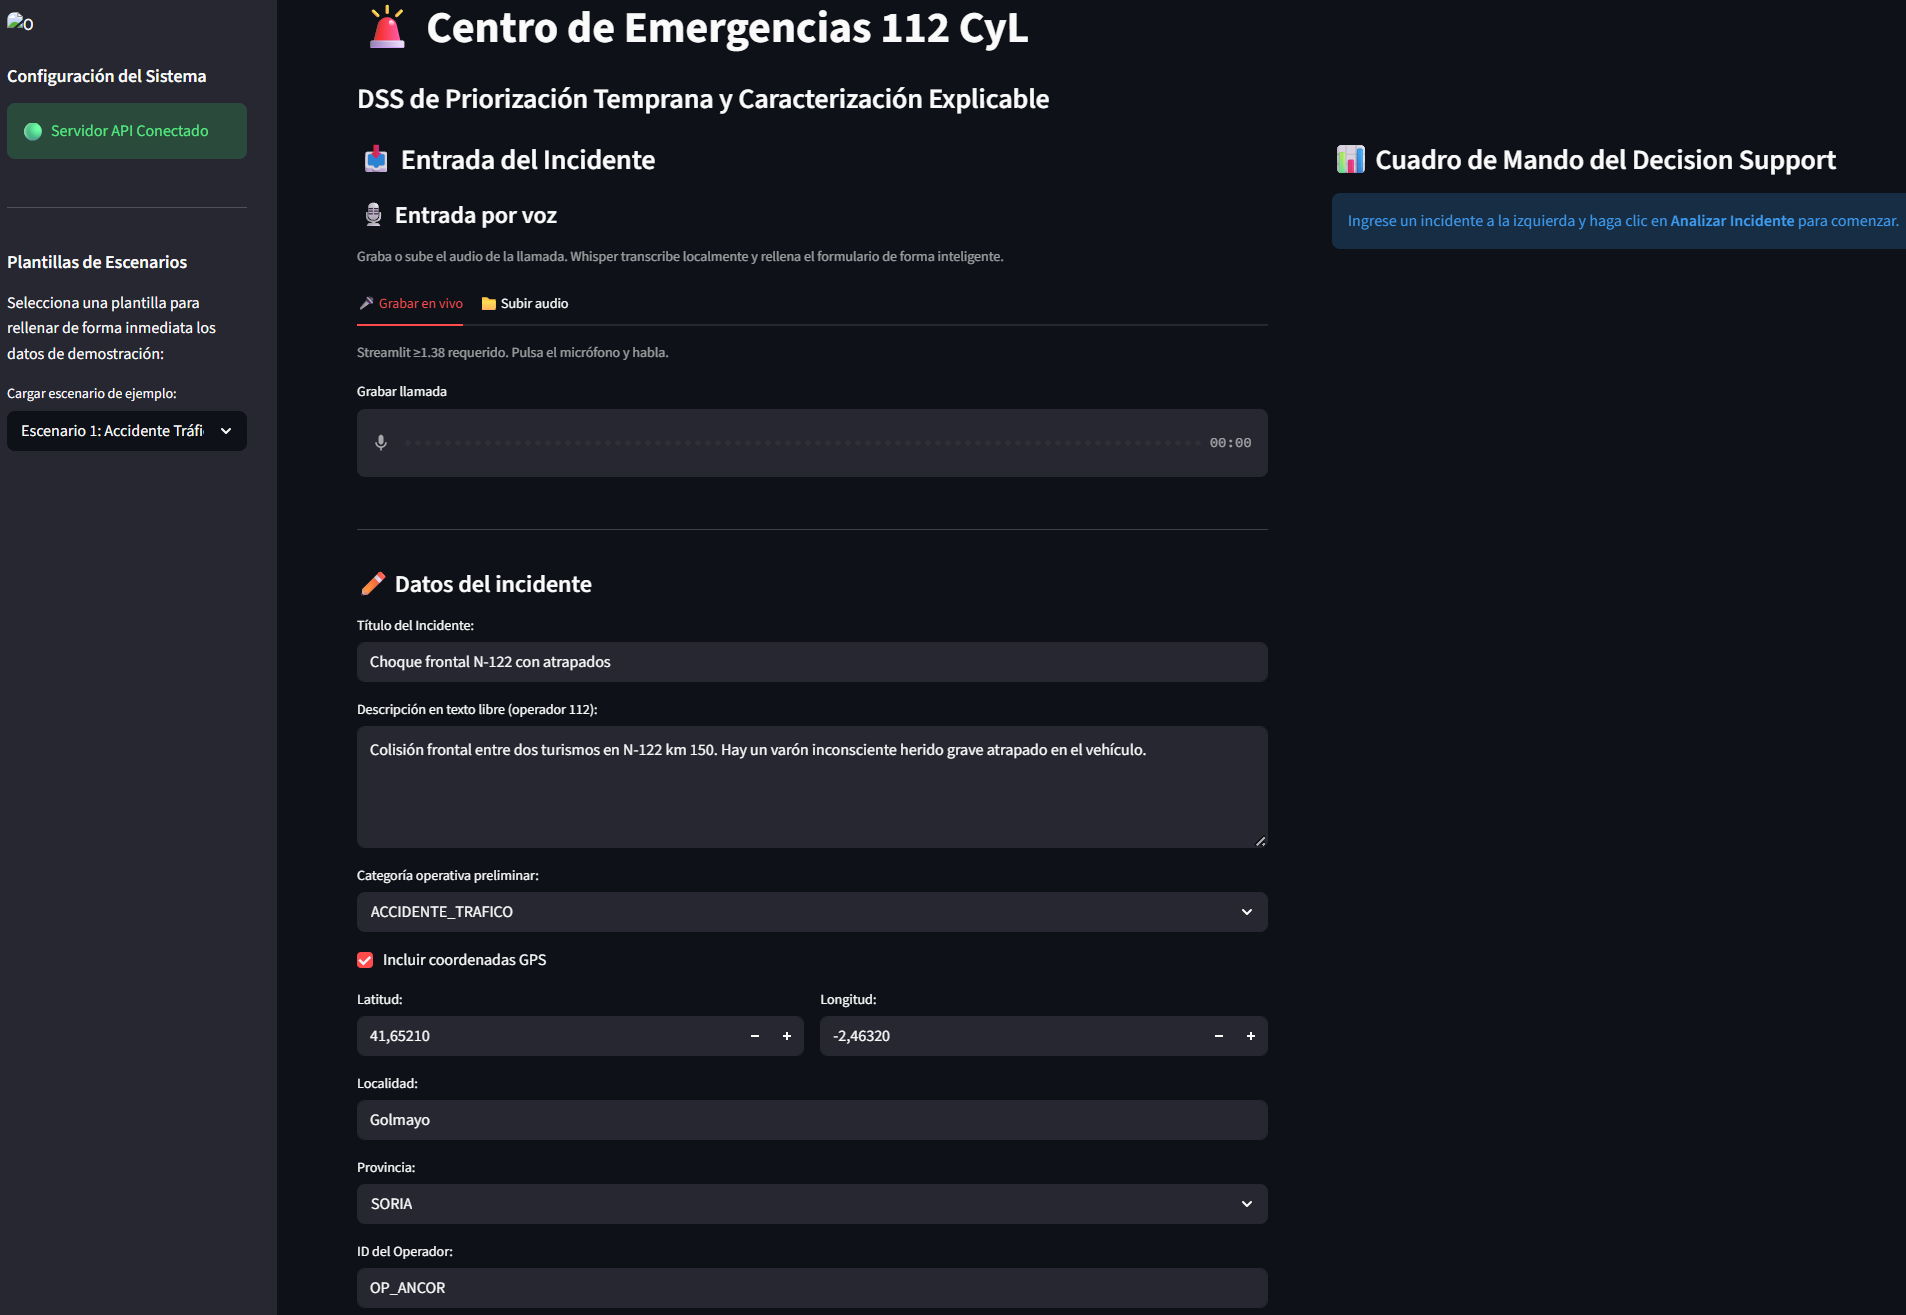
\includegraphics[width=0.88\textwidth]{figures/prototype_v0_1_0/g01_entrada_incidente.png}
    \caption{Entrada manual de un incidente sintético en la interfaz del prototipo.}
    \label{fig:g-entrada}
\end{figure}

\section*{G.3. Entrada de voz experimental}

El módulo de reconocimiento automático del habla (ASR) permite grabar o cargar audio de
prueba y proponer una transcripción para completar el formulario. La persona usuaria
debe revisar y corregir el resultado antes de solicitar una recomendación. Esta
funcionalidad es experimental y no ha sido validada con llamadas reales, ruido de sala
ni locutores representativos.

\begin{figure}[htbp]
    \centering
    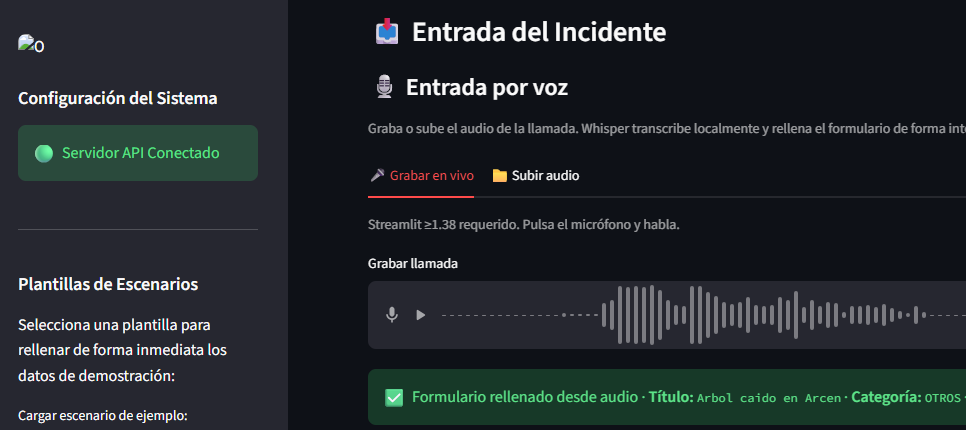
\includegraphics[width=0.82\textwidth]{figures/prototype_v0_1_0/g02_entrada_voz.png}
    \caption{Módulo experimental de entrada por voz mediante \texttt{faster-whisper}.}
    \label{fig:g-voz}
\end{figure}

\section*{G.4. Recomendación interpretable}

La Figura~\ref{fig:g-p1} recoge las dos partes de la salida para un escenario P1. La
interfaz separa la recomendación y distribución de probabilidades de Capa 2 de la
explicación generada por Capa 3. El modelo de lenguaje no modifica la prioridad.

\begin{figure}[htbp]
    \centering
    \begin{minipage}[t]{0.49\textwidth}
        \centering
        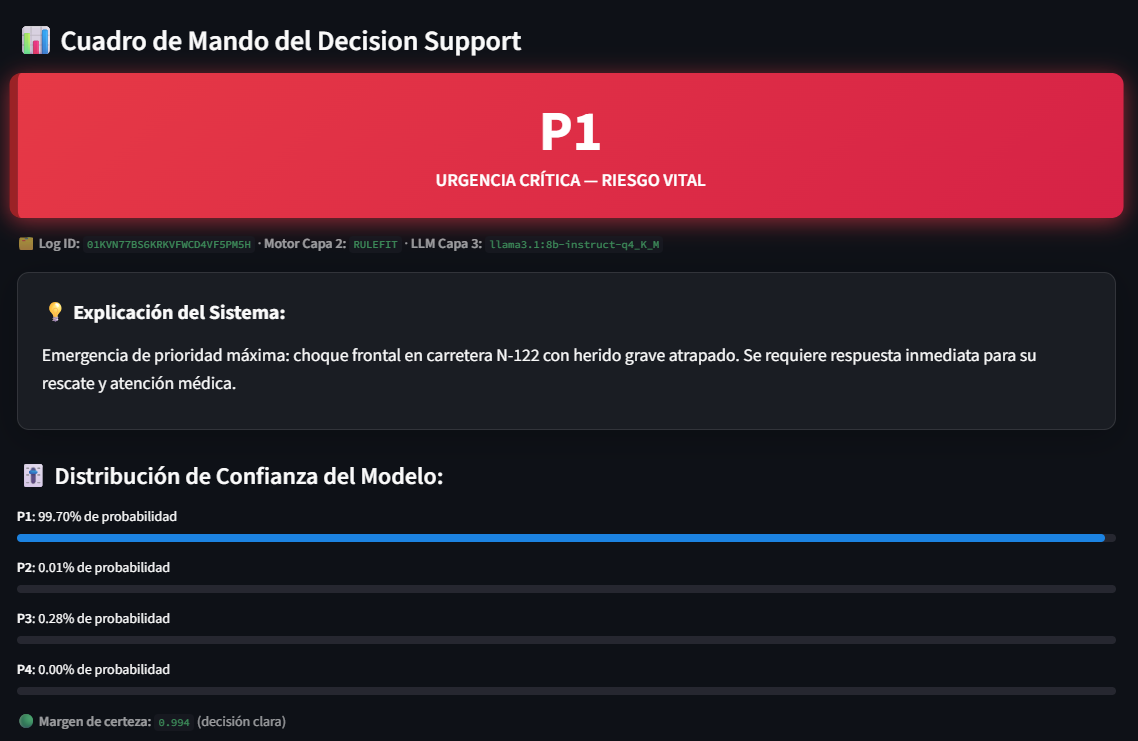
\includegraphics[width=\linewidth]{figures/prototype_v0_1_0/g03_resultado_p1_a.png}
        \small (a) Prioridad y probabilidades.
    \end{minipage}
    \hfill
    \begin{minipage}[t]{0.49\textwidth}
        \centering
        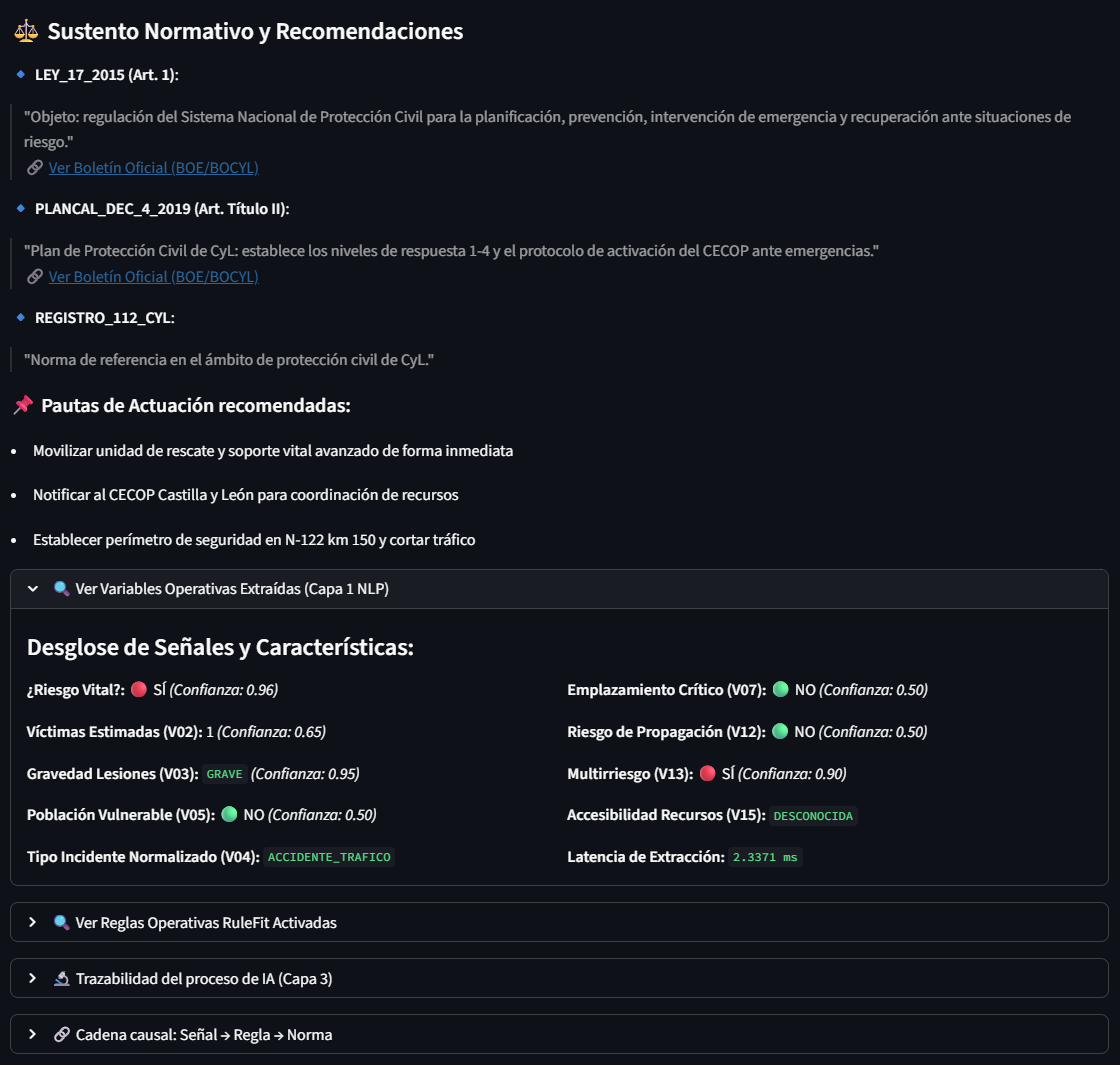
\includegraphics[width=\linewidth]{figures/prototype_v0_1_0/g03_resultado_p1_b.png}
        \small (b) Reglas, explicación y contexto.
    \end{minipage}
    \caption{Resultado de un incidente sintético clasificado como P1.}
    \label{fig:g-p1}
\end{figure}

\section*{G.5. Registro de la decisión humana}

La última evidencia muestra el formulario de retroalimentación. Su finalidad es
registrar si la recomendación se acepta, modifica o rechaza y conservar la justificación
correspondiente. La muestra de 119 casos fue revisada cualitativamente y de forma conjunta
por los tres autores; el formulario queda disponible para una futura evaluación
independiente y trazable, sin que la revisión interna equivalga a validación externa.

\begin{figure}[htbp]
    \centering
    
\includegraphics[width=0.72\textwidth]{figures/prototype_v0_1_0/g06_feedback_humano.png}
    \caption{Formulario para registrar la decisión humana y una posible discrepancia.}
    \label{fig:g-feedback}
\end{figure}

\chapter{Declaración de uso de inteligencia artificial generativa}
\label{cap:anexoh}

\section*{H.1. Declaración}

Durante el desarrollo del TFM se utilizaron asistentes de inteligencia artificial
generativa como herramientas auxiliares de programación, consulta y revisión textual.
Su uso se realizó bajo supervisión de los autores y no sustituyó las decisiones
metodológicas, la ejecución de experimentos, la comprobación de resultados ni la
responsabilidad sobre la versión final de la memoria.

\section*{H.2. Herramientas, finalidad y control}

\begin{table}[htbp]
\centering
\caption{Uso declarado de herramientas de IA generativa}
\label{tab:anexoh-herramientas}
\small
\begin{tabularx}{\textwidth}{|p{3.1cm}|X|p{4.0cm}|}
\hline
\textbf{Herramienta} & \textbf{Uso auxiliar} & \textbf{Control aplicado} \\ \hline
GitHub Copilot \cite{GitHubCopilot2023} & Completado de código, apoyo en depuración y revisión de comentarios técnicos. & Revisión manual, ejecución de pruebas y aceptación expresa de cada cambio. \\ \hline
Asistentes basados en LLM, incluido Google Gemini \cite{GoogleGemini2026} & Consulta técnica, contraste de alternativas, corrección lingüística y apoyo en LaTeX. & Verificación contra código, resultados experimentales y fuentes primarias. \\ \hline
Herramientas de búsqueda asistida & Localización inicial de bibliografía y normativa oficial. & Validación posterior de autoría, fecha, DOI y procedencia oficial. \\ \hline
\end{tabularx}
\end{table}

El equipo utilizó además un enfoque de desarrollo guiado por especificaciones para
coordinar tareas y conservar trazabilidad. Esta organización no genera resultados
académicos por sí misma: las métricas incluidas en la memoria proceden de ejecuciones
reproducibles y fueron revisadas por los autores.

\section*{H.3. Límites y responsabilidad}

Las herramientas generativas no asignaron las etiquetas P1--P4 finales, no eligieron el
modelo de Capa 2 y no determinaron las conclusiones del estudio. La auditoría del
conjunto de datos, el diseño de supervisión débil, el entrenamiento, la evaluación y el
análisis de errores fueron ejecutados mediante procedimientos controlados por el equipo.

Los autores asumen la responsabilidad sobre el código, la selección de fuentes, los
resultados numéricos y la redacción final. El historial del repositorio conserva la
trazabilidad del desarrollo:

\begin{center}
\url{https://github.com/jalbfil/tfe_muia_unir_188}
\end{center}

% Se omite deliberadamente anexo_i.tex para evitar ambiguedad visual entre la letra I
% y el numero romano I. La documentacion de contratos prevista inicialmente se consolida
% en el Anexo F.
\chapter{Corpus normativo para RAG (Capa 3)}
\label{cap:anexoj}

Este anexo presenta de manera detallada el catálogo de leyes, reglamentos y planes de protección civil incorporados al sistema de recuperación de información. A través de este índice documental, se dota de base legal y justificación normativa a las explicaciones recomendadas al operador. Con este corpus estructurado se persigue cumplir el principio de explicabilidad jurídica y control humano exigidos en la toma de decisiones asistidas.

\section*{J.1. Objetivo y alcance}

Este anexo documenta el corpus normativo usado por la Capa 3 en la versión \texttt{v0.1.0}. Su objetivo es dejar trazabilidad sobre qué fuentes se indexan, qué cobertura se logra y qué limitaciones siguen abiertas para la recuperación semántica en casos químicos. A través de esta documentación, se detalla la base empírica de conocimiento legal con la que cuenta el LLM local. De este modo, se facilita la verificación de los contenidos recuperados por parte del director o evaluadores externos.

El corpus se construye en \texttt{resources/corpus\_normativo/} y se indexa en \texttt{artifacts/rag/chroma/} mediante \texttt{scripts/build\_rag\_index.py}. Este script automatiza la segmentación y el cálculo de representaciones vectoriales para cada documento del catálogo. Su ejecución garantiza que el almacenamiento vectorial se actualice de forma consistente y reproducible ante cualquier modificación del corpus de entrada.

\section*{J.2. Método de ingesta e indexación}

La ingesta aplica un pipeline reproducible:

\begin{enumerate}
    \item Lectura de fuentes PDF/HTML oficiales disponibles.
    \item Segmentación en fragmentos (\textit{chunking}) de tamaño aproximado de 400 tokens,
    con solape de 50 tokens.
    \item Enriquecimiento de metadatos por fragmento:
    \texttt{norma\_id}, \texttt{articulo}, \texttt{anio}, \texttt{jerarquia}.
    \item Embeddings con modelo
    \texttt{paraphrase-multilingual-MiniLM-L12-v2}.
    \item Persistencia del índice en ChromaDB local.
\end{enumerate}

La implementación principal del proceso de carga se encuentra en el archivo \texttt{src/capa3\_llm\_mcp/rag/ingestion.py}. Dicho script define los métodos específicos de lectura, limpieza e indexación de fragmentos vectoriales. Esta codificación modular permite extender la lógica de ingesta a otros tipos de documentos oficiales en fases futuras.

\subsection*{J.2.1. Mitigación de vacíos documentales}

Ante la imposibilidad de acceder al texto completo oficial indexable del plan MPCyL
para la versión v0.1.0, se implementó una estrategia de mitigación en la ingesta del
RAG. En el script \texttt{ingestion.py}, durante el procesamiento del PLANCAL, se
inyecta de forma sintética y controlada un fragmento estructurado que describe el
protocolo de actuación ante accidentes de camiones cisterna, fugas químicas y
mercancías peligrosas. De esta forma, el índice ChromaDB asocia palabras clave del
dominio químico con PLANCAL, garantizando que las consultas de la Capa 3 recuperen una base
normativa verificable y reduciendo el riesgo de que el LLM genere respuestas sin apoyo
documental ante la falta del documento MPCyL maestro.

Esta inyección sintética no sustituye al corpus original de MPCyL. Debe interpretarse como una técnica temporal de prototipado para v0.1.0 y resolverse en v0.2.0 mediante la incorporación del texto técnico completo del plan. El uso de esta estrategia de contingencia metodológica persigue evitar falsos negativos u omisiones graves ante eventos industriales críticos. Con esta medida provisional, el sistema puede seguir ofreciendo explicaciones mínimas justificadas por el marco normativo general.

\section*{J.3. Cobertura actual del corpus (v0.1.0)}

Resultado de \texttt{python scripts/build\_rag\_index.py --dry-run}:

\begin{itemize}
    \item LEY\_17\_2015: 64 chunks
    \item RD\_524\_2023: 26 chunks
    \item PLEGEM: 53 chunks
    \item LEY\_4\_2007\_CYL: 67 chunks
    \item PLANCAL\_DEC\_4\_2019: 52 chunks
    \item INFOCAL\_DEC\_6\_2025: 160 chunks
    \item INUNCYL: 3 chunks
    \item LEY\_11\_2022: 330 chunks
    \item RGPD: 202 chunks
    \item LOPDGDD: 151 chunks
    \item REG\_UE\_2024\_1689: 362 chunks
\end{itemize}

Total: \textbf{1470 chunks}.

\section*{J.4. Validaciones de retrieval}

\begin{itemize}
    \item \textbf{T063 (cerrada)}: consulta \textit{atrapado herido grave} con
    recuperación top-1 coherente con Ley 17/2015 art. 1, en consonancia con las directrices de fiabilidad de recuperación RAG en entornos de alta criticidad propuestas por \citeA{Sandeboina2026RAGReliability}.
    \item \textbf{T064 (cerrada en v0.1.0)}: consulta
    \textit{fuga química camión cisterna} con top-1 en conjunto fallback químico
    verificable (PLANCAL/INFOCAL/Ley 17/2015).
\end{itemize}

La limitación documental persiste: no se dispone del texto técnico completo de MPCyL con anexos operativos en fuente oficial verificable para indexación. Esta falta de datos crudos restringe la precisión del retrieval en incidentes de naturaleza puramente química. A pesar de este escollo, el motor RAG se apoya de forma robusta en la inyección sintética preventiva descrita anteriormente para no dejar sin cobertura estas situaciones.

\section*{J.5. Limitación abierta y condición de cierre}

El criterio de cierre de retrieval químico en v0.1.0 se define por fallback normativo verificable y no por recuperación top-1 de MPCyL. Esta decisión pragmática permite cerrar la entrega v0.1.0 con un funcionamiento mínimo defendible. Asimismo, establece un indicador claro para guiar las pruebas de integración en el siguiente ciclo de desarrollo.

Condición de mejora futura (v0.2.0):

\begin{enumerate}
    \item localizar fuente oficial completa de MPCyL;
    \item reingestar y reindexar corpus;
    \item repetir prueba de retrieval químico con evidencia de top-1 MPCyL.
\end{enumerate}

\section*{J.6. Trazabilidad de artefactos}

Artefactos relacionados con este anexo:

\begin{itemize}
    \item \texttt{artifacts/rag/chroma/}
    \item \texttt{tests/test\_rag\_retrieval.py}
    \item \texttt{specs/001-priorización-112-cyl/tasks.md} (T060--T065)
\end{itemize}

\chapter{Prompts y herramientas MCP de Capa 3}
\label{cap:anexok}

Este anexo detalla los mecanismos de interacción entre el modelo generativo local y el resto de componentes a través del protocolo MCP. En particular, se describen las plantillas de instrucciones y los parámetros configurados para asegurar explicaciones fieles a la decisión predictiva. Con esta documentación técnica se persigue dar transparencia al proceso de generación lingüística y mitigar posibles riesgos de desalineación.

\section*{K.1. Objetivo}

Este anexo describe cómo la Capa 3 transforma la salida congelada de la Capa 2 en una explicación estructurada para la supervisión humana. El principio operativo es invariable: \textbf{la prioridad P1--P4 la decide la Capa 2}; la Capa 3 solo explica, cita y contextualiza. A través de este aislamiento, se asegura que el comportamiento probabilístico del LLM no interfiera con el clasificador estadístico. De este modo, se evitan cambios arbitrarios en el nivel de emergencia asignado.

\section*{K.2. Entradas y salida esperada}

La Capa 3 consume principalmente dos bloques del endpoint
\texttt{/predict}:

\begin{itemize}
    \item \texttt{priority\_details}: prioridad, distribución de probabilidades,
    confianza, modelo usado y reglas activadas.
    \item \texttt{explanation\_context}: decisión de la Capa 2,
    \texttt{probability\_margin}, resumen de reglas, evidencias y avisos.
\end{itemize}

Salida contractual de la Capa 3: \texttt{OperatorRecommendation} con \texttt{priority\_recommended}, \texttt{explanation\_text}, \texttt{legal\_citations}, \texttt{actuation\_hints} y metadatos del LLM. Esta estructura de datos se encuentra totalmente definida y validada mediante esquemas JSON robustos. Con ella se asegura la consistencia e integridad de las respuestas que se muestran en el panel del despachador.

\begin{table}[ht]
\centering
\caption{Campos principales del JSON explicativo de la Capa 3}
\label{tab:anexok-json}
\small
\begin{tabularx}{\textwidth}{|p{3.5cm}|X|}
\hline
\textbf{Campo} & \textbf{Directriz operativa} \\ \hline
\texttt{explanation\_text} & Explicación breve, formal y accionable, entre 80 y 600 caracteres, sin recalcular prioridad ni introducir hechos nuevos. \\ \hline
\texttt{actuation\_hints} & Lista de acciones orientativas coherentes con P1--P4, siempre sometidas al criterio del operador. \\ \hline
\texttt{confidence\_disclaimer} & Advertencia sobre falta de información, baja confianza o discrepancias entre la prioridad calculada y el texto original. \\ \hline
\end{tabularx}
\end{table}

\section*{K.3. Política de prompts (v0.1.0)}

Los prompts de sistema y ejemplos \textit{few-shot} están orientados a:

\begin{enumerate}
    \item mantener la prioridad calculada por la Capa 2;
    \item explicar incertidumbre cuando el margen de probabilidad es bajo;
    \item justificar la recomendación con reglas/evidencias reales;
    \item incluir cita legal mínima en casos P1/P2.
\end{enumerate}

Reglas de seguridad del prompt:

\begin{itemize}
    \item no recalcular prioridad;
    \item no inventar reglas ni citas cuando no hay evidencia;
    \item declarar necesidad de revisión humana ante baja confianza.
\end{itemize}

Archivos de referencia: \texttt{src/capa3\_llm\_mcp/prompts/system\_prompt.py} y \texttt{src/capa3\_llm\_mcp/prompts/few\_shots.py}. En estos módulos de código fuente se definen las instrucciones de comportamiento del modelo de lenguaje y las muestras guías. Su edición directa permite ajustar el estilo de las explicaciones generadas sin alterar el motor predictivo principal.

\section*{K.3.1. Directrices éticas y de seguridad en prompts}

Los prompts de la Capa 3 incorporan instrucciones específicas para evitar rechazos
genéricos propios de asistentes comerciales. Dado que un LLM instruido puede negarse a
procesar textos sobre violencia, accidentes, sustancias químicas o situaciones de
peligro, el \texttt{SYSTEM\_PROMPT} redefine su rol como soporte exclusivo de seguridad
pública. Se le prohíbe denegar el procesamiento de descripciones críticas y se le exige
emitir un JSON completo y supervisable.

Asimismo, el prompt define una directriz de detección de discrepancias: si el modelo
identifica incoherencias entre la prioridad precalculada por la Capa 2 y los hechos
descritos en el texto, por ejemplo una prioridad P3/P4 ante riesgo vital, inconsciencia,
atrapados o materiales peligrosos, debe alertar en el campo
\texttt{confidence\_disclaimer}. Esta alerta no modifica la prioridad, pero incentiva la
revisión humana.

\section*{K.4. Herramientas MCP activas en v0.1.0}

En \texttt{v0.1.0} se registran tres tools:

\begin{itemize}
    \item \texttt{search\_normative}
    \item \texttt{get\_rule\_details}
    \item \texttt{cite\_legal\_basis}
\end{itemize}

Implementación del servidor MCP y sus herramientas asociadas en: \texttt{src/capa3\_llm\_mcp/mcp\_server/server.py} y \texttt{src/capa3\_llm\_mcp/mcp\_server/tools/}. Dicho código define el catálogo de funciones que el modelo puede invocar para enriquecer su respuesta. Esta arquitectura abierta simplifica el mantenimiento y la integración de nuevos recursos del sistema.

La tool \texttt{get\_aemet\_context} queda diferida a \texttt{v0.2.0} según alcance aprobado. Su implementación en el servidor de herramientas requiere la provisión de una API de meteorología robusta. No obstante, para el alcance del actual prototipo, se ha preservado la definición formal en la especificación para mantener la compatibilidad futura.

\section*{K.5. Runtime LLM y modo degradado}

El runtime operativo en \texttt{v0.1.0} usa Ollama local con el modelo por defecto \texttt{llama3.1:8b-instruct-q4\_K\_M}, configurable por variable \texttt{OLLAMA\_MODEL}. El wrapper mantiene el nombre histórico \texttt{QwenWrapper} por compatibilidad de código. Esta modularidad del backend facilita cambiar el motor de inferencia local sin reescribir la lógica de negocio. Con ello se asegura que el sistema pueda adaptarse a modelos más eficientes que se publiquen en el futuro.

Si el LLM no está disponible o la respuesta no cumple con el contrato, se activa el modo
degradado determinista:

\begin{itemize}
    \item se conserva la prioridad de la Capa 2;
    \item se construye una explicación basada en reglas y probabilidades;
    \item se preserva la exigencia de citas mínimas para P1/P2.
\end{itemize}

El orquestador implementa además una recuperación robusta del JSON mediante extracción
del primer objeto válido devuelto por el modelo. Si la respuesta queda corrupta o no
puede validarse contra \texttt{OperatorRecommendation}, el sistema cae de forma segura en
modo degradado basado en reglas, evitando que un fallo de formato bloquee la salida.

\section*{K.6. Límites conocidos}

\begin{itemize}
    \item la latencia con LLM real depende del hardware local y de la carga del
    runtime Ollama;
    \item el soporte normativo para escenarios químicos sigue condicionado por la
    cobertura documental de MPCyL (ver Anexo~\ref{cap:anexoj});
    \item la evaluación con un juez LLM independiente queda como ampliación futura
    respecto al juez determinista offline ya aplicado en la versión v0.1.0.
\end{itemize}

\chapter{Fichas de las capas}
\label{cap:anexol}

\section*{L.1. Alcance}

Este anexo resume la finalidad, entradas, salidas, evaluación y limitaciones de las
tres capas. La separación de responsabilidades es esencial: Capa 1 estructura el texto,
Capa 2 recomienda la prioridad y Capa 3 explica esa recomendación. La persona operadora
mantiene la decisión final.

Los detalles anteriormente distribuidos entre los anexos técnicos de recuperación
normativa y configuración del LLM se consolidan aquí para ofrecer una visión académica
única y evitar inventarios de rutas, clases o ficheros.

\section*{L.2. Capa 1: extracción NLP simbólica}

\textbf{Finalidad.} Transformar el título y la descripción del incidente en variables
predecisionales estructuradas. El procedimiento combina detección semántica mediante
reglas y diccionarios operativos, tratamiento de negaciones, normalización de valores y
estimación de confianza. La salida conserva la señal activada y su procedencia para
facilitar la auditoría.

\textbf{Evaluación.} Sobre cinco escenarios curados obtiene precisión micro
(0{,}733333), sensibilidad micro (1{,}000000), F1 micro (0{,}846154) y latencia
media (4{,}58844) ms. Es una comprobación funcional reducida, no una validación sobre
llamadas reales ni sobre un conjunto de referencia etiquetado por el 112.

\textbf{Limitación.} La versión evaluada no contiene un clasificador aprendido
congelado ni se le atribuyen entrenamientos o métricas procedentes de la Capa 2. La
posible incorporación de modelos aprendidos queda como trabajo futuro y requeriría una
evaluación específica.

\section*{L.3. Capa 2: priorización interpretable}

\subsection*{L.3.1. Datos y etiqueta objetivo}

La Capa 2 se entrena y evalúa con 9.380 registros limpios del Registro 112 Castilla y
León. La prioridad P1--P4 no existe en la fuente: es una etiqueta académica construida
mediante supervisión débil. El acuerdo principal alcanza un alfa de Krippendorff de
\(\alpha = 0{,}899902\). Las particiones utilizadas exclusivamente para Capa 2 son 6.512
registros de entrenamiento, 1.415 de validación y 1.453 de prueba; la prueba temporal de
2022 contiene 735 registros.

Las variables de entrada se limitan a señales disponibles antes de la primera decisión:
fallecimiento, herido grave, atrapamiento, intoxicación, llamadas múltiples, incendio,
accidente de tráfico, rescate, meteorología o inundación, riesgo vital textual y
categoría preliminar normalizada. Se excluyen recursos movilizados, pacientes atendidos,
cierre del incidente y cualquier información posterior, con el fin de evitar fugas de
información.

\subsection*{L.3.2. Alternativas y selección}

Se comparan una línea base de 19 reglas expertas, RuleFit-lite y una implementación
externa de RuleFit mediante \texttt{imodels} \cite{Singh2021imodels}. Esta última se
utiliza con finalidad diagnóstica. La selección se realiza con la partición de validación
y la estimación final se obtiene una sola vez sobre la partición de prueba.

\begin{table}[htbp]
\centering
\caption{Resultados de los modelos de Capa 2 en la partición de prueba}
\label{tab:model-card-capa2-comparativa}
\small
\begin{tabular}{|l|r|r|r|r|}
\hline
\textbf{Modelo} & \textbf{Exactitud} & \textbf{Macro-F1} & \textbf{Sensibilidad P1} & \textbf{Reglas} \\ \hline
Línea base heurística & 0,694425 & 0,464284 & 0,998473 & 19 \\ \hline
RuleFit-lite & 0,903648 & 0,905604 & 0,909924 & 30 \\ \hline
RuleFit externo & 0,768385 & 0,568239 & 0,902778 & 30 \\ \hline
\end{tabular}
\end{table}

RuleFit-lite se selecciona porque presenta la mejor macro-F1, mantiene una sensibilidad
P1 superior al umbral interno de (0{,}85), conserva reglas exportables y ofrece menor
coste local que la configuración externa ensayada. En la prueba temporal alcanza
exactitud (0{,}884354), macro-F1 (0{,}877594) y sensibilidad P1 (0{,}928767).

Estas métricas corresponden al estimador RuleFit-lite \textbf{sin Puerta de Seguridad}.
La salvaguarda es una función determinista de posprocesamiento aplicada durante la
inferencia integrada; se comprueba mediante escenarios funcionales y no se mezcla con
la comparación estadística de modelos.

\subsection*{L.3.3. Riesgos y trazabilidad}

La matriz de confusión identifica 59 falsos negativos P1: 34 casos clasificados como
P2, 18 como P3 y 7 como P4. Los siete errores P1--P4 constituyen el riesgo principal y
forman parte de la muestra de 119 casos preparada para revisión. Los campos reservados
a la persona revisora permanecen vacíos, por lo que esta muestra no equivale a una
validación humana completada.

\section*{L.4. Capa 3: explicación local y recuperación normativa}

\textbf{Finalidad.} Capa 3 recibe la prioridad, las probabilidades, las reglas activadas
y el contexto explicativo generado por Capa 2. Produce una explicación estructurada y
evidencias normativas, pero no recalcula ni modifica la prioridad.

\textbf{Recuperación.} El sistema utiliza un índice semántico local sobre normativa
estatal y de Castilla y León. Los documentos se segmentan y representan con el modelo
multilingüe \texttt{paraphrase-multilingual-MiniLM-L12-v2}. La cobertura incluye la
legislación de protección civil y los planes territoriales y especiales disponibles. No
se dispone del texto técnico completo de MPCyL, por lo que la recuperación en escenarios
químicos debe interpretarse con cautela y completarse en una versión futura con la
fuente oficial íntegra.

\textbf{Generación y salvaguardas.} El LLM se ejecuta localmente con temperatura
(0{,}0). Las instrucciones exigen mantener la prioridad de Capa 2, utilizar solo las
reglas y evidencias recibidas, declarar incertidumbre y evitar hechos o citas no
recuperados. Las herramientas de consulta normativa y detalle de reglas se exponen de
forma controlada mediante Model Context Protocol. Si el modelo no responde o incumple
el contrato, se genera una explicación alternativa determinista que conserva la salida
de Capa 2.

\textbf{Evaluación.} La prueba funcional con LLM local resuelve correctamente cuatro
escenarios P1--P4 y observa una latencia media de (4{,}898) s en el entorno
experimental. La evaluación automatizada de fidelidad sobre los 119 casos preparados
alcanza una tasa de cumplimiento de (1{,}000000), fidelidad media (0{,}957367) y
mínima (0{,}933333). Se trata de un juez determinista sobre explicaciones controladas,
no de una evaluación humana ni de un LLM-as-Judge independiente.

\section*{L.5. Entrada de voz experimental}

La interfaz incorpora reconocimiento automático del habla mediante
\texttt{faster-whisper}. Su salida propone texto y campos normalizados que deben
revisarse antes de ejecutar la inferencia. Esta función se ha utilizado como demostración
con audio de prueba; no se reportan tasas de error de palabra ni validación con llamadas
reales, ruido de sala o diversidad de locutores.

\section*{L.6. Limitaciones comunes}

\begin{itemize}
    \item La referencia P1--P4 es académica y débil, no una prioridad oficial del 112.
    \item Las pruebas integradas muestran compatibilidad técnica en escenarios
    controlados, no utilidad operativa ni cumplimiento de un acuerdo de nivel de servicio.
    \item La Puerta de Seguridad es una salvaguarda conservadora no certificada y debe
    evaluarse separadamente del modelo estadístico.
    \item La muestra de 119 casos está preparada para revisión, pero no contiene
    decisiones humanas completadas.
    \item Los resultados no acreditan conformidad regulatoria ni autorizan el uso del
    prototipo en un servicio de emergencias real.
\end{itemize}


\end{document}

